
\documentclass[11pt,a4paper]{article}                           

\usepackage[bookmarksopen, bookmarksnumbered, bookmarksopenlevel=2]{hyperref}
\usepackage{tikz}
\usepackage{tikz-3dplot}
\usetikzlibrary{calc}
\usetikzlibrary{decorations} %
\usepackage{ngerman}
\usepackage[UKenglish]{babel}
\usepackage[toc,page]{appendix}
\usepackage{amsmath}
\usepackage{amssymb}
\usepackage{graphicx}
\usepackage{hhline}
\usepackage[bf]{caption}
\usepackage{cite}
\usepackage[vcentermath]{youngtab}
\usepackage{geometry}
\usepackage{float}
\usepackage{epstopdf}

\usepackage{subfig} % zwei Bilder nebeneinander


\usepackage{wrapfig}	 

\geometry{verbose,a4paper,tmargin=30mm,bmargin=25mm,outer=20mm,inner=20mm,bindingoffset=0mm}
\usepackage{pgfplots}
\pgfplotsset{width=7cm} 

\DeclareSymbolFont{bbold}{U}{bbold}{m}{n}
\DeclareSymbolFontAlphabet{\mathbbold}{bbold}
\newcommand{\one}{\mathbbold{1}}
 



\newcommand{\IF}{\text{Im}\, \mathcal{F}}
\newcommand{\IM}{\text{Im}\, \mathcal{M}}
\newcommand{\RF}{\text{Re}\, \mathcal{F}}
\newcommand{\RM}{\text{Re}\, \mathcal{M}}
\newcommand{\I}{\text{Im}}
\newcommand{\R}{\text{Re}}

\newcommand{\Kcs}{K_{\text{cs}}}
\newcommand{\Kks}{K_{\text{ks}}}

\newcommand{\volume}{\text{{\small} vol}\, }


\newcommand{\un}{{\bf 1}}
\newcommand{\unb}{{\bf \bar{1}}}
\newcommand{\f}{{\bf 5}}
\newcommand{\fb}{{\bf \bar{5}}}
\newcommand{\te}{{\bf 10}}
\newcommand{\teb}{{\bf \bar{10}}}
\newcommand{\op}{\oplus}
\newcommand{\ot}{\otimes}
\newcommand{\ad}{\mathrm{ad}}
\newcommand{\Z}{\mathbb{Z}}

\usepackage{cancel}



%%%%%%%%%%%%%%%%%%%%%%%%%%%%%%%%%%%%%%%%%%%%%%%
%%%%%%%%%%%%%%%%%%%%%%%%%%%%%%%%%%%%%%%%%%%%%%%
%%%%%%%%%%%%%%%%%%%%%%%%%%%%%%%%%%%%%%%%%%%%%%%
%%%%%%%%%%%%%%%%%%%%%%%%%%%%%%%%%%%%%%%%%%%%%%%

%%%%%%%%%%%%%%%%%%%%%%%%%%%%%%%%%%%%%%%%%%%%%%%
\hypersetup{
    pdftitle={},
    pdfauthor={David Gerick},
    pdfsubject={HGSFP Winter School 2017 evaluation}
}
%
\numberwithin{equation}{section}
\numberwithin{table}{section}\setlength{\multlinegap}{25pt}  

%%%%%%%%%%%%%%%%%%%%%%%%%%%%%%%%%%%%%%%%%%%%%%%%%%%%%%%

\newcommand{\bea}{\begin{eqnarray}}
\newcommand{\eea}{\end{eqnarray}}

\newcommand{\tw}{{\rm w}}


\newcommand{\executeiffilenewer}[3]{%
 \ifnum\pdfstrcmp{\pdffilemoddate{#1}}%
 {\pdffilemoddate{#2}}>0%
 {\immediate\write18{#3}}\fi%
}
\newcommand{\includesvg}[1]{%
 \executeiffilenewer{#1.svg}{#1.pdf}%
 {inkscape -z -D --file=#1.svg %
  --export-pdf=#1.pdf --export-latex}%
   \input{#1.pdf_tex}%
}
%%%%%%%%%%%%%%%%%%%%%%%%%%%%%%%%%%%%%%%%%%%%%%%%%%%%%%%



%%%%%%%%%%%%%%%%%%%%%%%%%%%%%%%%%%%%%%%%%%%%%%%
%%%%%%%%%%%%%%%%%%%%%%%%%%%%%%%%%%%%%%%%%%%%%%%
%%%%%%%%%%%%             %%%%%%%%%%%%%%%%%%%%%%
%%%%%%%%%%%%  TITLEPAGE  %%%%%%%%%%%%%%%%%%%%%%
%%%%%%%%%%%%             %%%%%%%%%%%%%%%%%%%%%%
%%%%%%%%%%%%%%%%%%%%%%%%%%%%%%%%%%%%%%%%%%%%%%%
%%%%%%%%%%%%%%%%%%%%%%%%%%%%%%%%%%%%%%%%%%%%%%%
%%%%%%%%%%%%%%%%%%%%%%%%%%%%%%%%%%%%%%%%%%%%%%%

\begin{document}

\baselineskip=14pt
\parskip 5pt plus 1pt 


\vspace*{-1.5cm}
\begin{flushright}    % Publication numbers
  {\small

  }
\end{flushright}

\vspace{2cm}
\begin{center}        % Main title
  {\LARGE 10th HGSFP Winter School}\\
   {\Large Obergurgl 2017}\\
   \vspace{2cm}
   {\LARGE \bf Final Report}
\end{center}
\pagestyle{empty}
\vspace{12cm}
%
\subsection*{Organization Team}
	Heiko Augustin \\
	David Gerick \\
	Lennart Huth \\
	Frank K\"onnig \\
	Janko Nauta \\
	Merve \c{S}ahinsoy \\
%%%%%%%%%%%%%%%%%%%%%%%%%%%%%%%%%%%%%%%%%%%%%%%
%%%%%%%%%%%%%%%%%%%%%%%%%%%%%%%%%%%%%%%%%%%%%%%
%%%%%%%%%%%%%%%%%%%%%%%%%%%%%%%%%%%%%%%%%%%%%%%

%%%%%%%%%%%%%%%%%%%%%%%%%%%%%%%%%%%%%%%%%%%%%%%
%%%%%%%%%%%%%%%%%%%%%%%%%%%%%%%%%%%%%%%%%%%%%%%
%%%%%%%%%%%                 %%%%%%%%%%%%%%%%%%%
%%%%%%%%%%%  DOCUMENT BODY  %%%%%%%%%%%%%%%%%%%
%%%%%%%%%%%                 %%%%%%%%%%%%%%%%%%%
%%%%%%%%%%%%%%%%%%%%%%%%%%%%%%%%%%%%%%%%%%%%%%%
%%%%%%%%%%%%%%%%%%%%%%%%%%%%%%%%%%%%%%%%%%%%%%%
%%%%%%%%%%%%%%%%%%%%%%%%%%%%%%%%%%%%%%%%%%%%%%%

\newpage
\setcounter{page}{1}

\pagestyle{plain}

\section{Report Winter School 2017}

This document concludes the 10th HGSFP Winter School, which took place for the tenth time at the University Center in Obergurgl, Austria from January 27th 2017 to January 31st 2017. In total 49 students - as we had one cancellations at short notice due to illness, we could not fill all 50 places - attended the lectures and participated in the poster sessions and social activities at the center and in the Obergurgl ski area. 

\subsection*{Bus transfer from and to Heidelberg}
TODO: Heiko

\subsection*{The venue}

TODO: Lennart
%The staff at the University Center was, as always, very helpful and as previous years all activities and practical arrangements went smoothly during our stay in Obergurgl.

\subsection*{Scientific program}

TODO: Frank

\noindent The scientific program consisted of three main parts: 
\begin{itemize}
\item The scientific talks, on topics representing all the HGSFP branches and with the aim of introducing the research conducted at the different institutes in an accessible way to non-experts in the area. 
\item The two poster sessions, during which all participants presented their research.
\item The special invitation talk, which by tradition has some relation to the Tirol area and a wider scientific scope than the subject specific talks. 
\end{itemize}

The lecture schedule (see Appendix A), easily available in the provided book of abstracts, encouraged all participants to attend lectures on topics different from their research subjects. The lecturers stayed at the University Center for either the entire school or part of it, thus giving lots of opportunities to discuss their talks and projects with them in a relaxed environment. \\
During the two poster sessions the participants presented their research to each other. Despite the tough schedule the discussions during these evenings were very intense and fruitful. With the lectures as a common basis the posters often served as a source for in-depth discussions of various theoretical and experimental phenomena. \\
The invitation lecture this year focussed on the danger of glaciers and snow production. It covered the glacier's scientific history from first reports of early explorers and field measurements until modern glaciology which by numerical modelling and remote sensing is a valuable tool for climate science. Furthermore, it discussed several aspects of snow production in the alps which is quite important for the local tourist sector.

\subsection*{Social event}

TODO: Janko

The first evening of the Winter School was devoted to a social event - Eisstockschie{\ss}en - which is by now a tradition of this school. The local supervision was very nice and the evening as a whole very appreciated by the participants.\\

A new organising commitee for next year's Winter School was already formed during this Winter School. Although the accommodation facilities were well appreciated by all participants, we have animated the new committee to search for possible cheaper alternatives for the Winter School in 2018 as the expenses for accommodation at the University Center in Obergurgl have steadily increased over the last couple of years.
\\
The results of the evaluation sheets are presented in Appendix B, showing that the school in general and the scientific program in particular was well received by the participating students.\\

\noindent We want to thank the HGSFP for the financial support that made the 2016 Winter School possible.


\newpage
\appendix
\section{Schedule of the HGSFP Winterschool 2016}

\begin{figure}[H]
\centering
%\vspace{-7.6cm}
%\hspace*{-0.7cm}
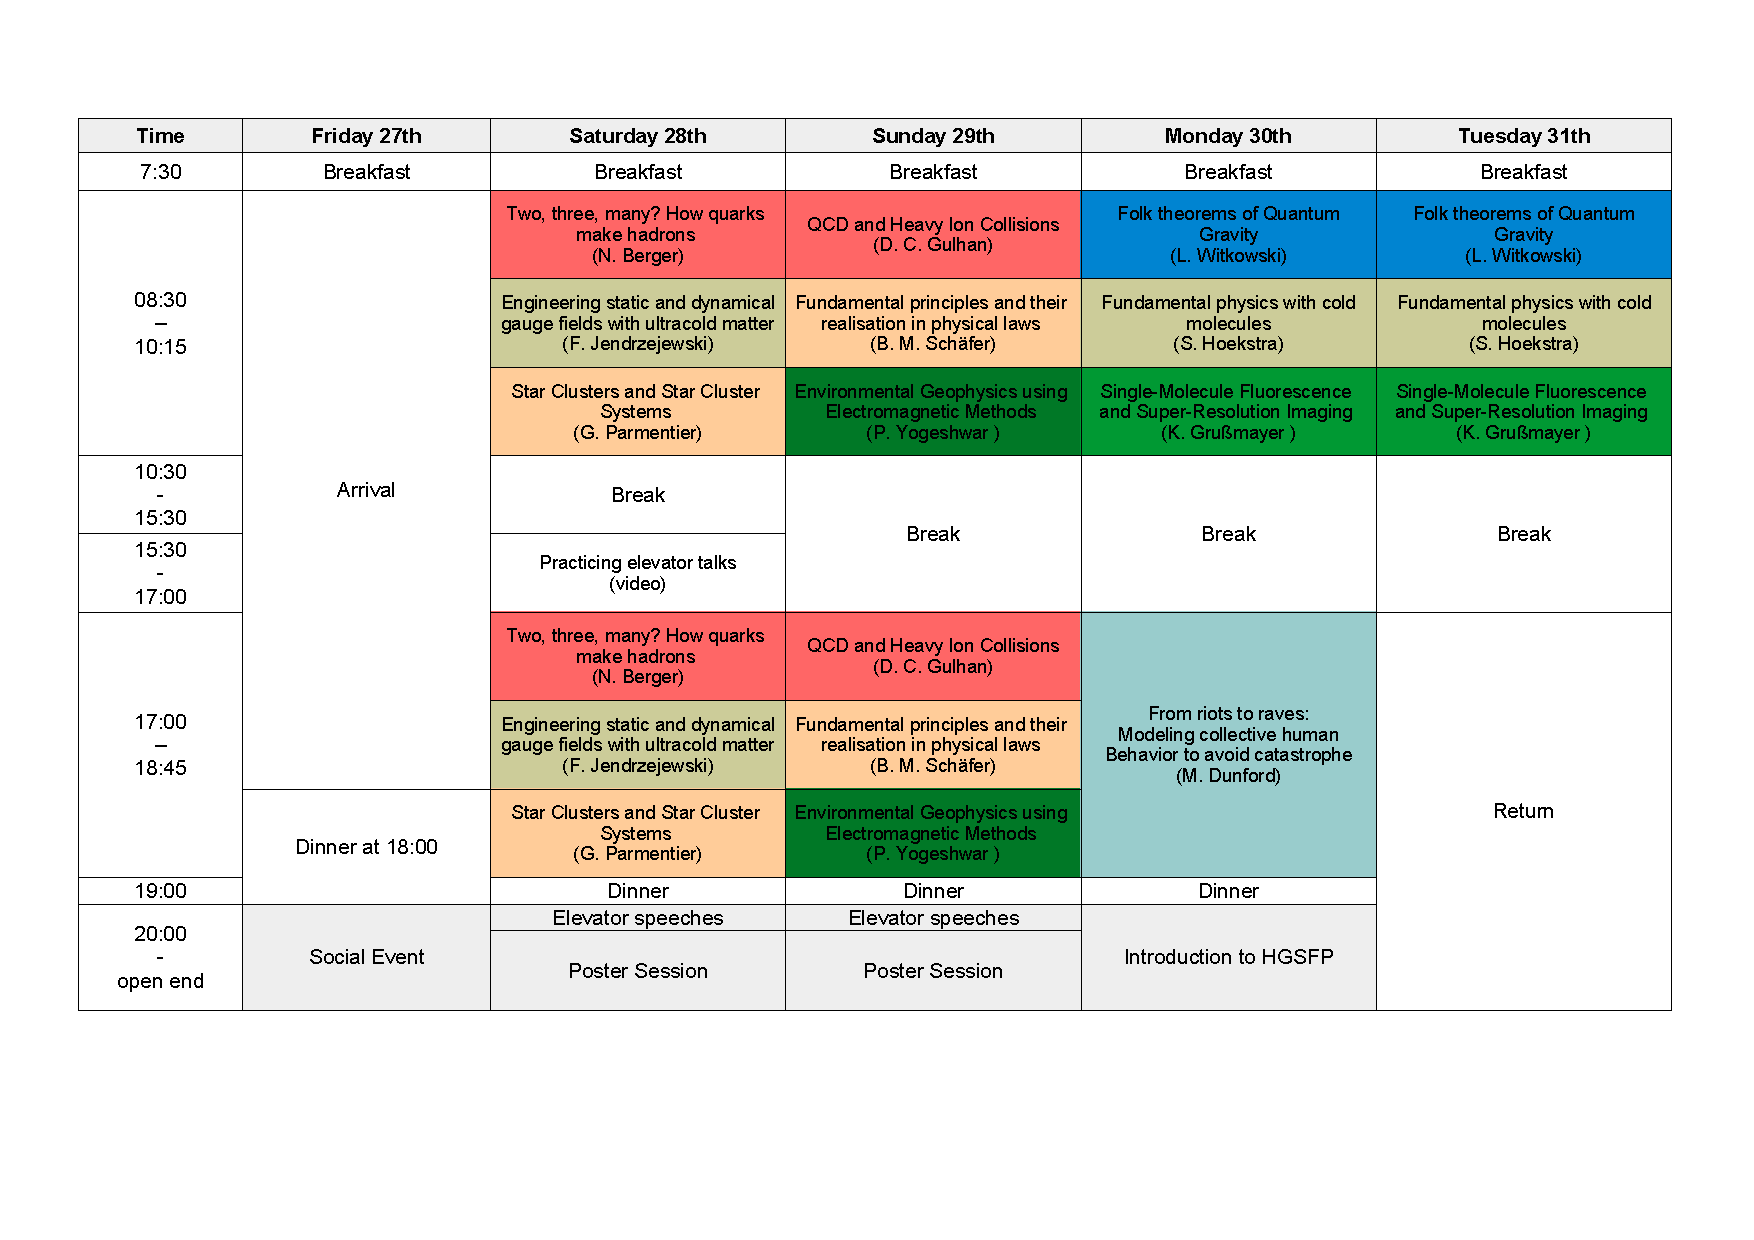
\includegraphics[angle=90,width=0.999\textwidth]{FinalProgram.pdf}
%\vspace{-1.5cm}
\caption{The HGSFP Winter School 2017 schedule.}
\end{figure}
\newpage
\section{General Evaluation}
Below we present the statistics from the evaluation sheets which were distributed in the bus on the way back to Heidelberg. The questions concern the school in general, the scientific talks and includes comments from the participants. The distribution of the answers among the HGSFP branches was as follows: \\ \\

\subsubsection{General}

\begin{figure}[H]
\centering
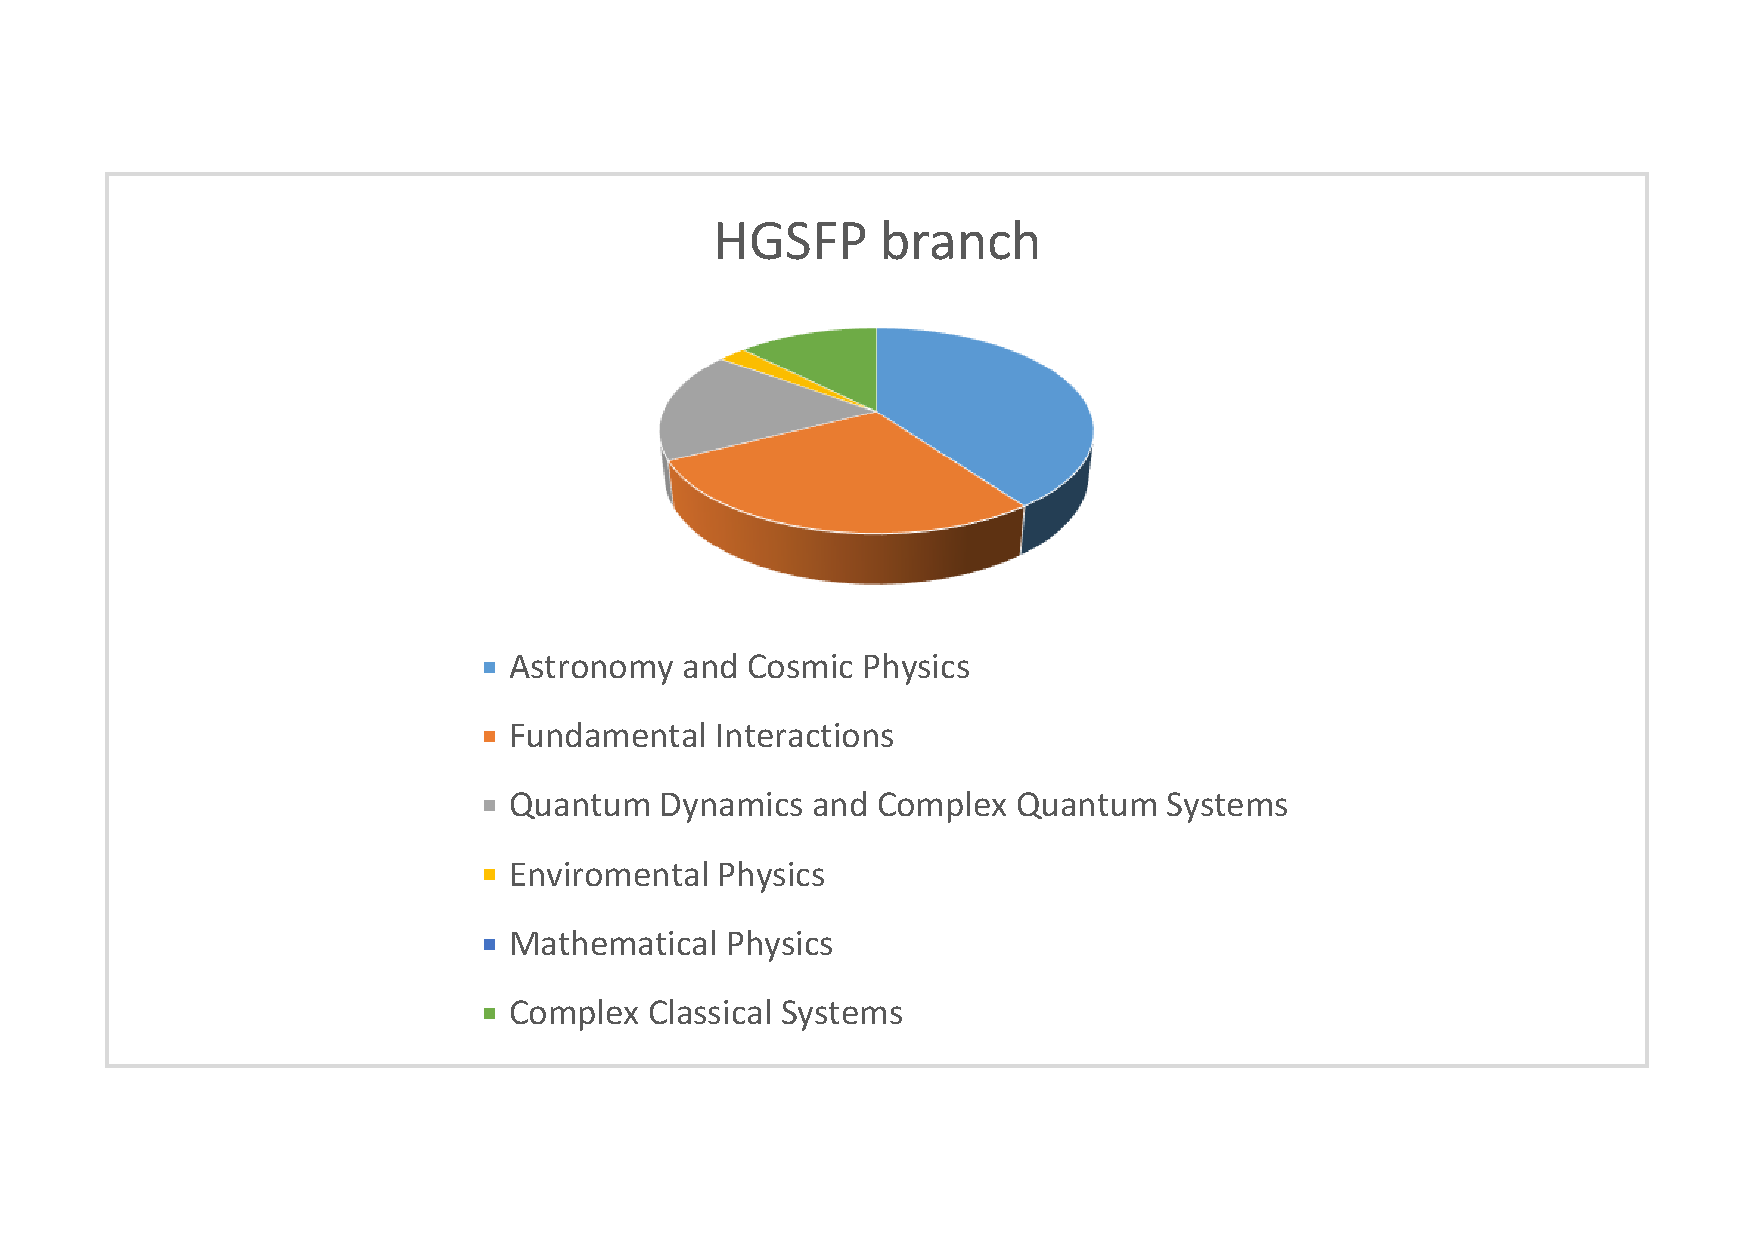
\includegraphics[width=0.8\textwidth]{eval/general/hgsfp_branch.pdf}
\caption{In which branch of the HGSFP are you?}
\end{figure}
\begin{figure}[H]
\centering
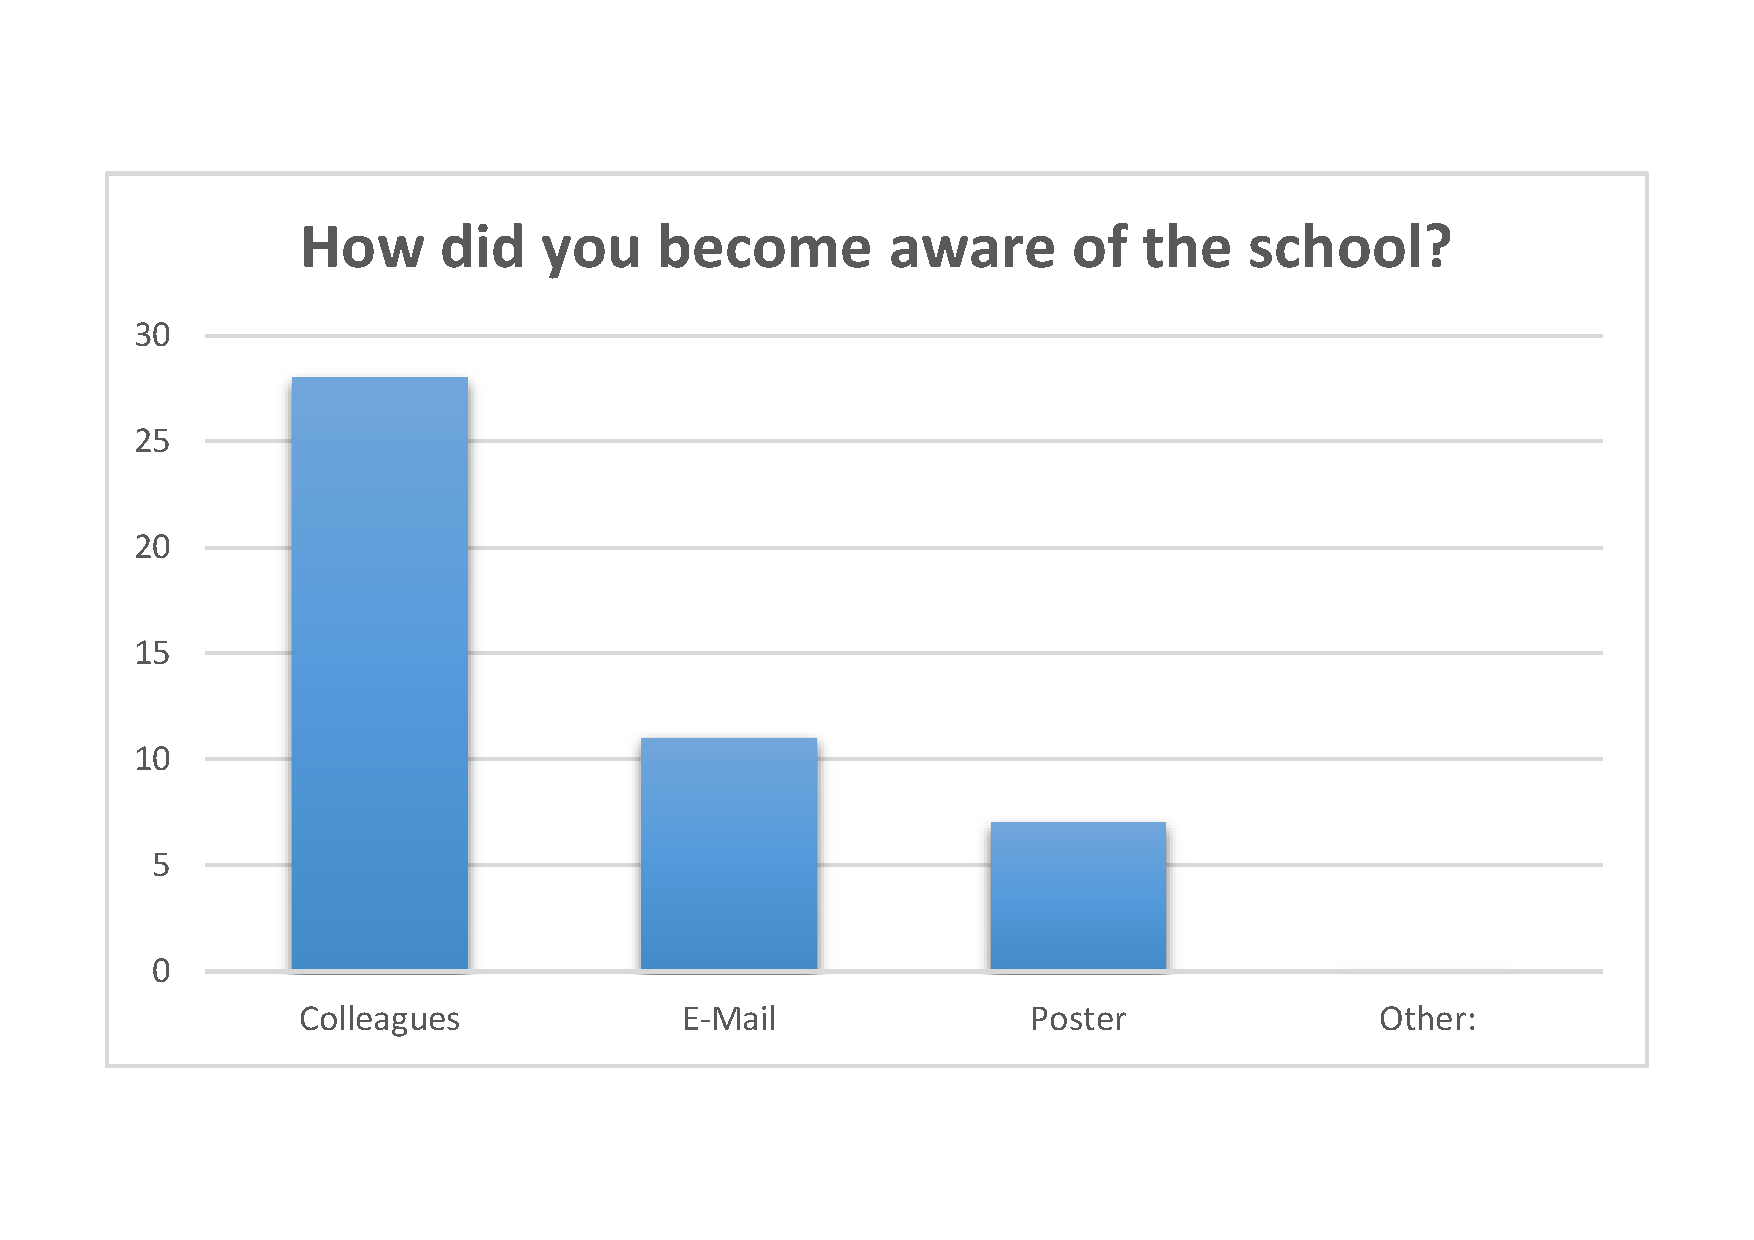
\includegraphics[width=0.8\textwidth]{eval/general/how_did_you_become_aware.pdf}
\caption{How did you become aware of the school? Multiple choices possible.}
\end{figure}
\begin{figure}[H]
\centering
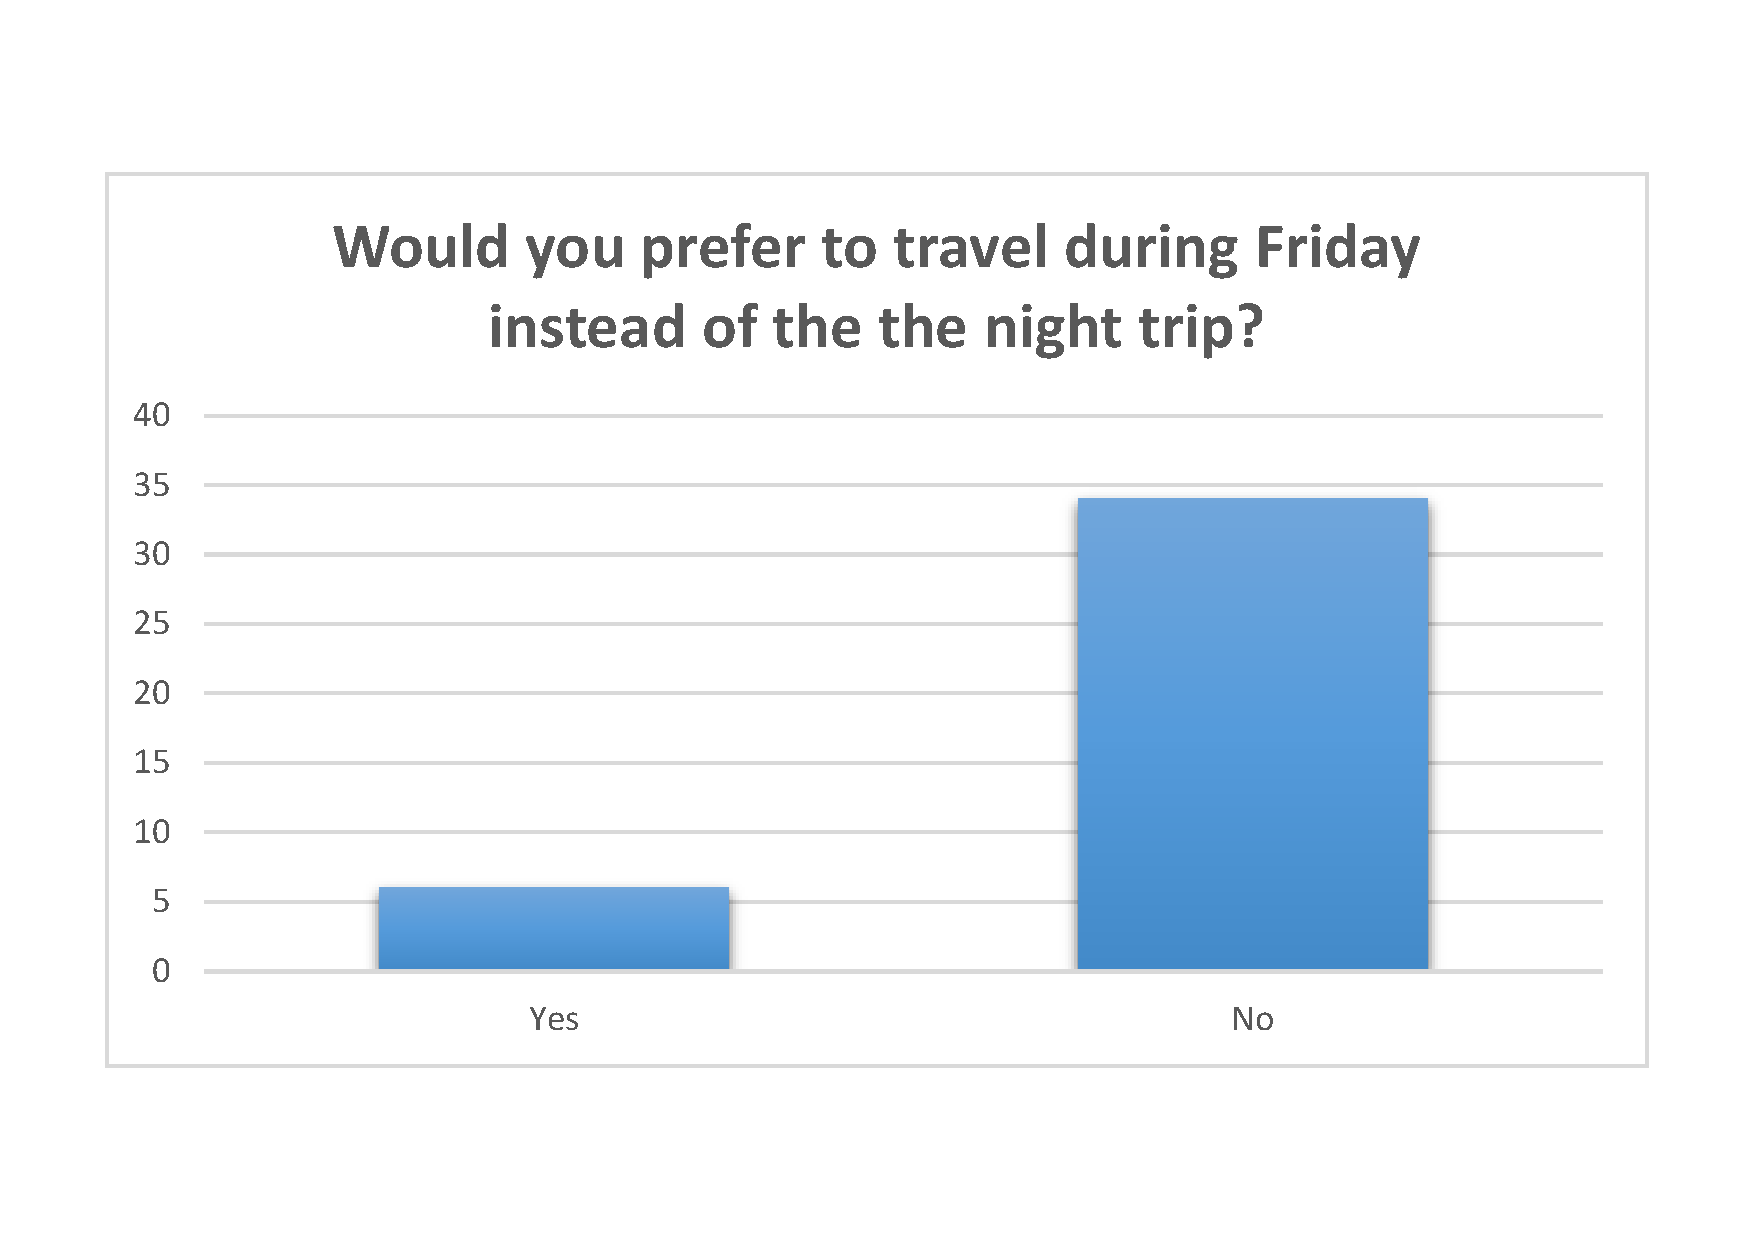
\includegraphics[width=0.8\textwidth]{eval/general/travel_per_night.pdf}
\caption{Would you have prefered to travel on Friday instead of the night trip and to arrive in Obergurgl on Friday evening?}
\end{figure}
\begin{figure}[H]
\centering
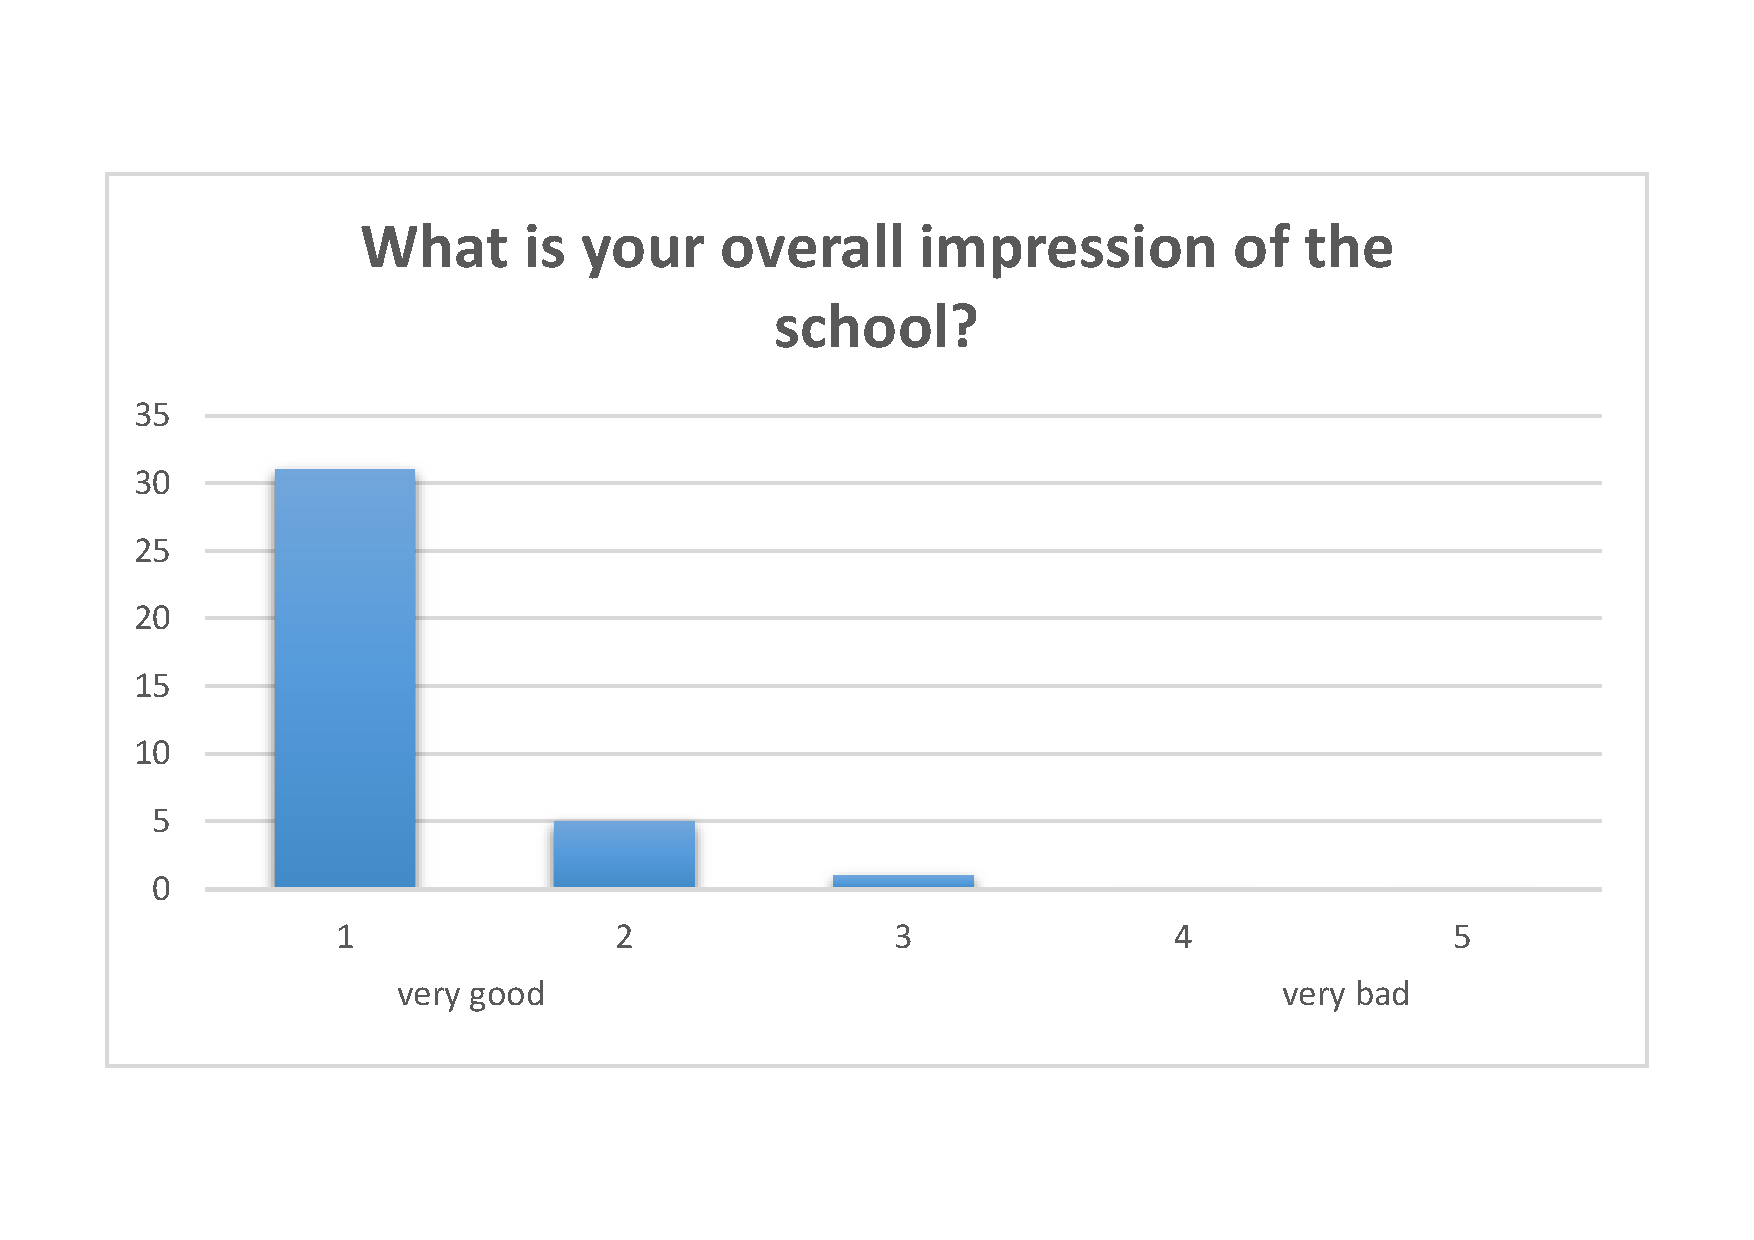
\includegraphics[width=0.8\textwidth]{eval/general/overall_impression.pdf}
\caption{What is your overall impression of the Winter School 2017?}
\end{figure}


\begin{figure}[H]
\centering
\null\hfill %
\subfloat[\label{a}]{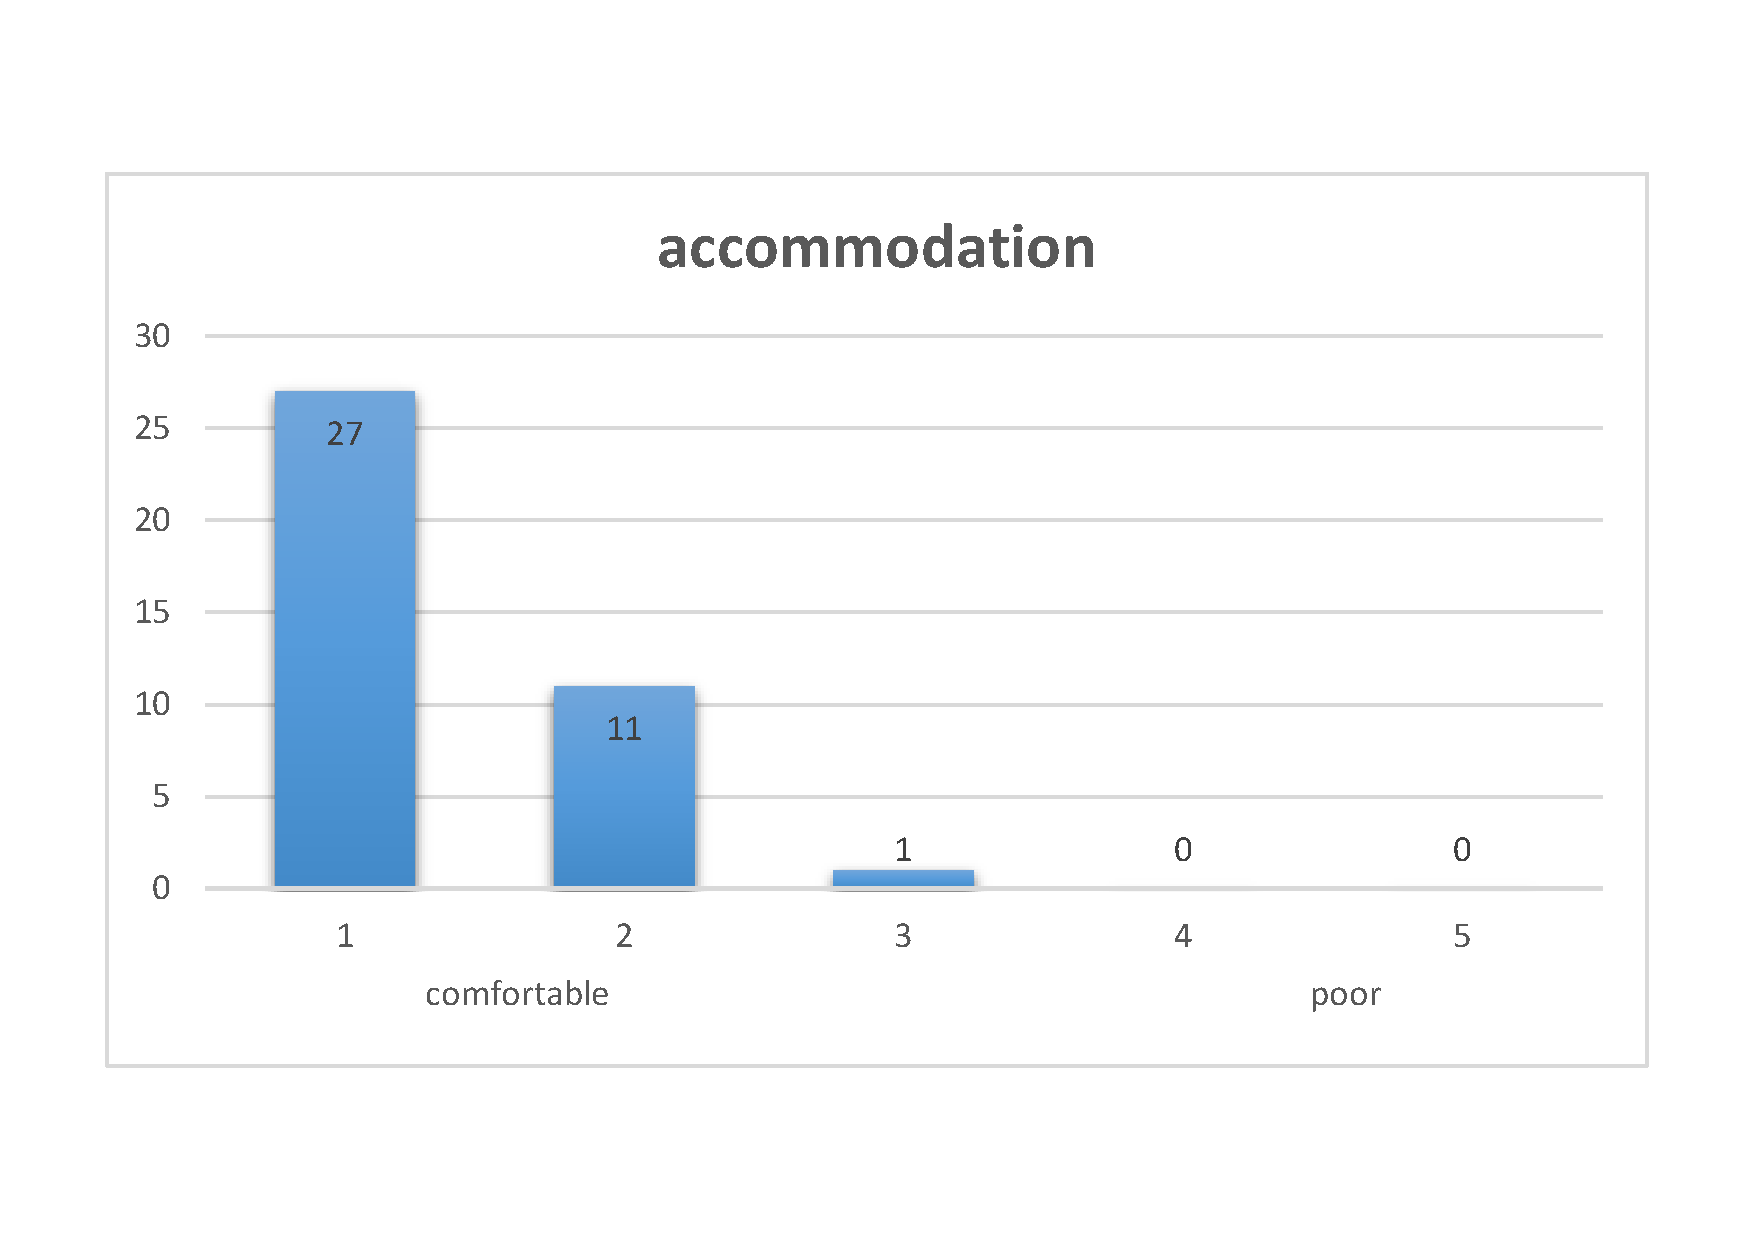
\includegraphics[width=0.5\textwidth]{eval/general/accommodation.pdf}}
\hfill %
\subfloat[\label{b}]{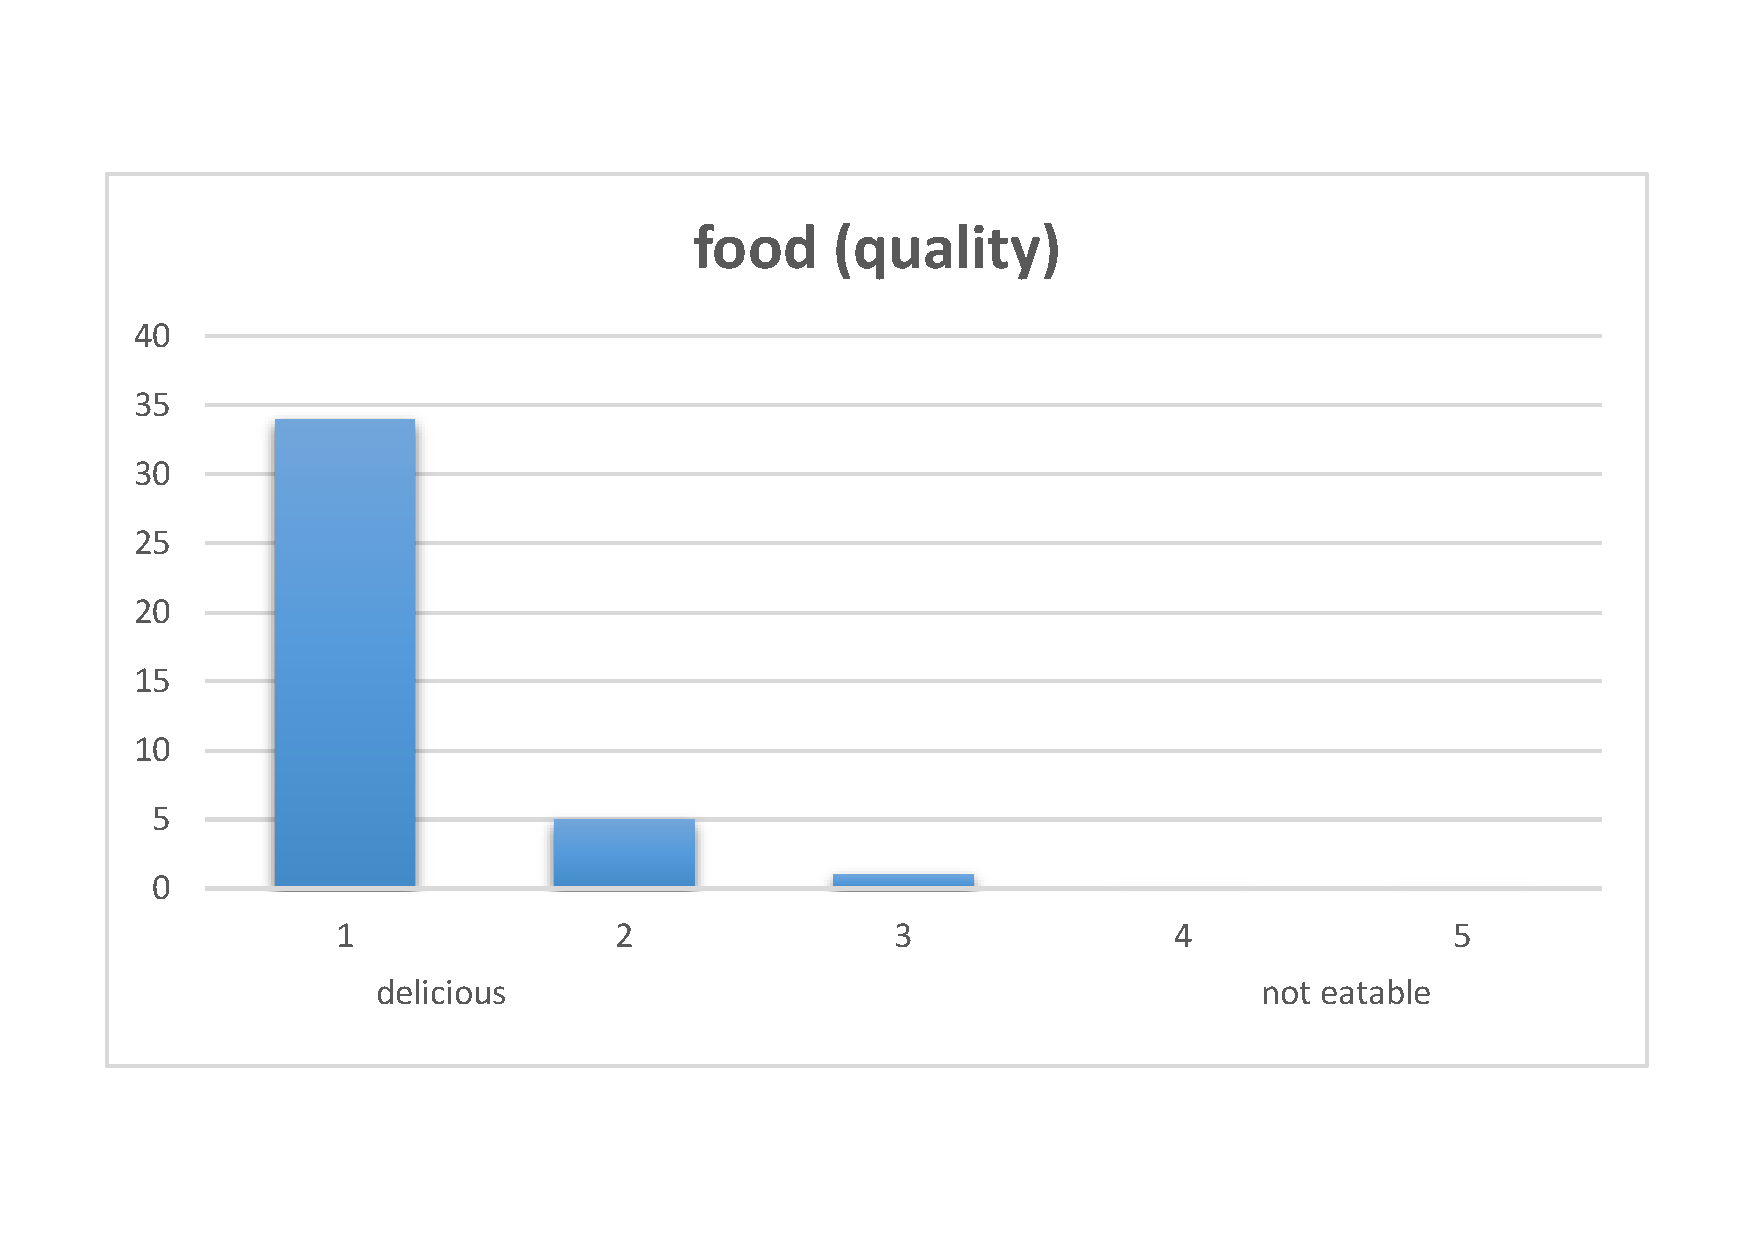
\includegraphics[width=0.5\textwidth]{eval/general/food_quality.pdf}}
\hfill %
\subfloat[\label{b}]{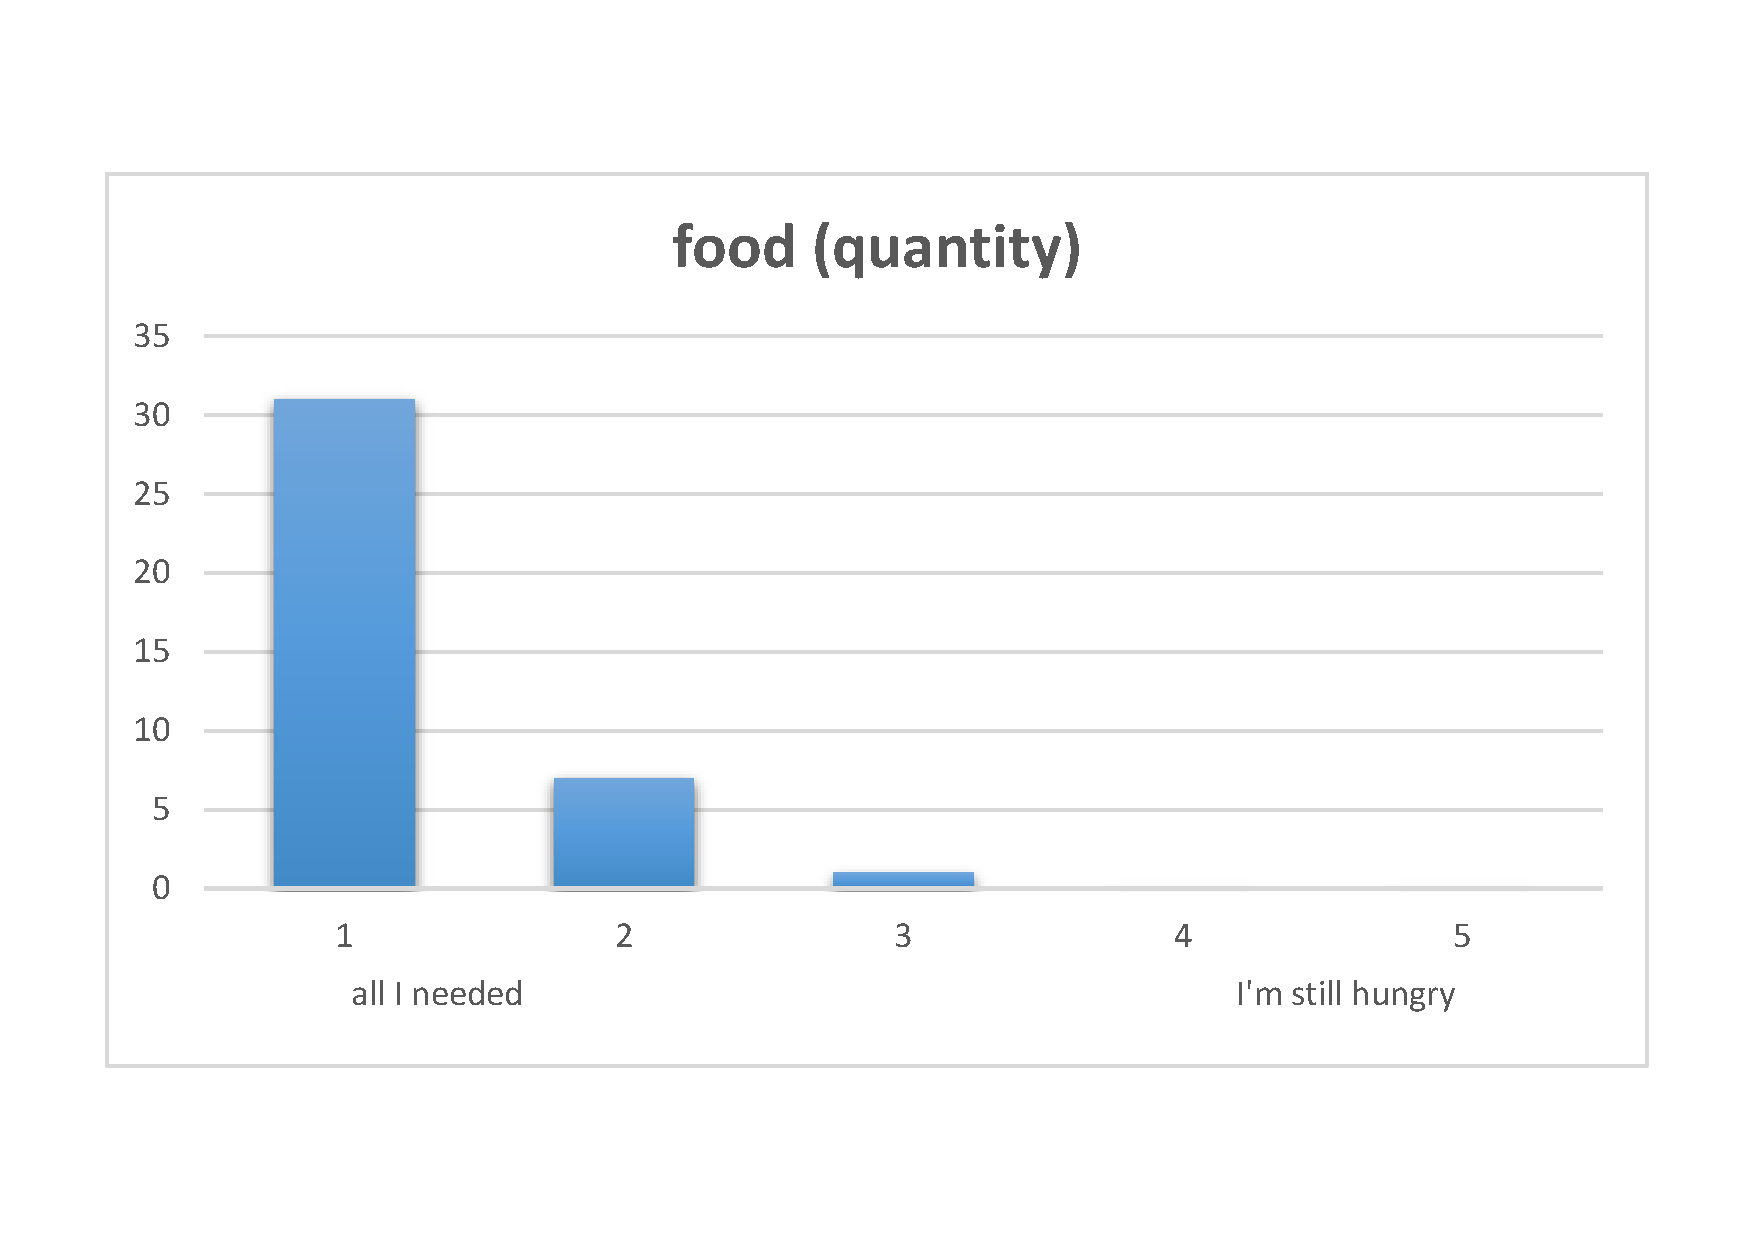
\includegraphics[width=0.5\textwidth]{eval/general/food_quantity.pdf}}
\hfill %
\subfloat[\label{b}]{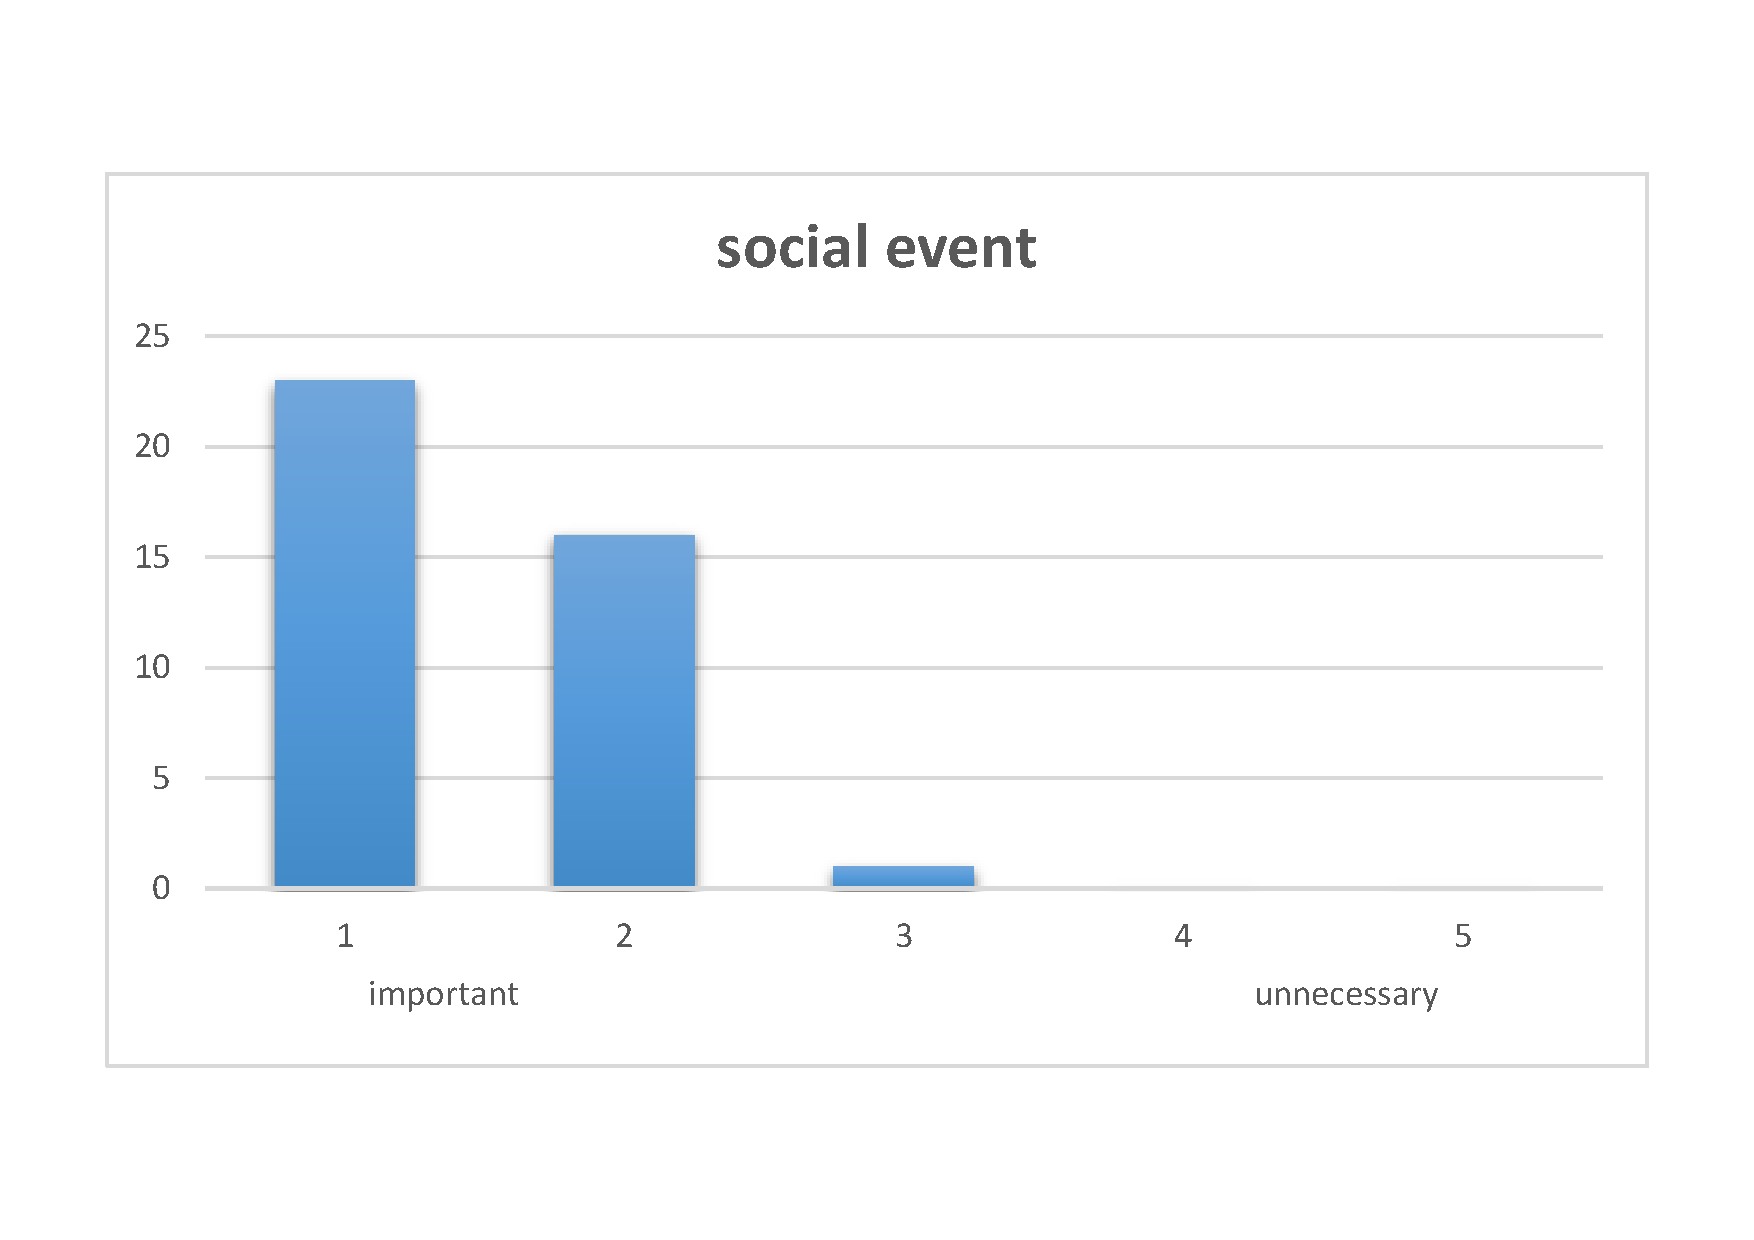
\includegraphics[width=0.5\textwidth]{eval/general/social_event.pdf}}
\hfill %
\subfloat[\label{b}]{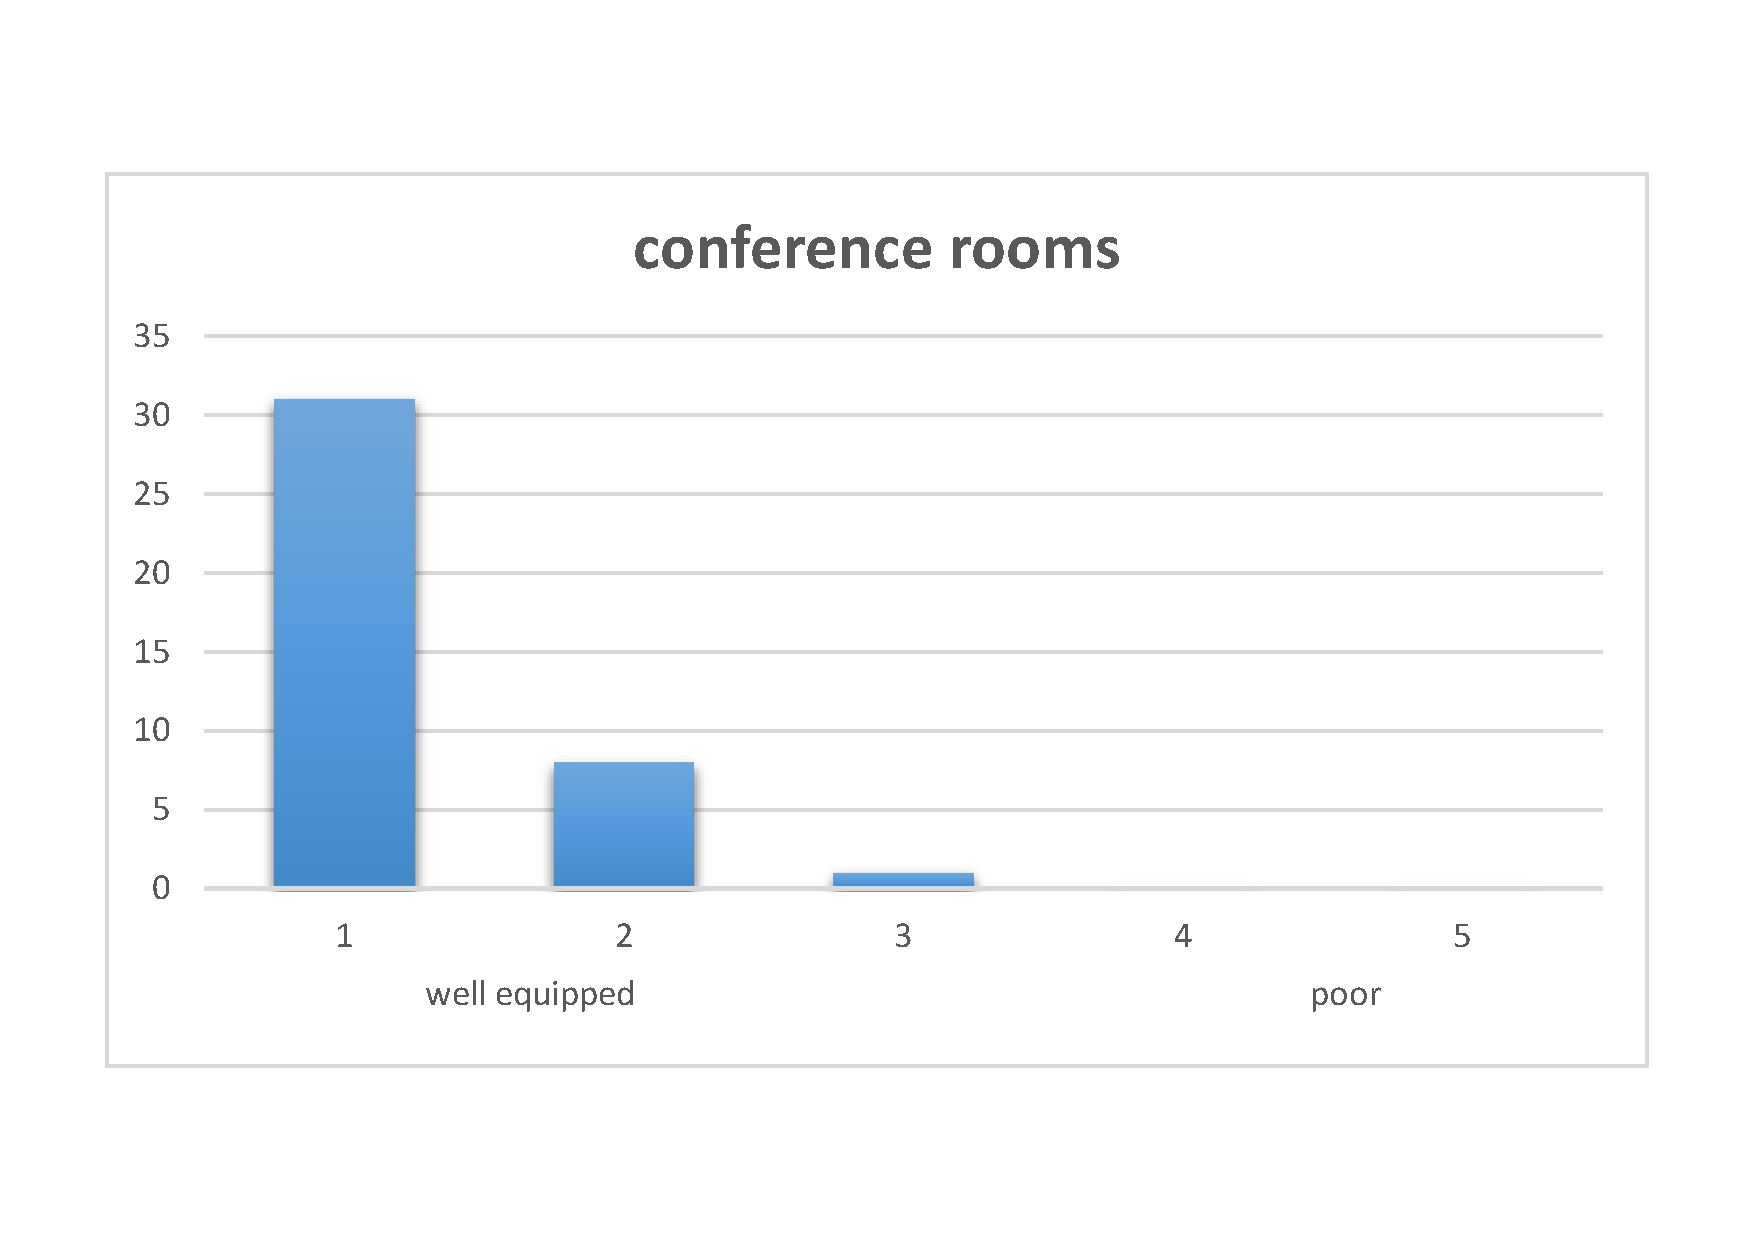
\includegraphics[width=0.5\textwidth]{eval/general/conference_rooms.pdf}}
\hfill %
\subfloat[\label{b}]{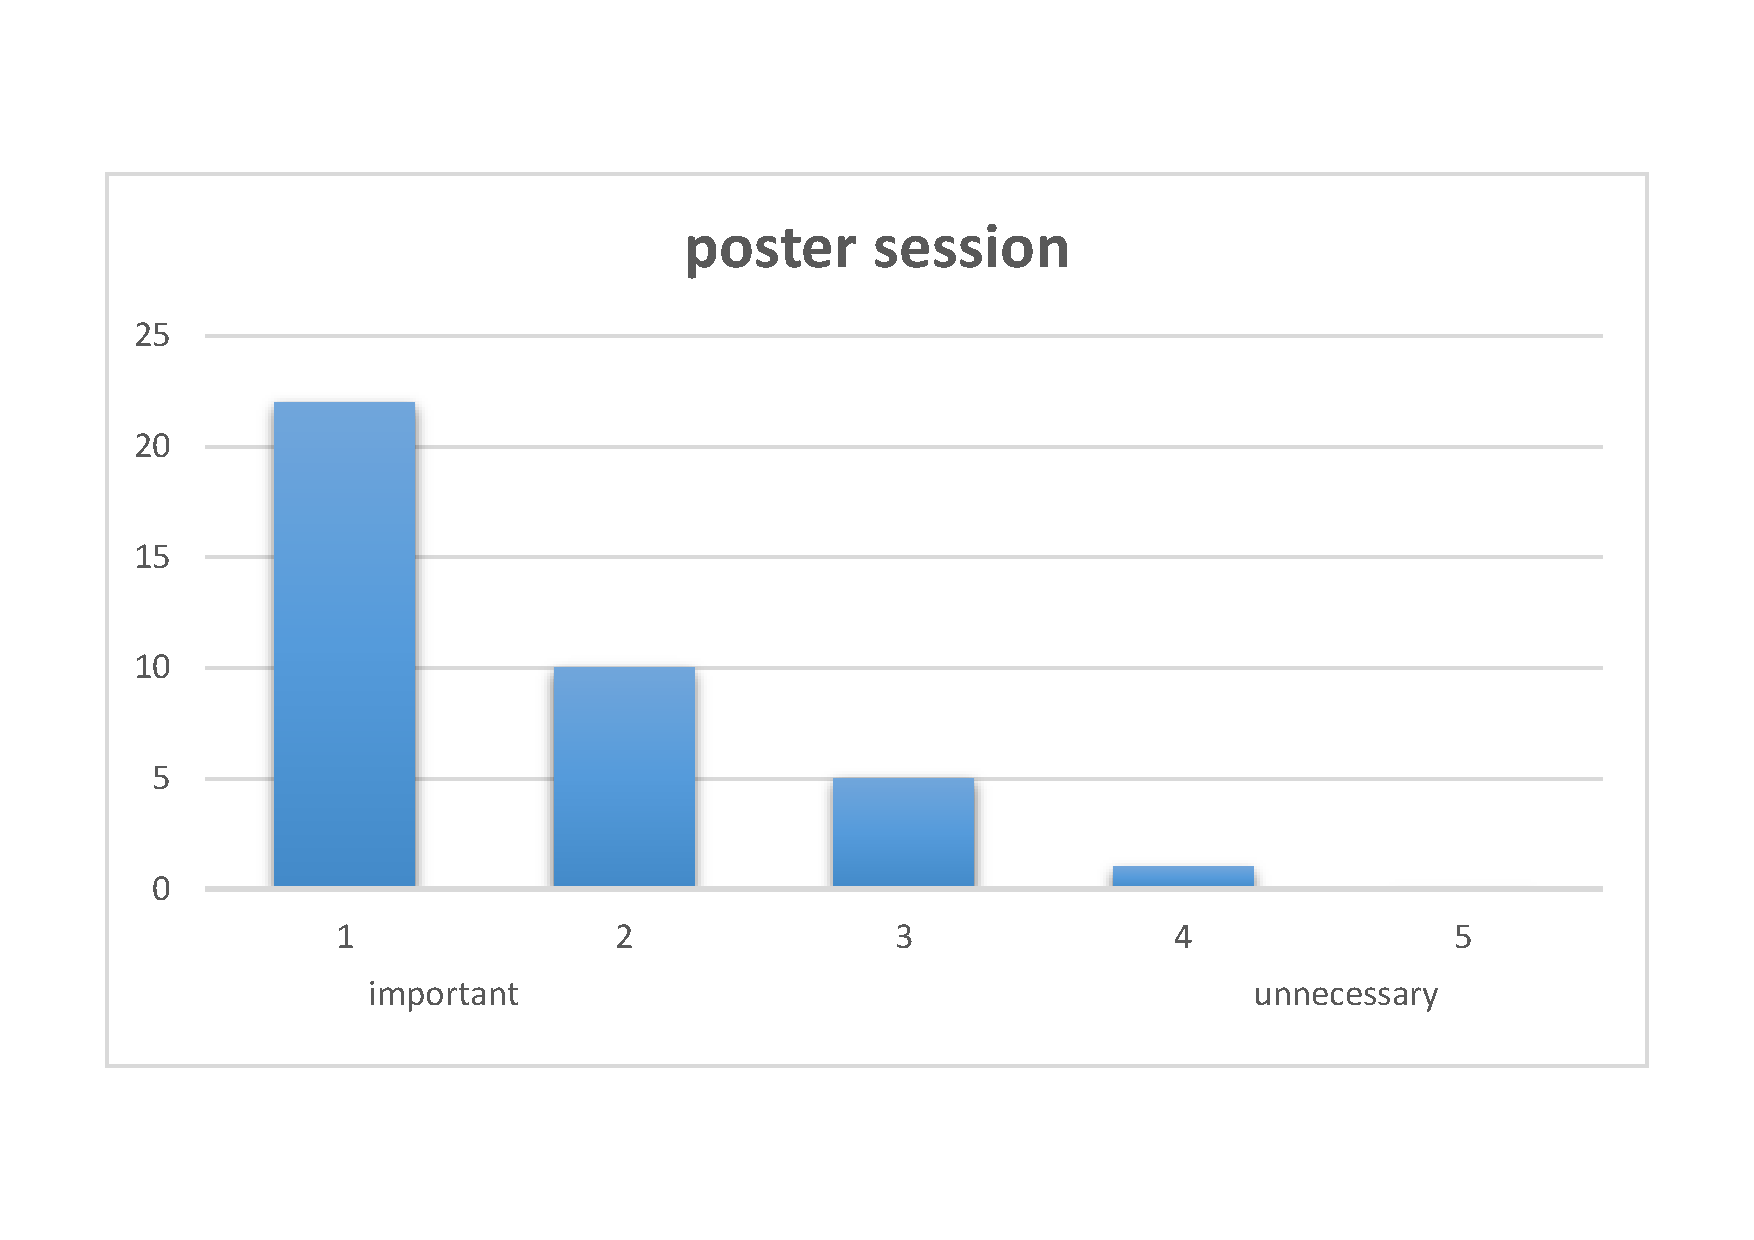
\includegraphics[width=0.5\textwidth]{eval/general/poster_session.pdf}}
\hfill\null % 
\caption{General evaluation of the winterschool (part 1)}
\end{figure}  

\begin{figure}[H]
\centering
\null\hfill %
\subfloat[\label{b}]{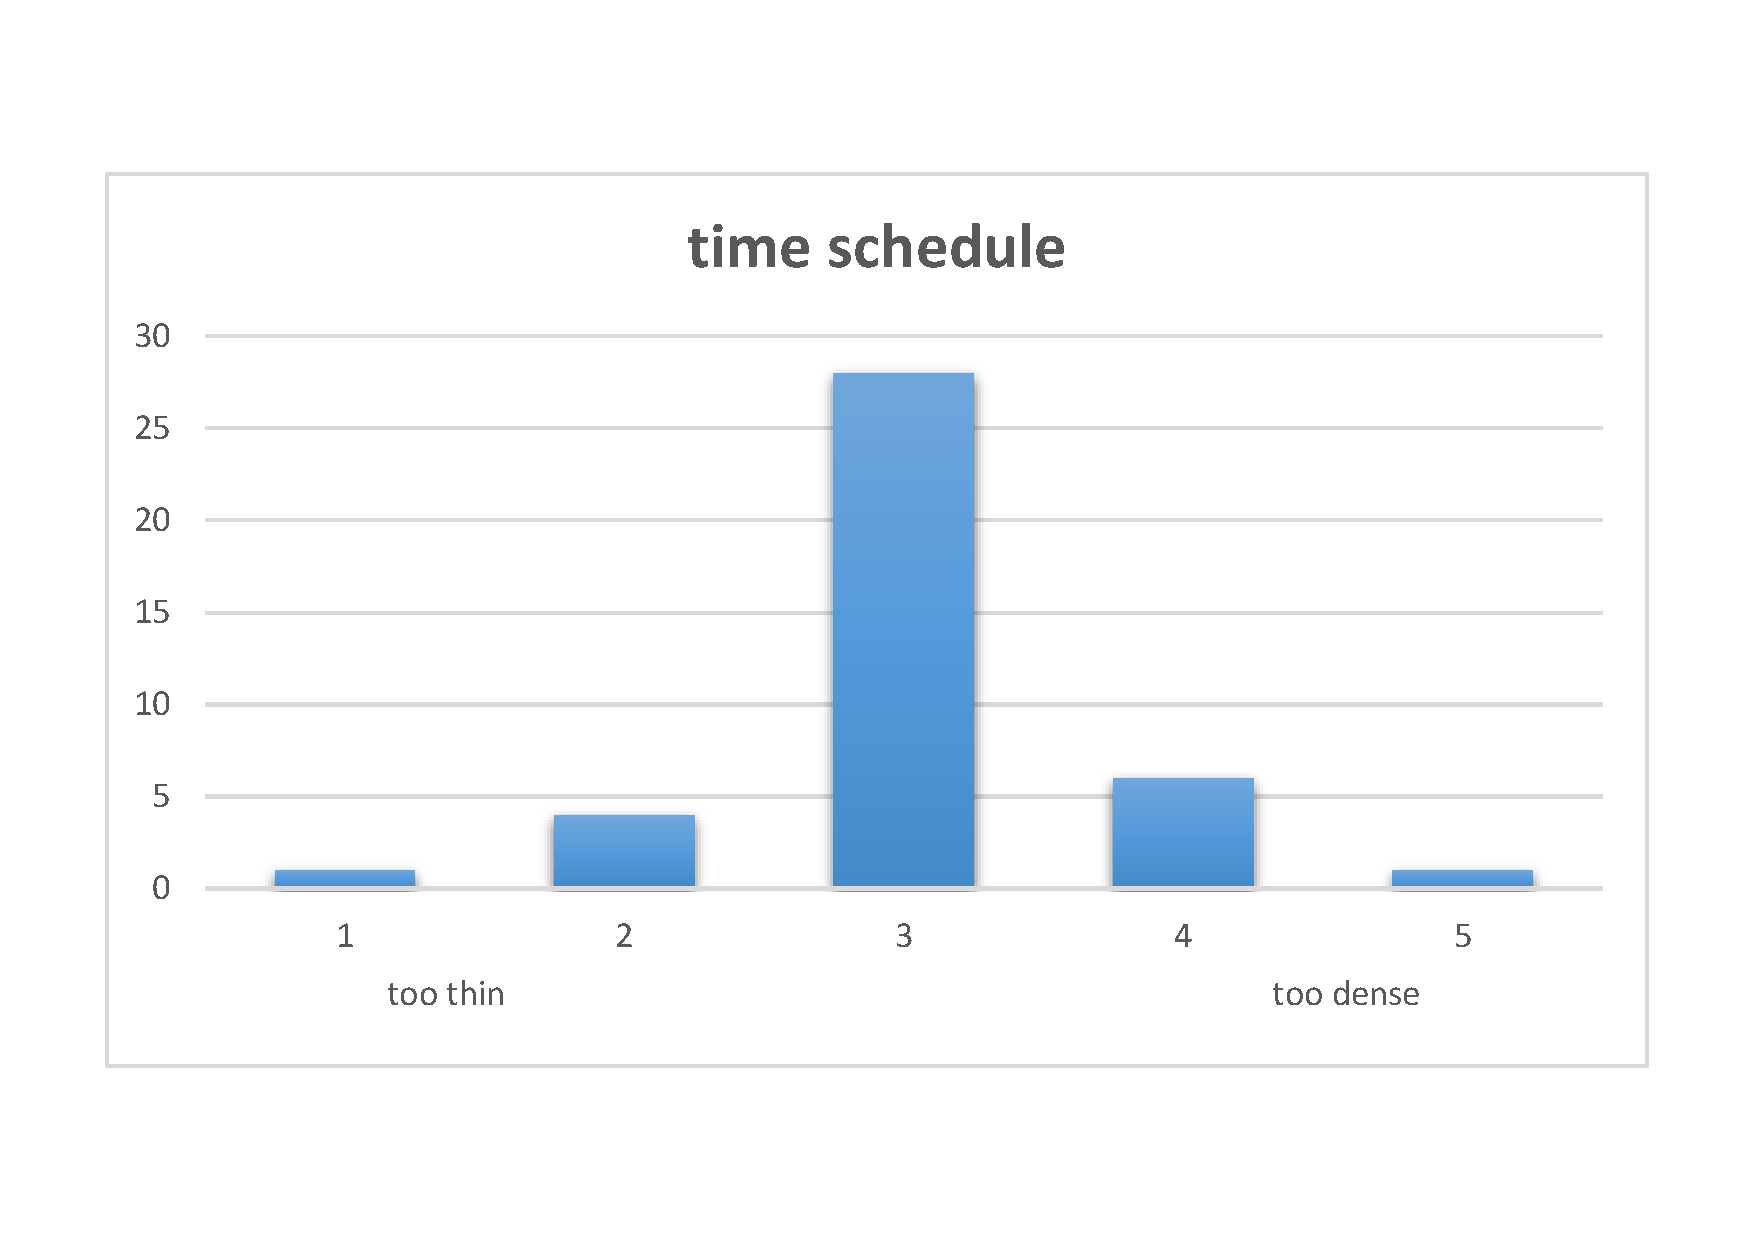
\includegraphics[width=0.5\textwidth]{eval/general/schedule.pdf}}
\hfill %
\subfloat[\label{b}]{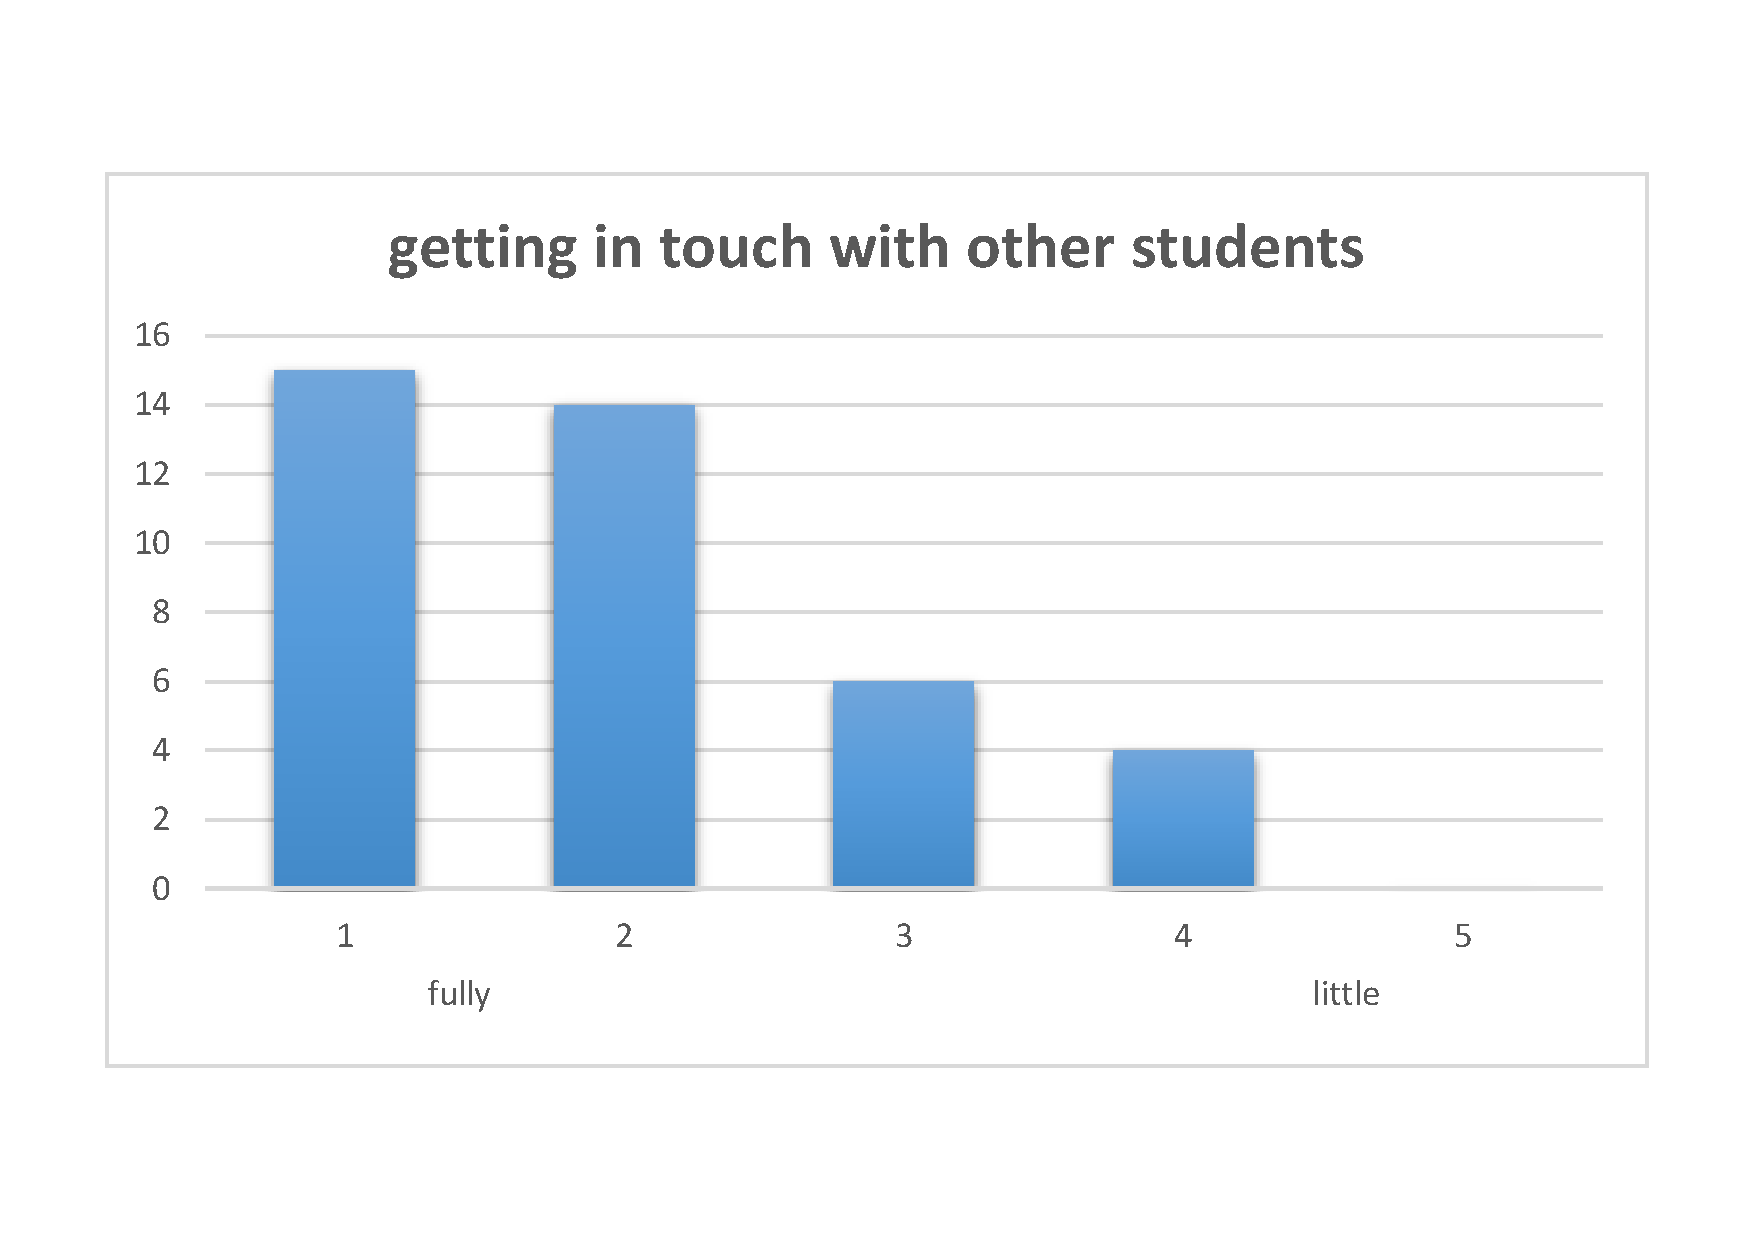
\includegraphics[width=0.5\textwidth]{eval/general/getting_in_touch.pdf}}
\hfill %
\subfloat[\label{b}]{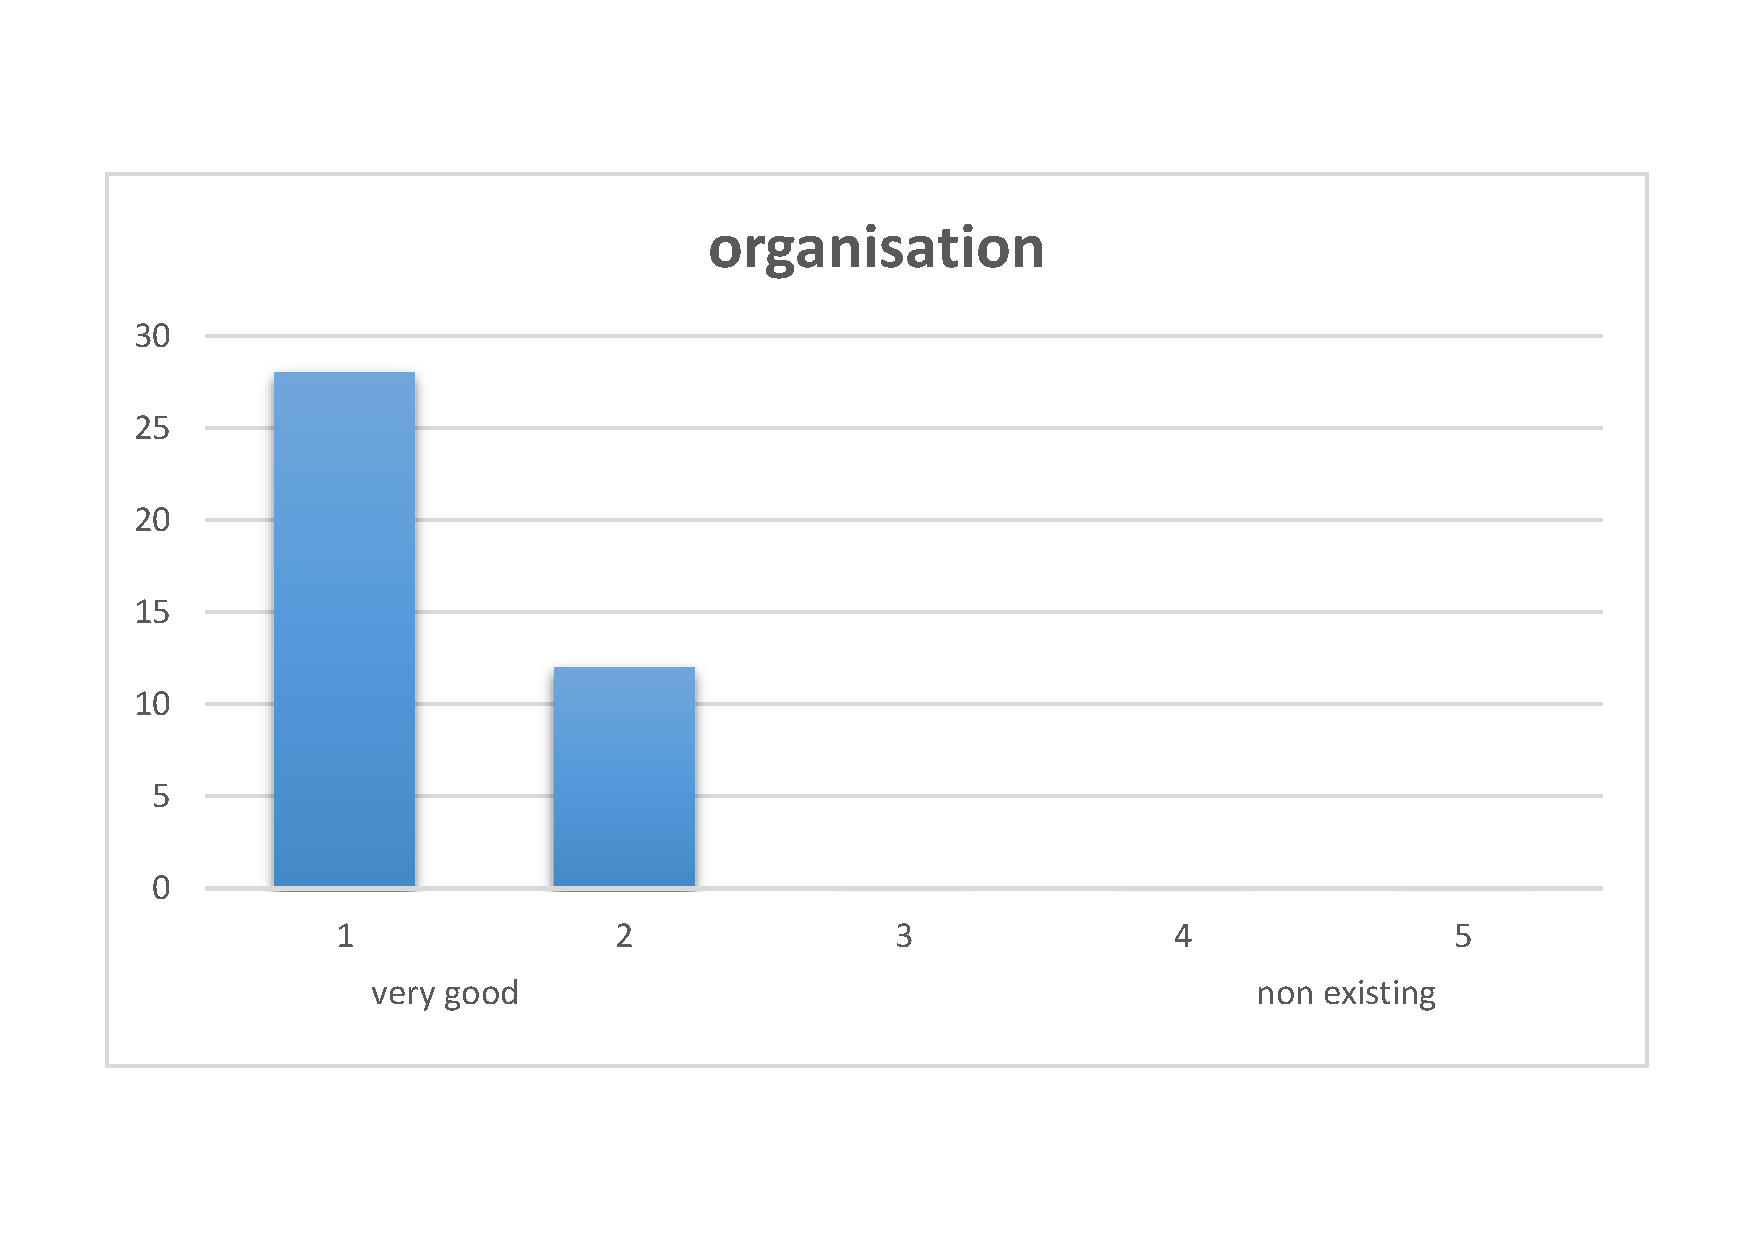
\includegraphics[width=0.5\textwidth]{eval/general/organisation.pdf}}
\hfill\null % 
\caption{General evaluation of the winterschool (part 2)}
\end{figure} 

\subsection{Lecture evaluations}

\subsubsection{Invitation Lecture: M. Dunford  - "From riots to raves"}

\begin{figure}[H]
\centering
\null\hfill %
\subfloat[\label{b}]{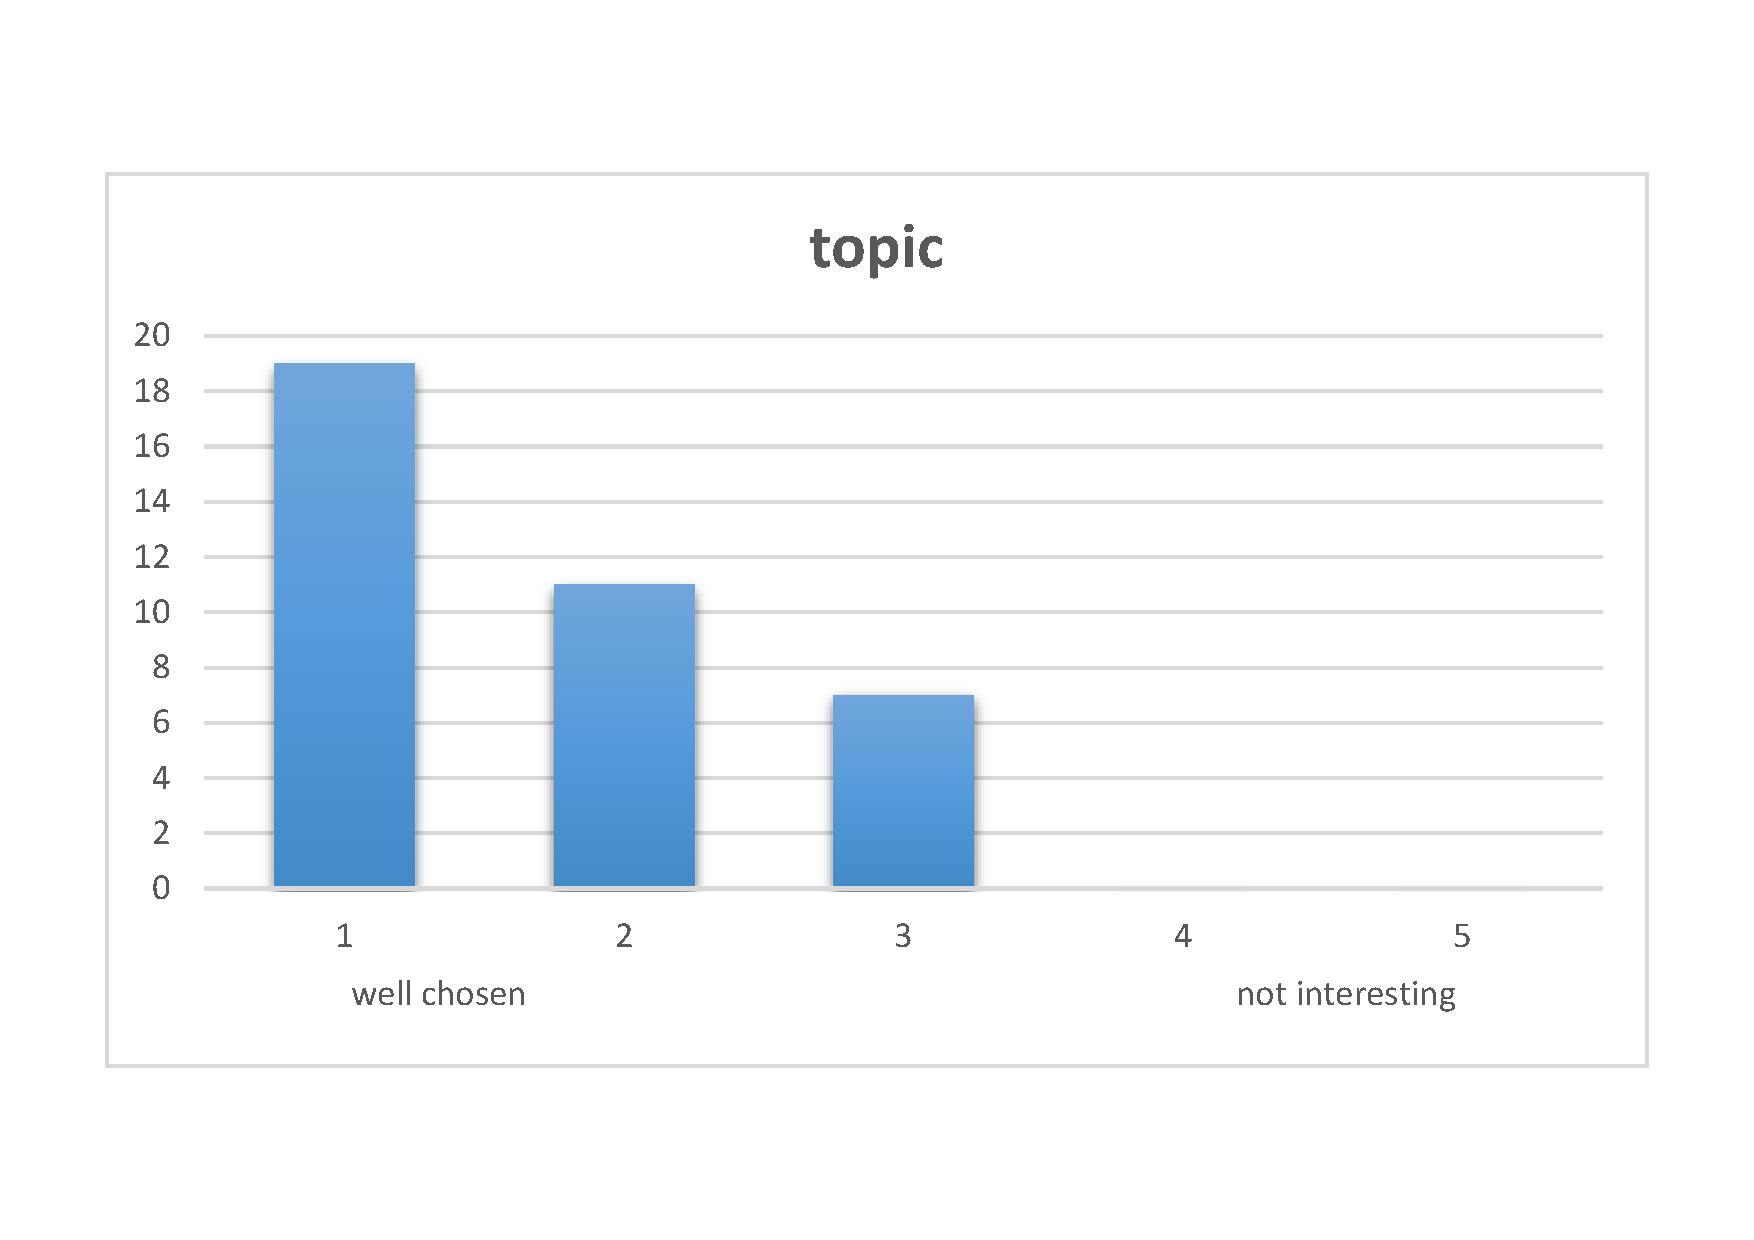
\includegraphics[width=0.5\textwidth]{eval/dunford/topic.pdf}}
\hfill %
\subfloat[\label{b}]{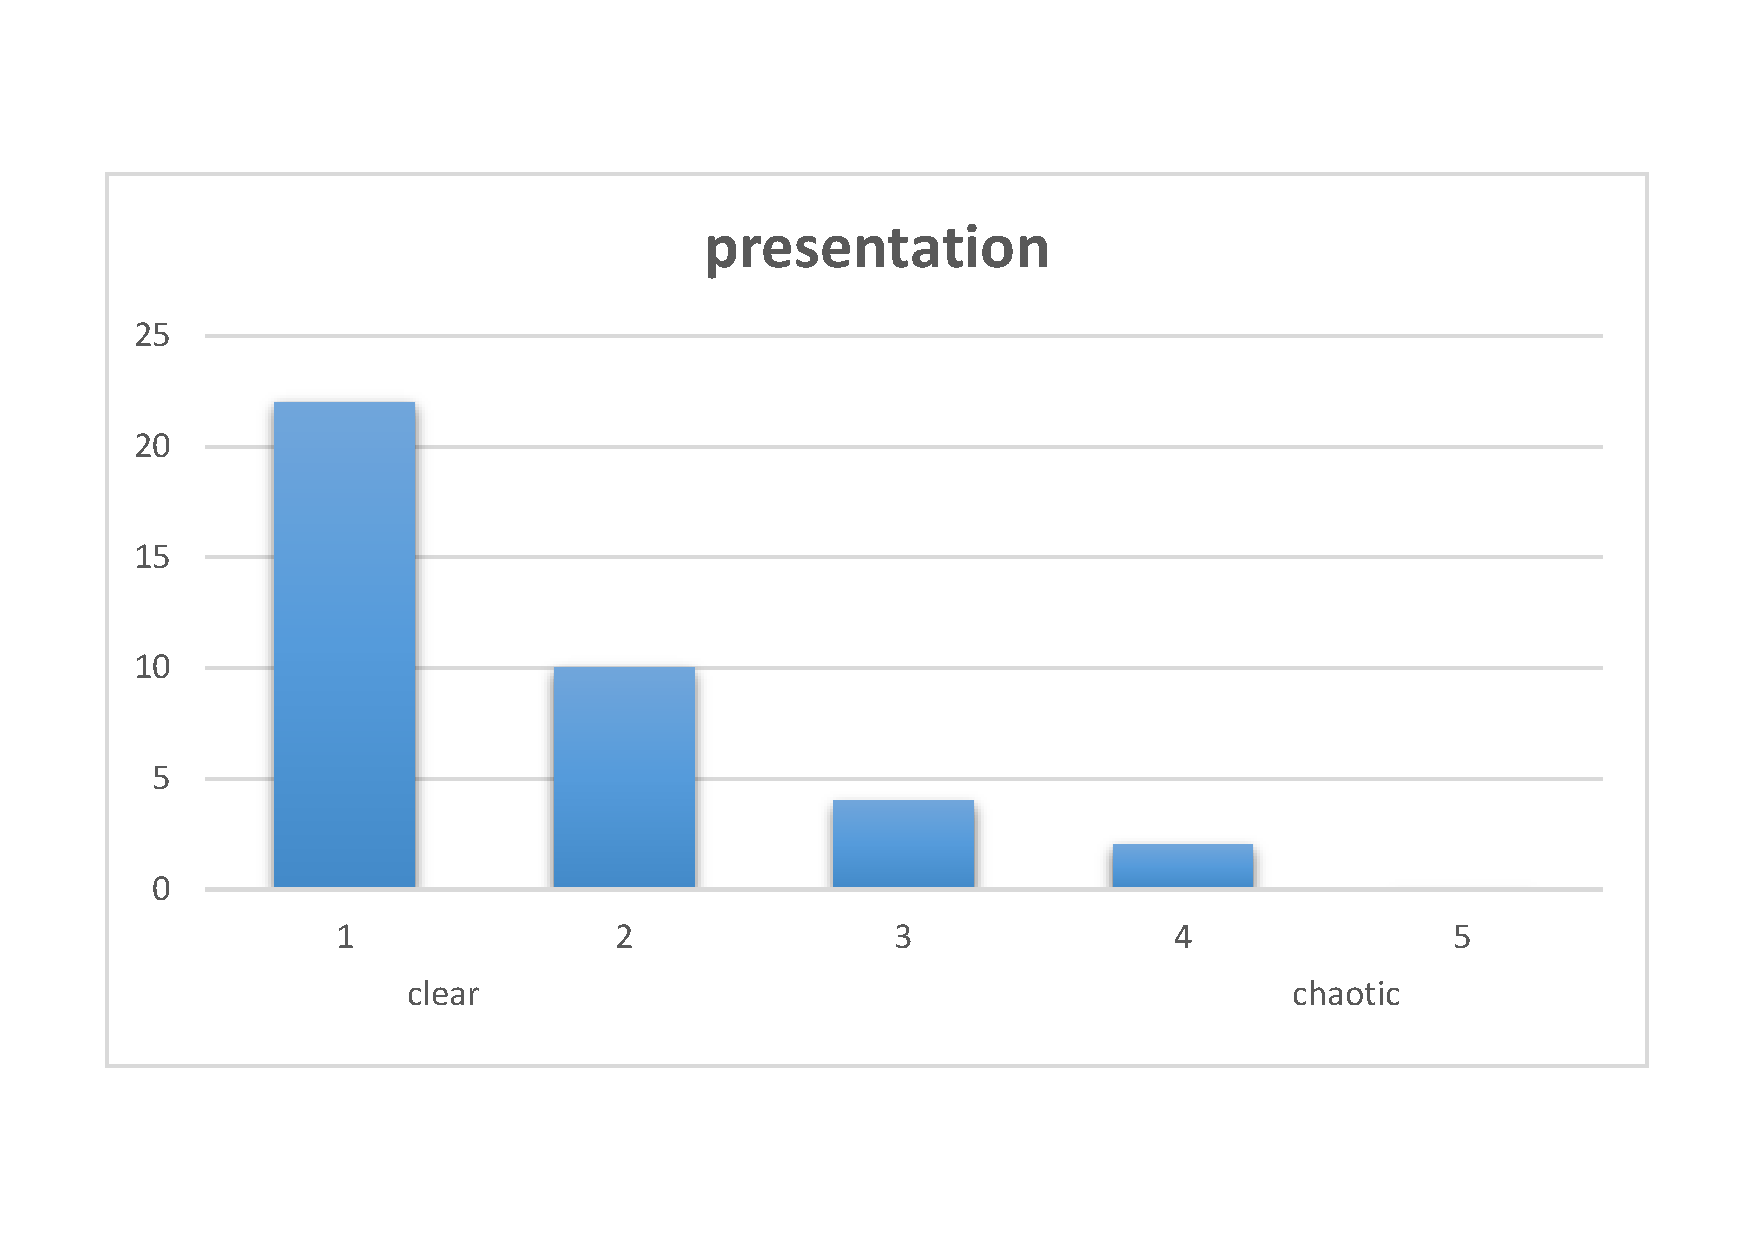
\includegraphics[width=0.5\textwidth]{eval/dunford/presentation.pdf}}
\hfill %
\subfloat[\label{b}]{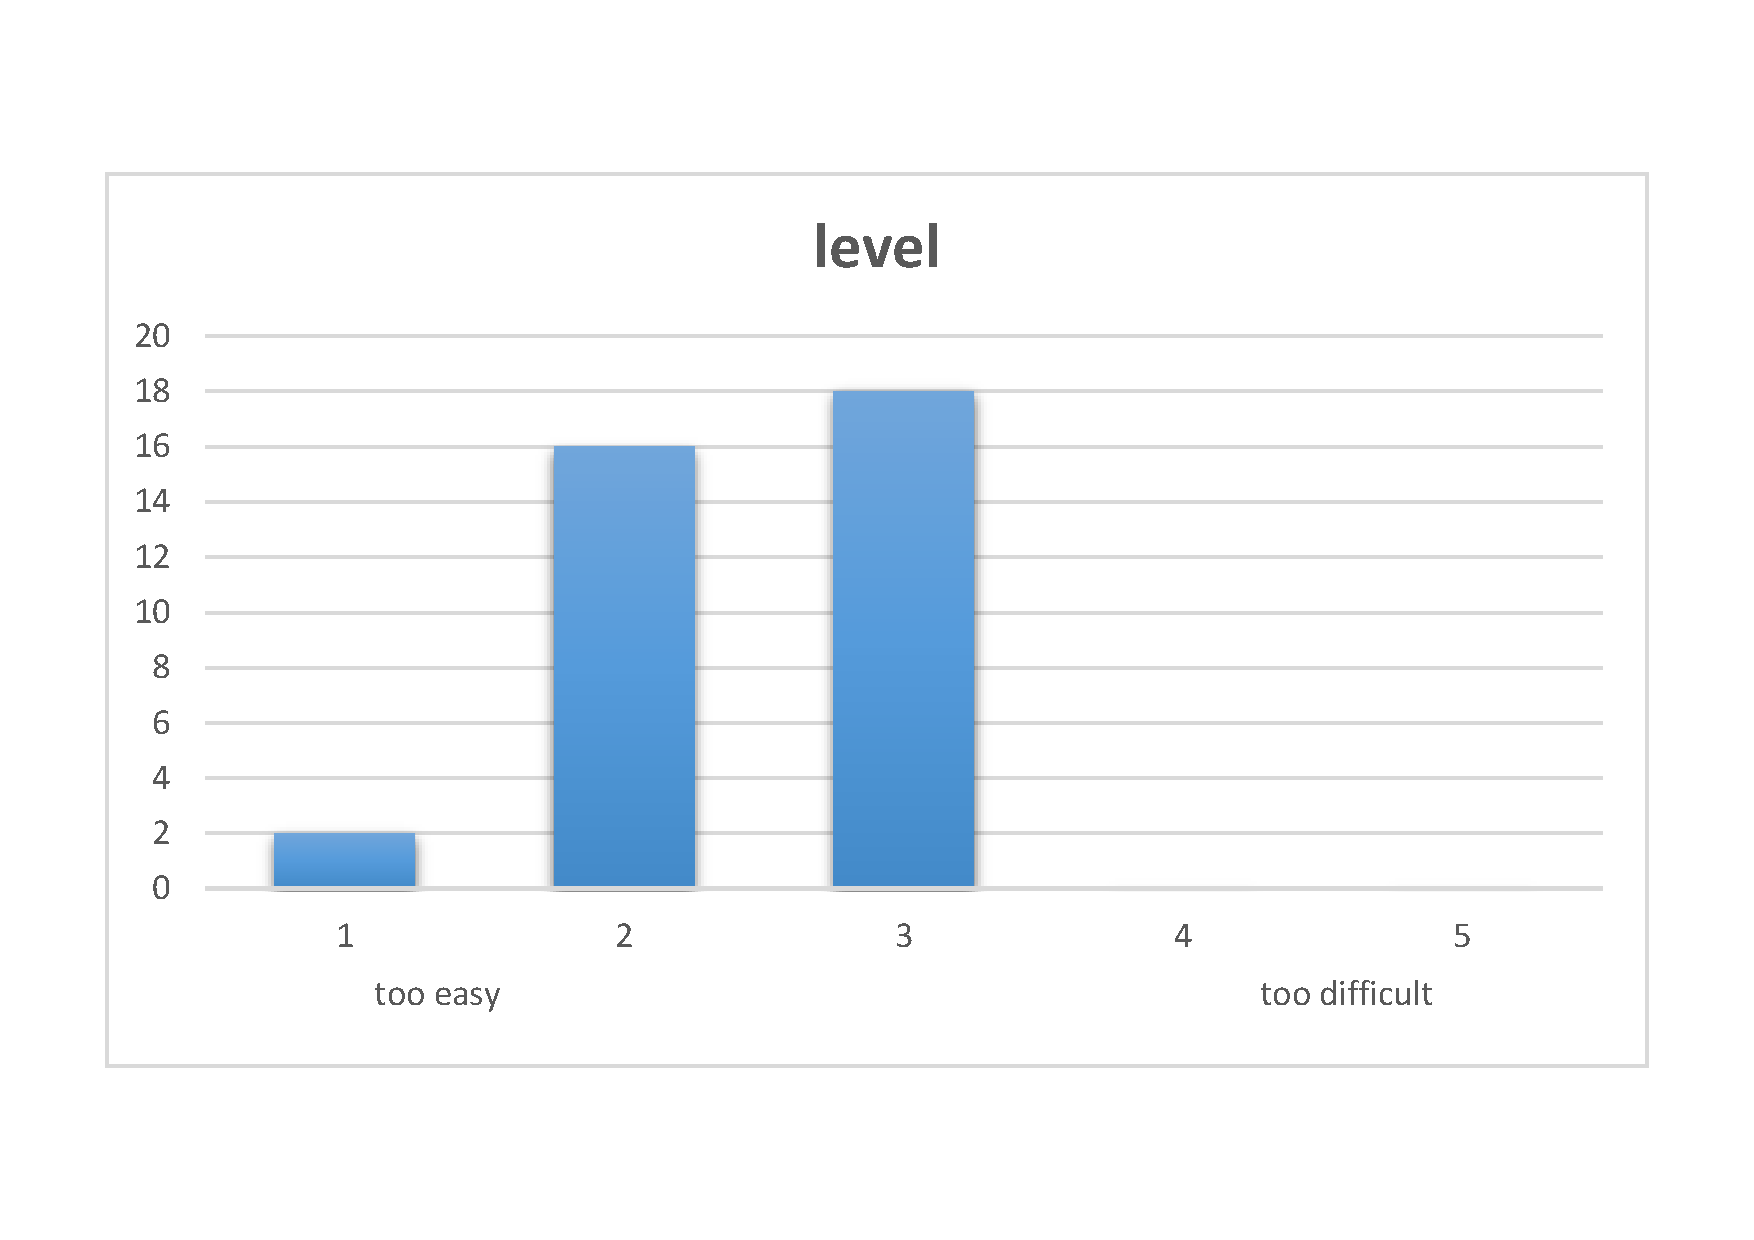
\includegraphics[width=0.5\textwidth]{eval/dunford/level.pdf}}
\hfill %
\subfloat[\label{b}]{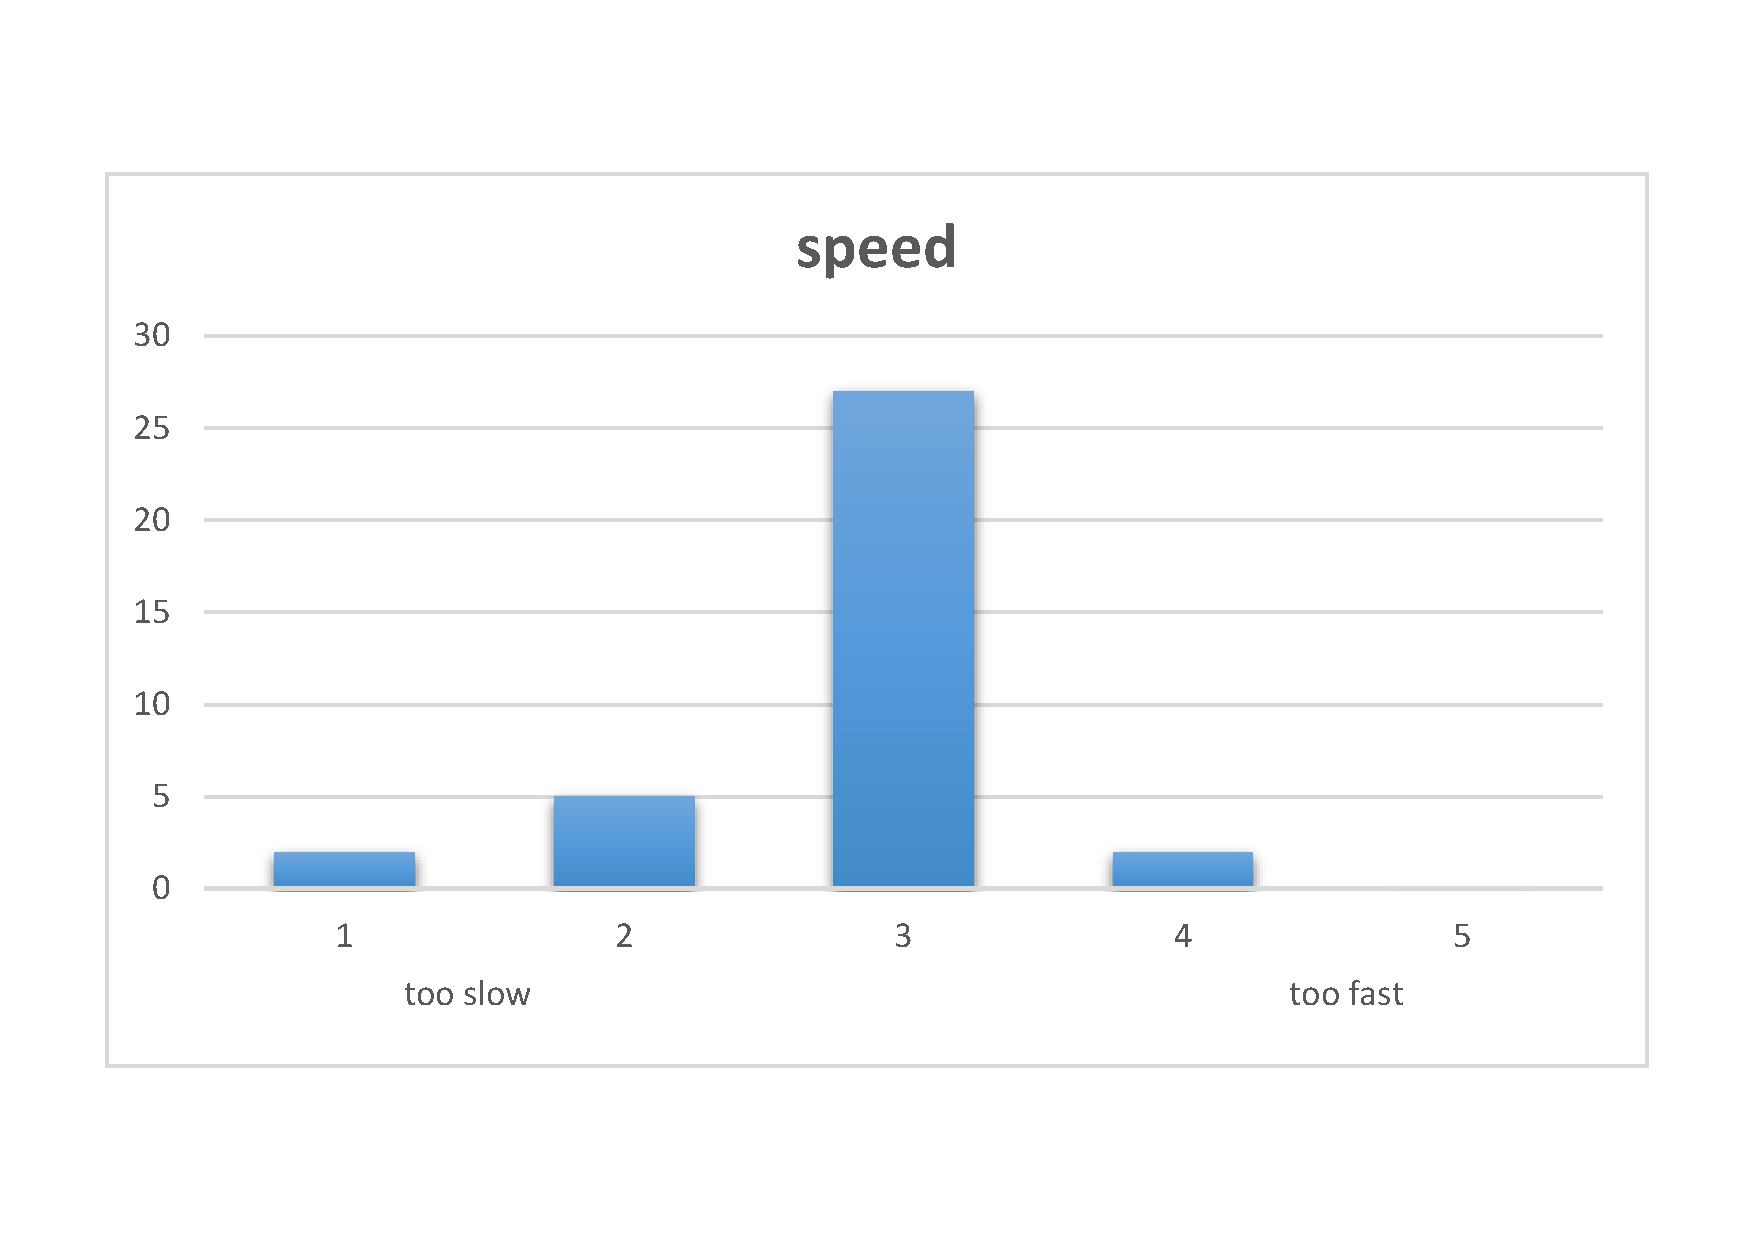
\includegraphics[width=0.5\textwidth]{eval/dunford/speed.pdf}}
\hfill\null % 
\caption{Invitation Lecture: M. Dunford - "From riots to raves"}
\end{figure} 

\subsubsection{Lecture: C. F. Anders  - "Jets to the future: Boosted boson and top jets as a probe for new physics"}

\begin{figure}[H]
\centering
\null\hfill %
\subfloat[\label{b}]{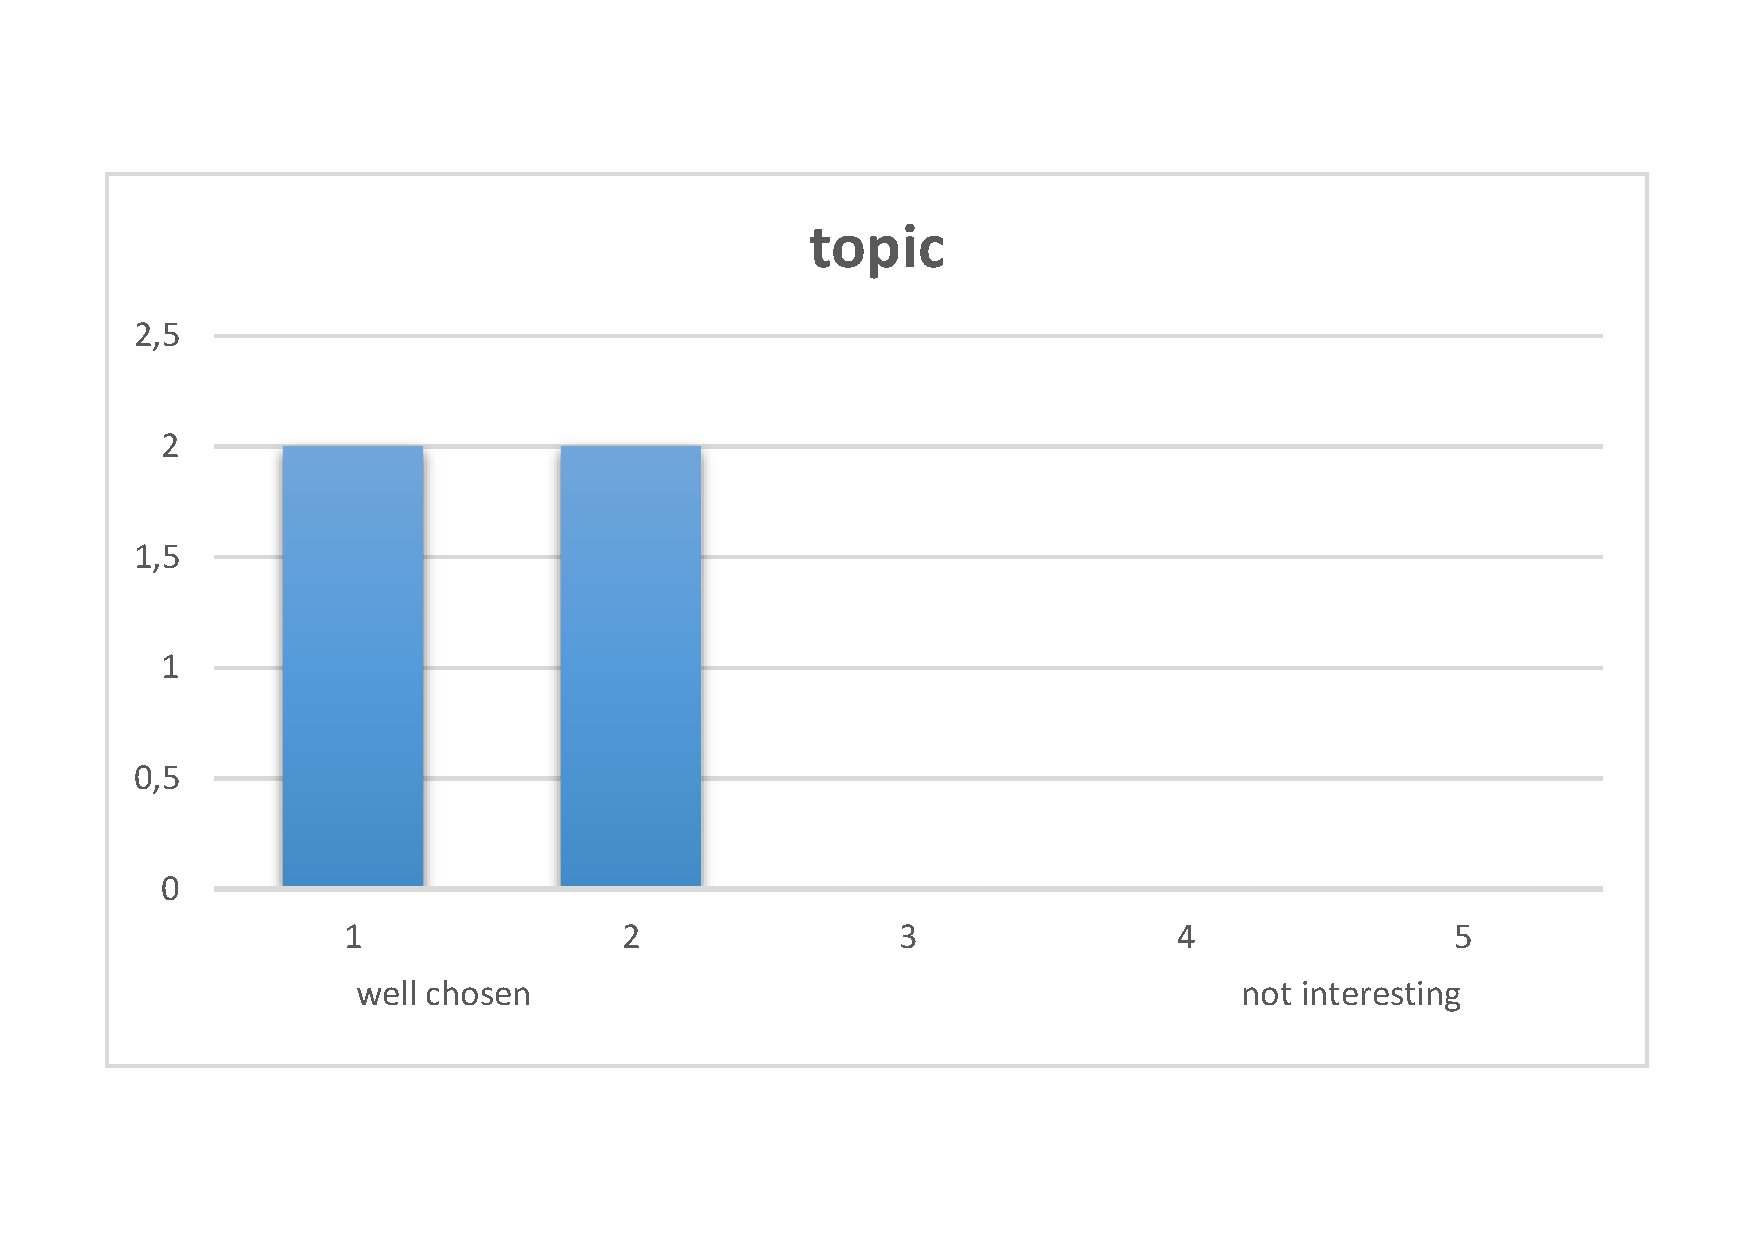
\includegraphics[width=0.5\textwidth]{eval/anders/topic.pdf}}
\hfill %
\subfloat[\label{b}]{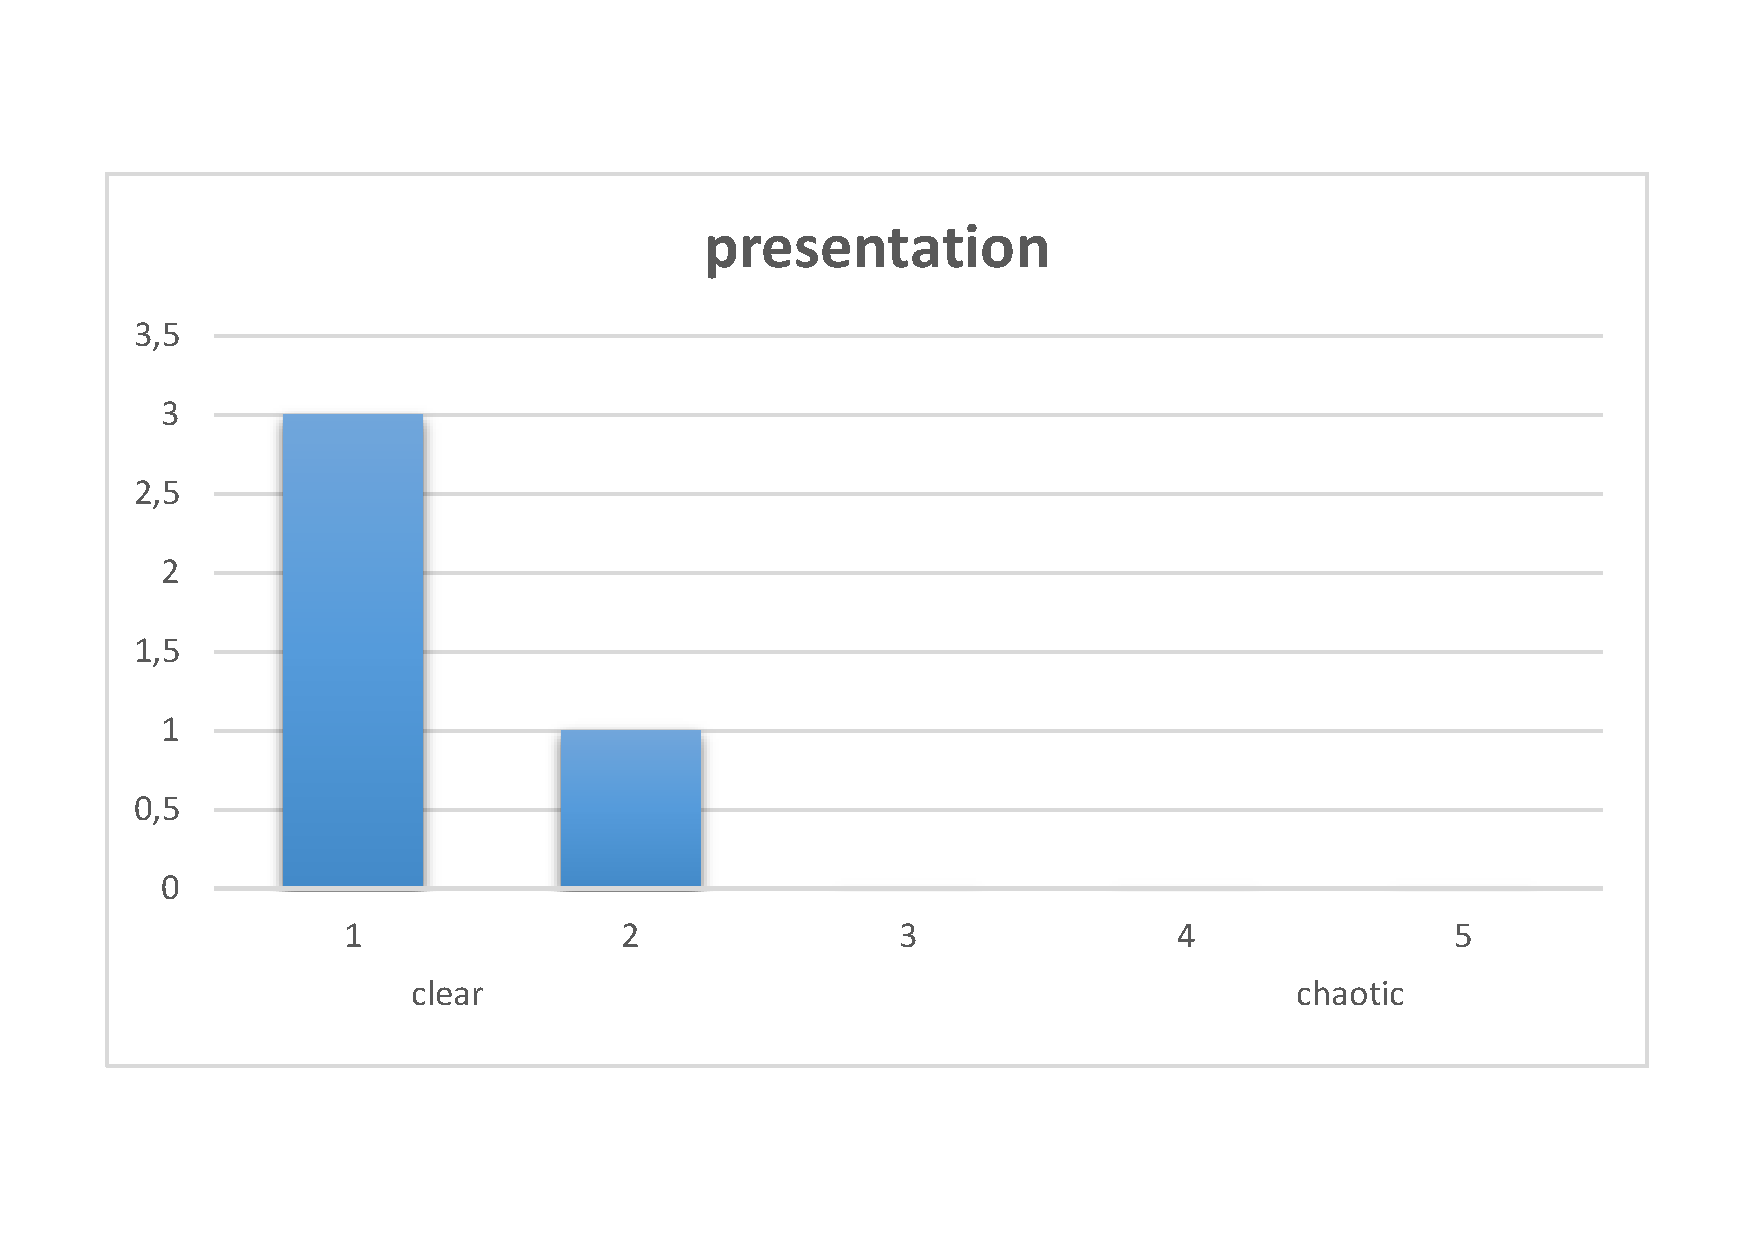
\includegraphics[width=0.5\textwidth]{eval/anders/presentation.pdf}}
\hfill %
\subfloat[\label{b}]{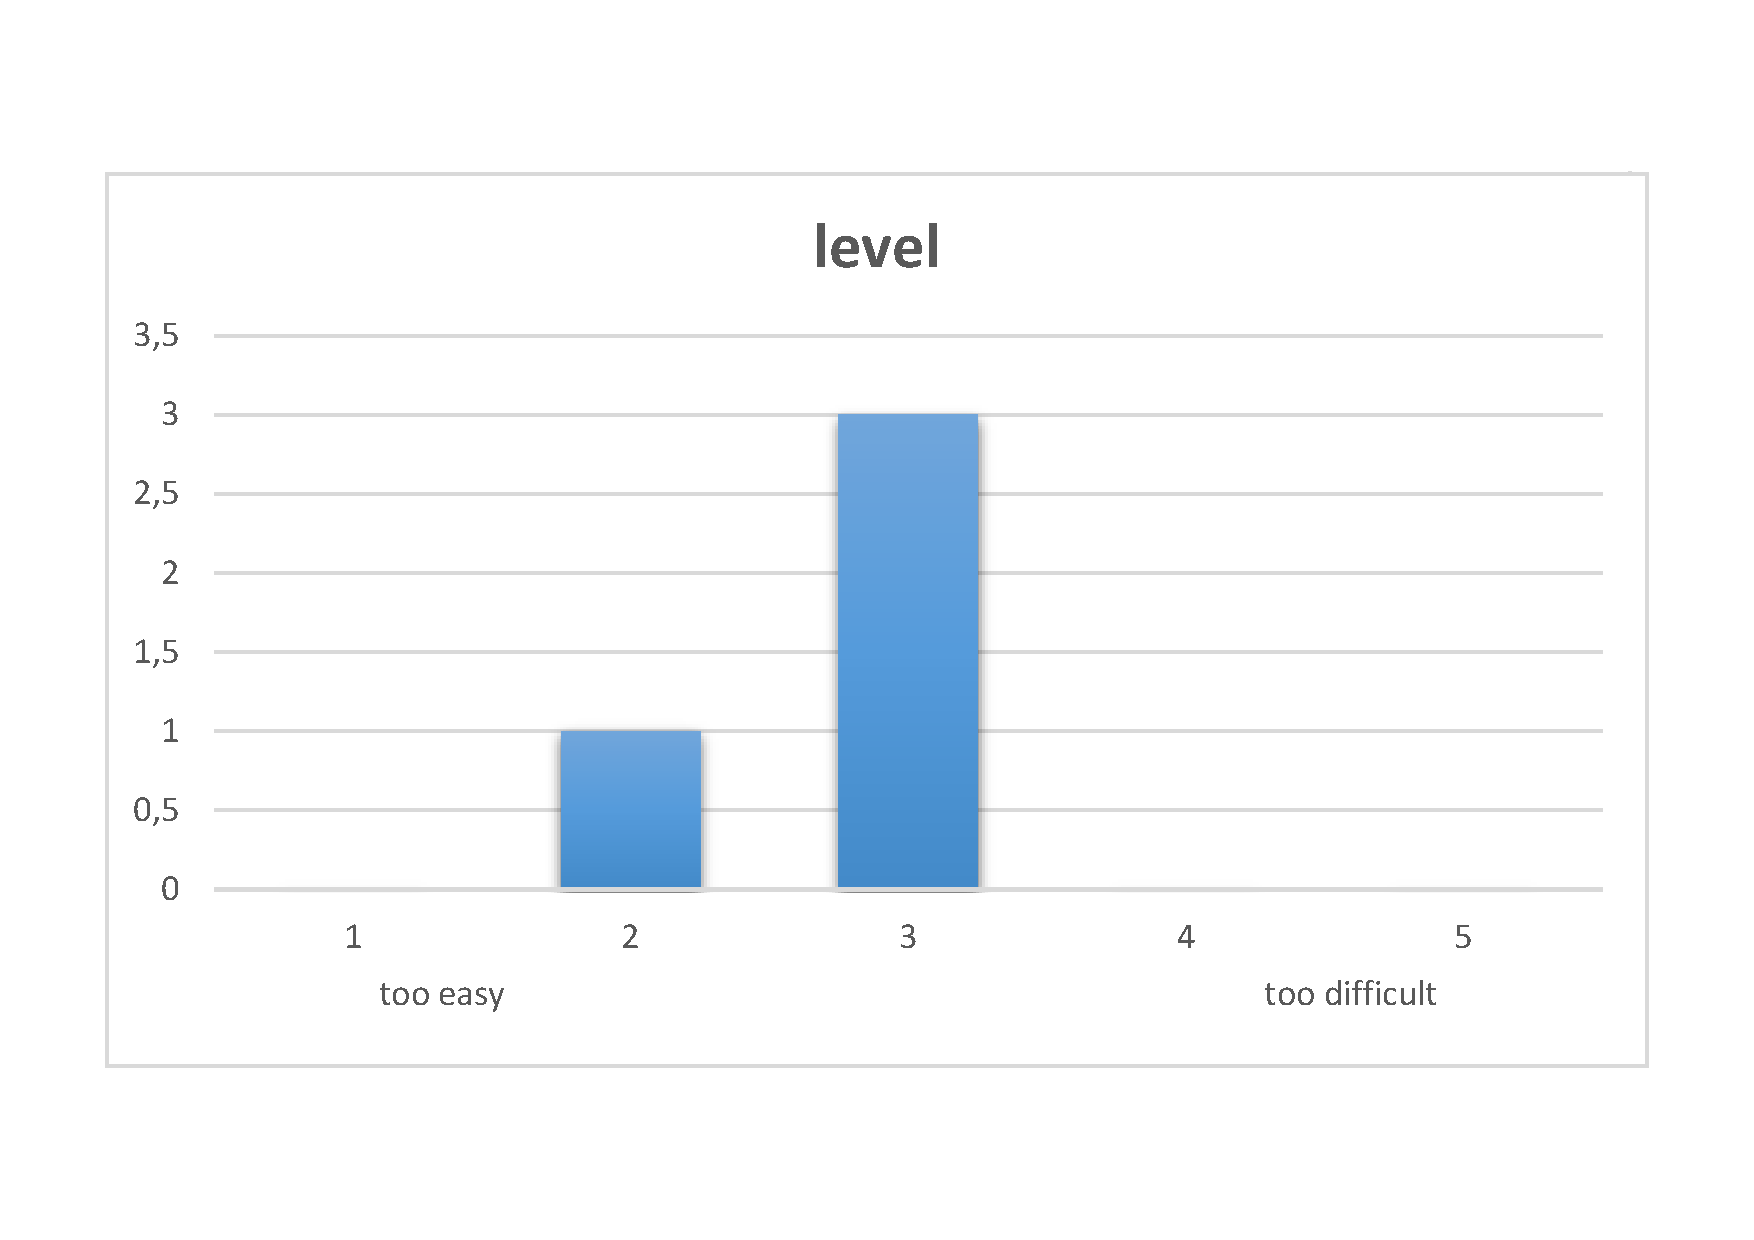
\includegraphics[width=0.5\textwidth]{eval/anders/level.pdf}}
\hfill %
\subfloat[\label{b}]{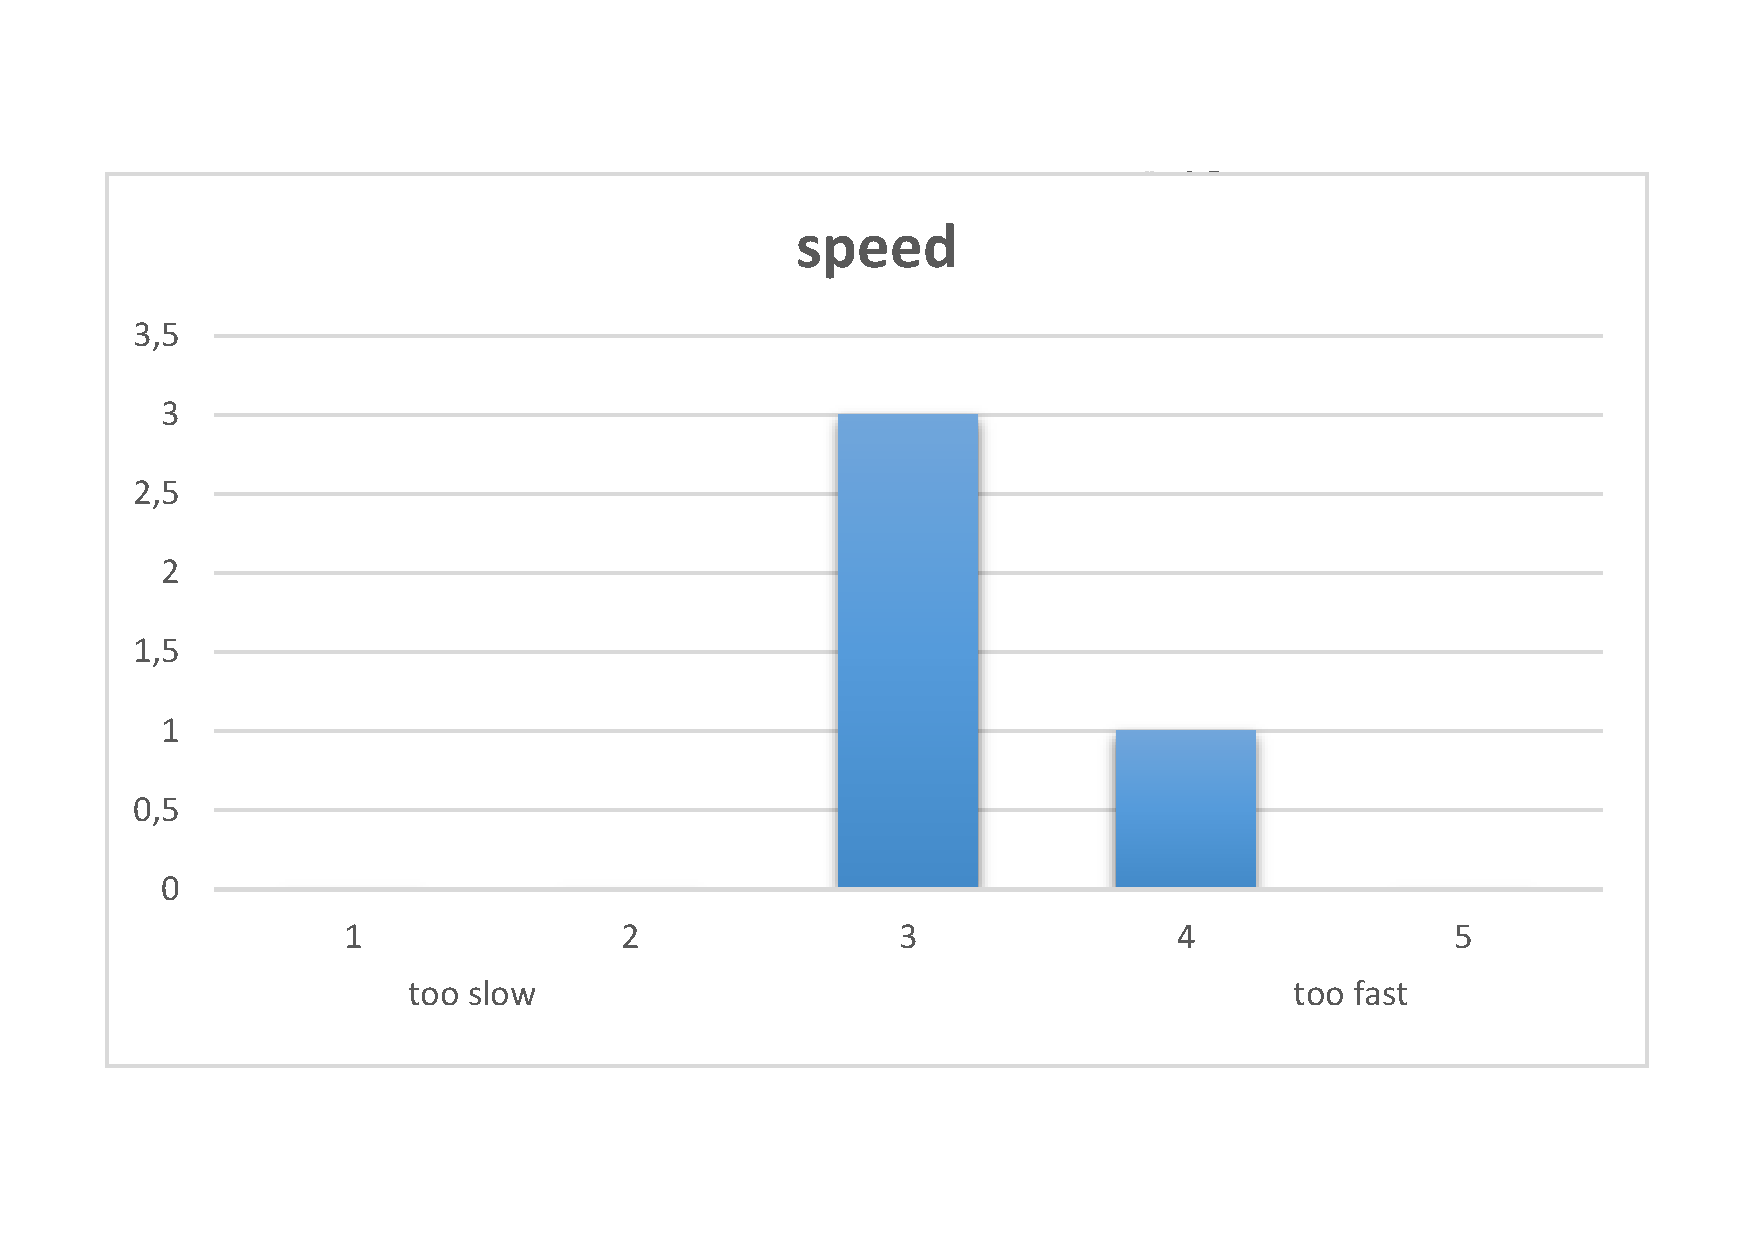
\includegraphics[width=0.5\textwidth]{eval/anders/speed.pdf}}
\hfill\null % 
\caption{Lecture: C. F. Anders  - "Jets to the future: Boosted boson and top jets as a probe for new physics"}
\end{figure} 

\subsubsection{Lecture: N. Berger - "Two, three, many? How quarks make hadrons"}

\begin{figure}[H]
\centering
\null\hfill %
\subfloat[\label{b}]{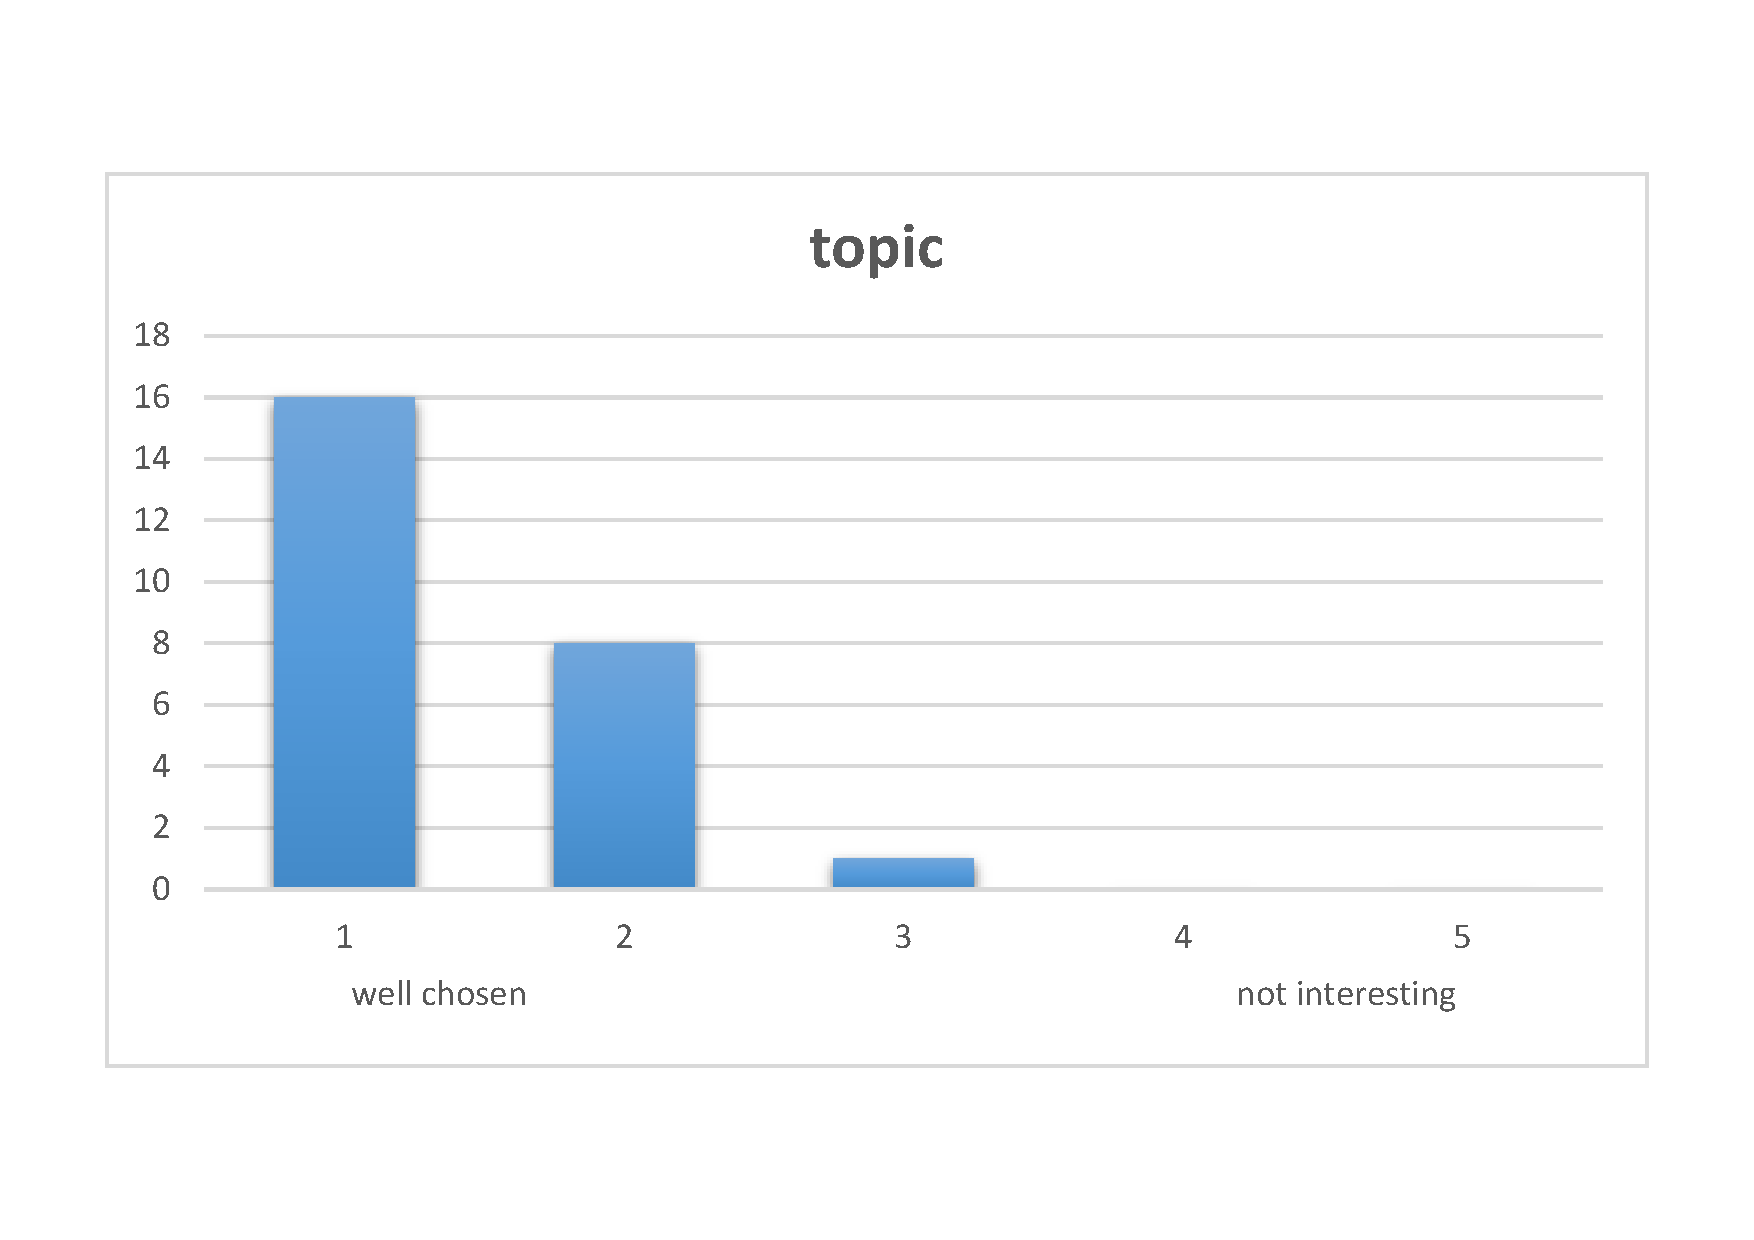
\includegraphics[width=0.5\textwidth]{eval/berger/topic.pdf}}
\hfill %
\subfloat[\label{b}]{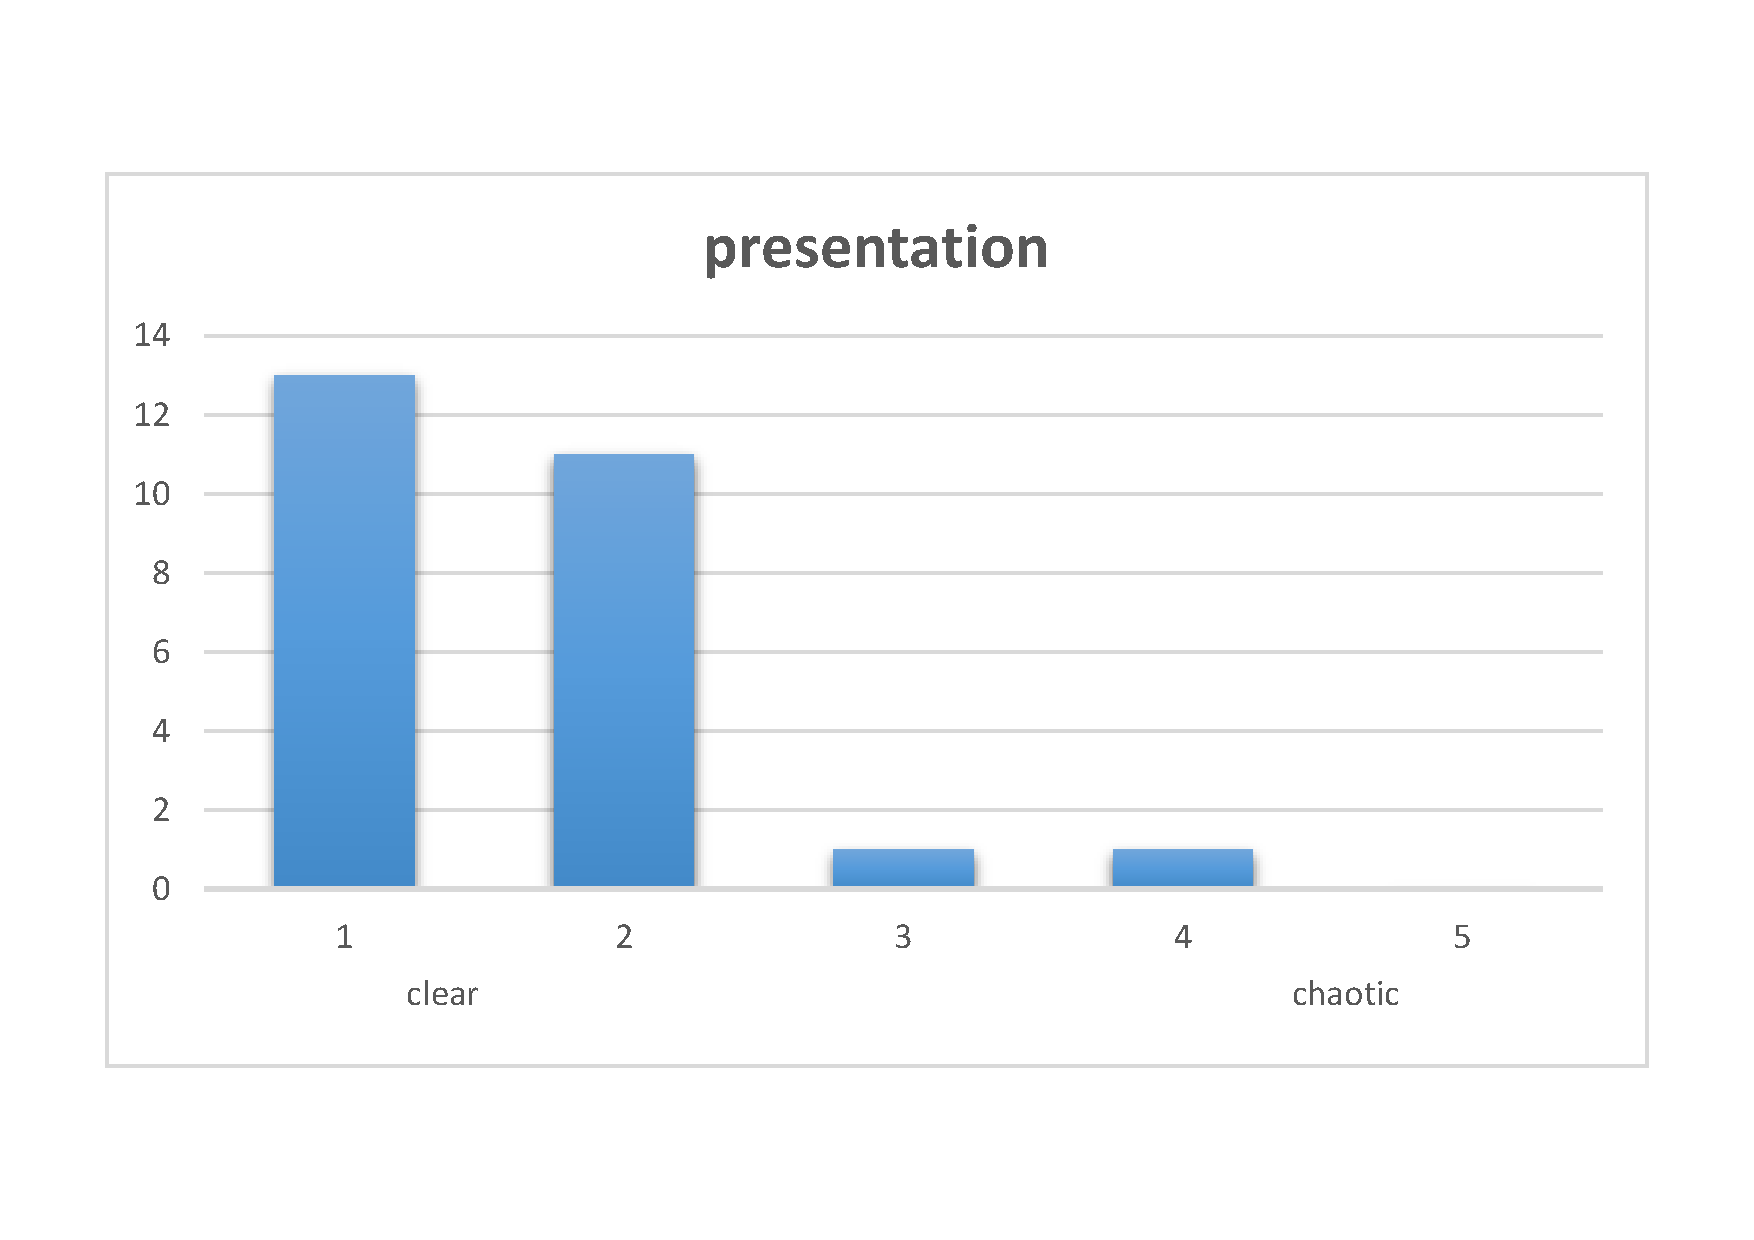
\includegraphics[width=0.5\textwidth]{eval/berger/presentation.pdf}}
\hfill %
\subfloat[\label{b}]{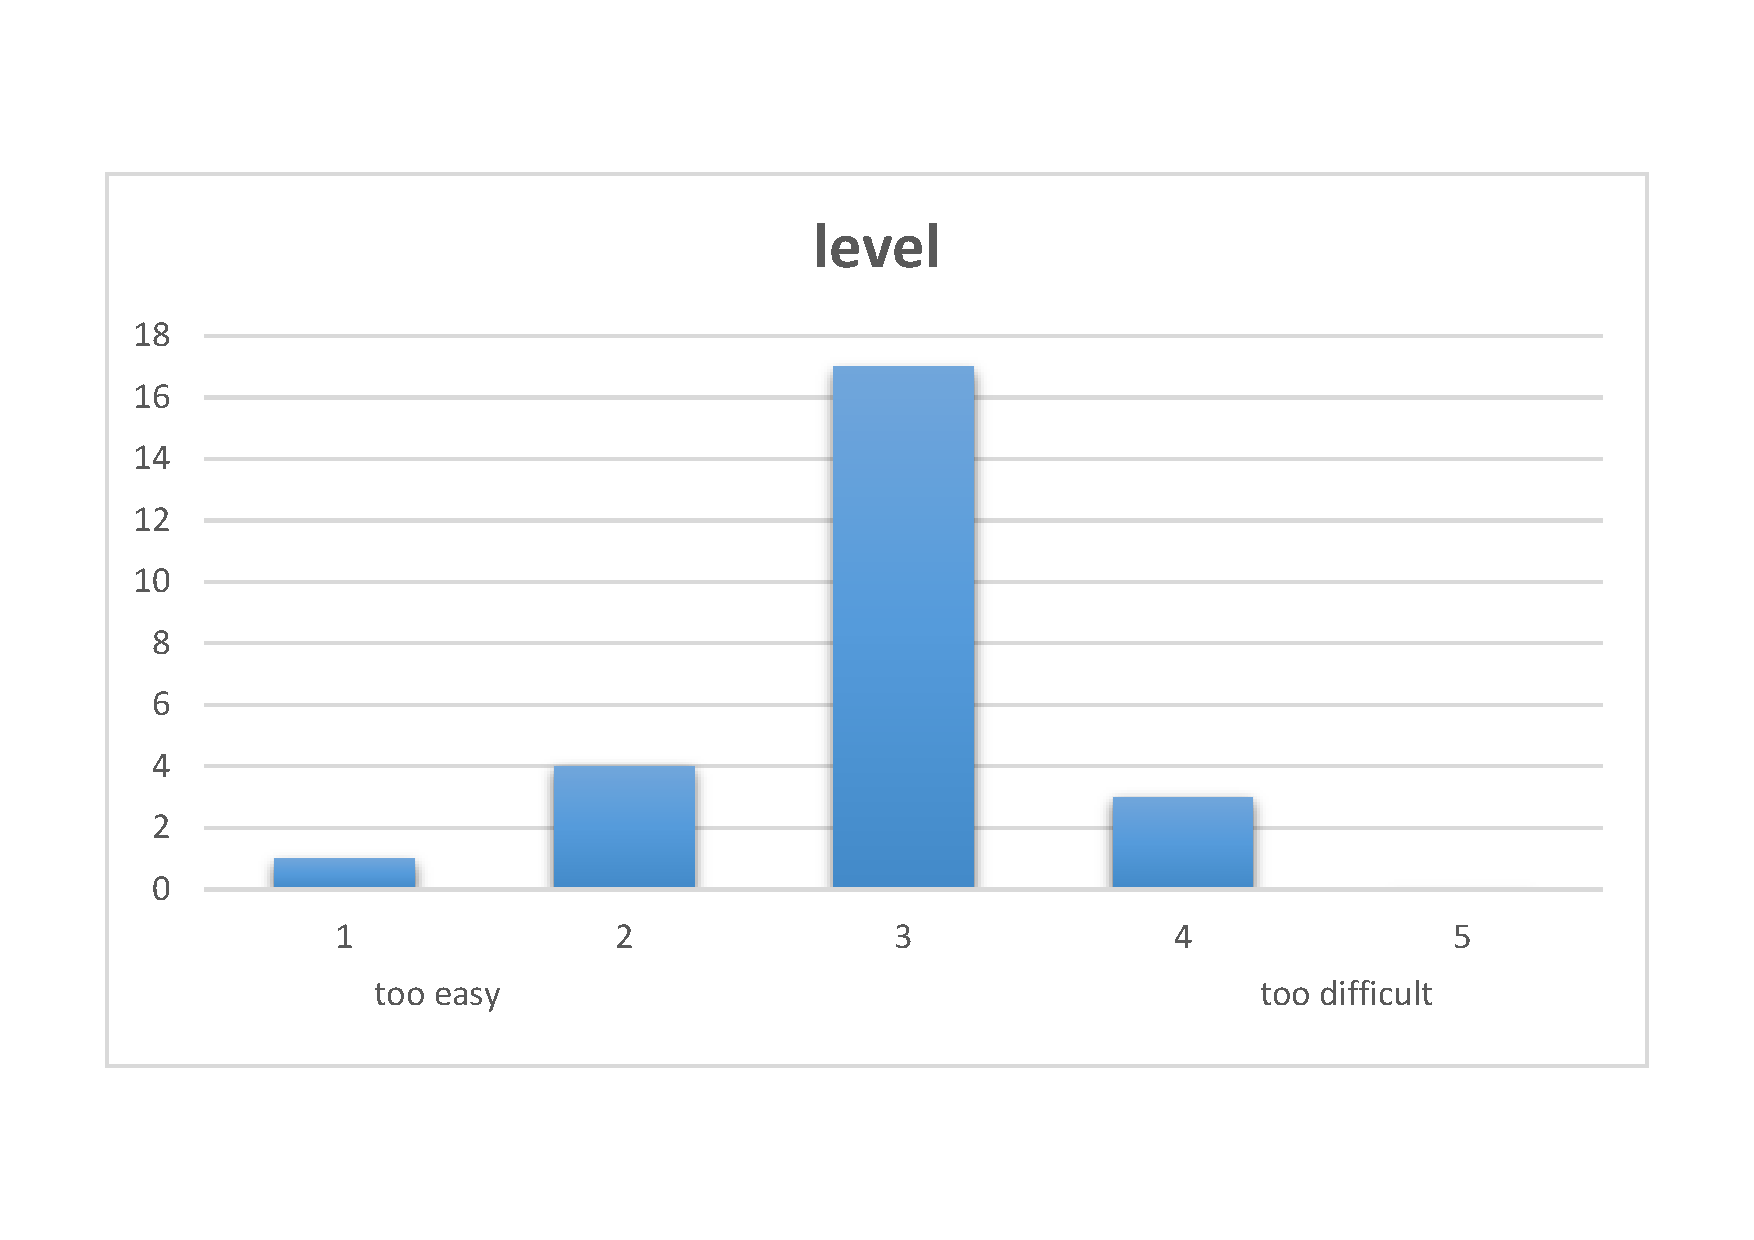
\includegraphics[width=0.5\textwidth]{eval/berger/level.pdf}}
\hfill %
\subfloat[\label{b}]{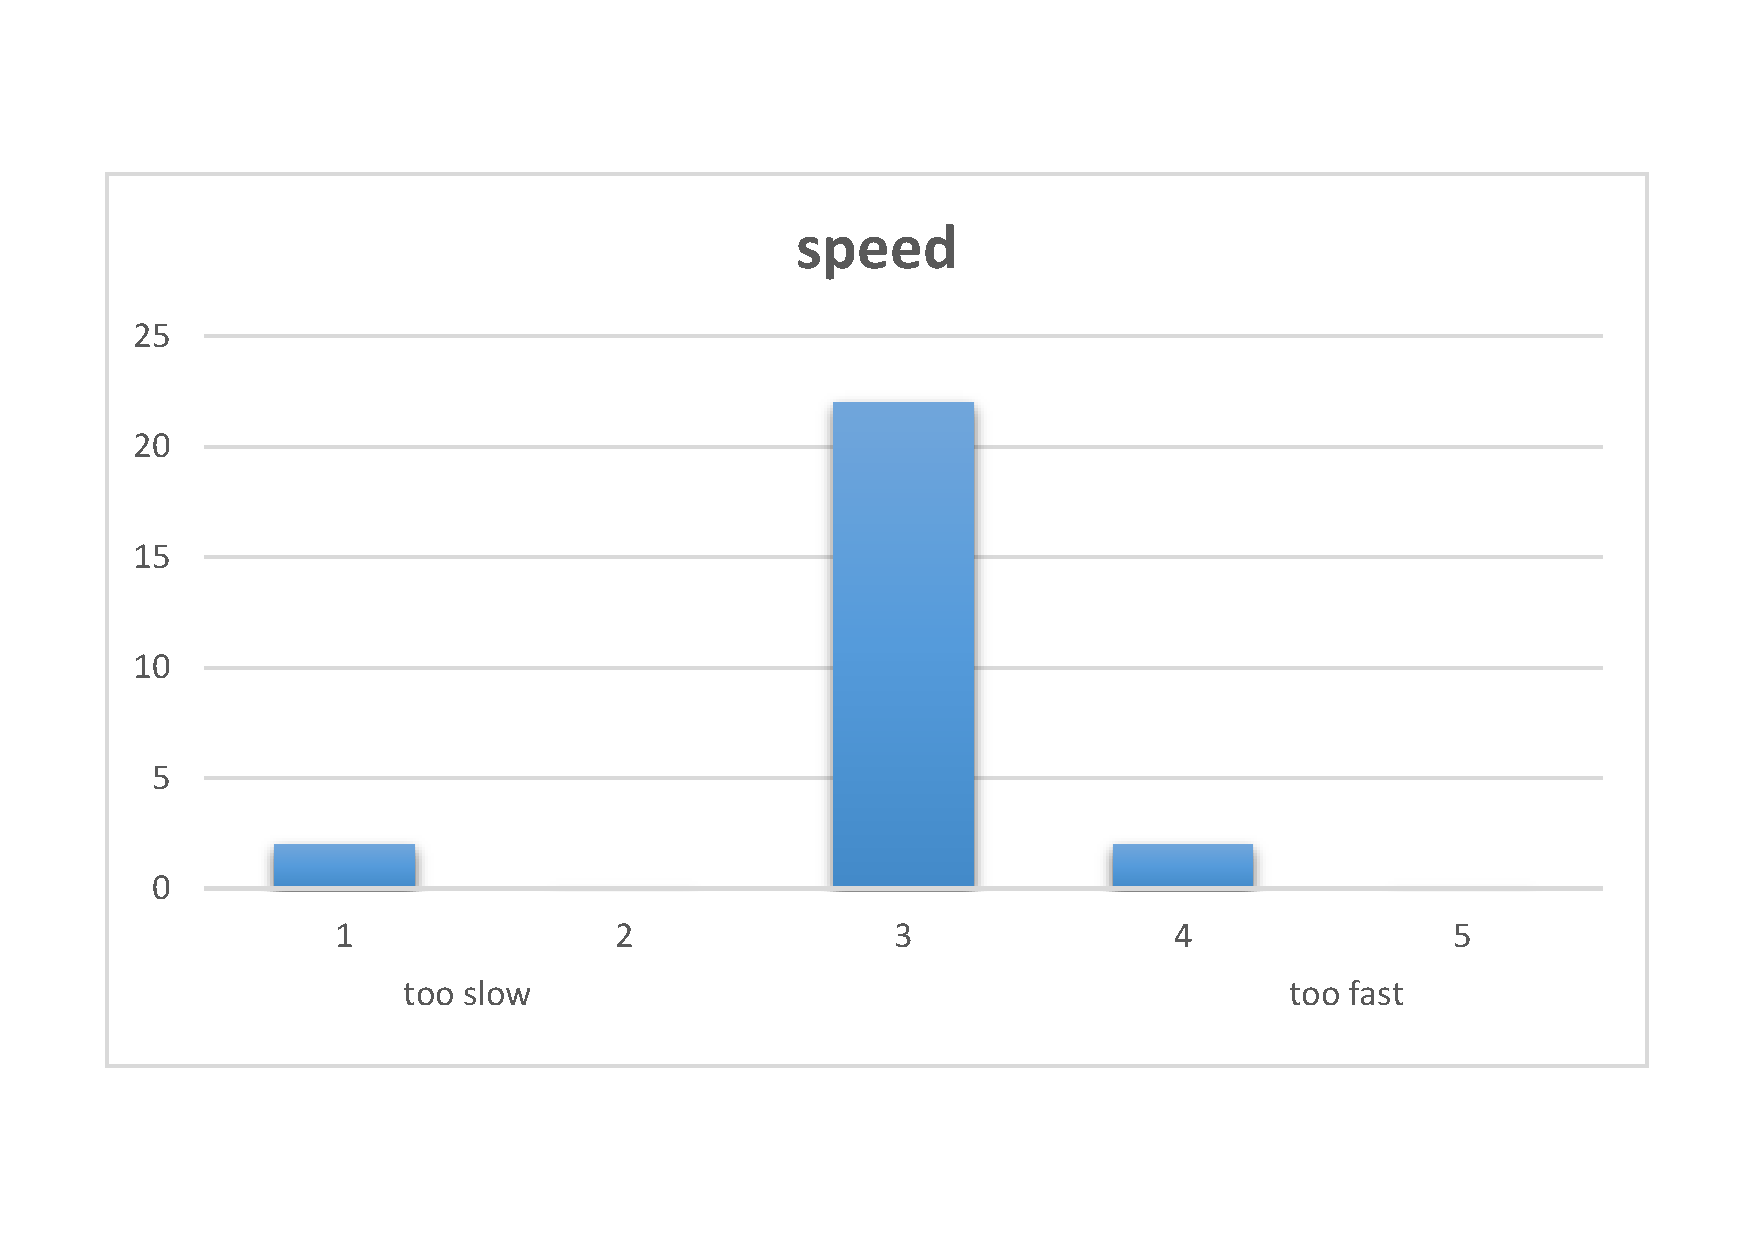
\includegraphics[width=0.5\textwidth]{eval/berger/speed.pdf}}
\hfill\null % 
\caption{Lecture: N. Berger - "Two, three, many? How quarks make hadrons"}
\end{figure} 

\subsubsection{Lecture: K. Gru{\ss}mayer - "Single-Molecule Fluorescence and Super-Resolution Imaging"}

\begin{figure}[H]
\centering
\null\hfill %
\subfloat[\label{b}]{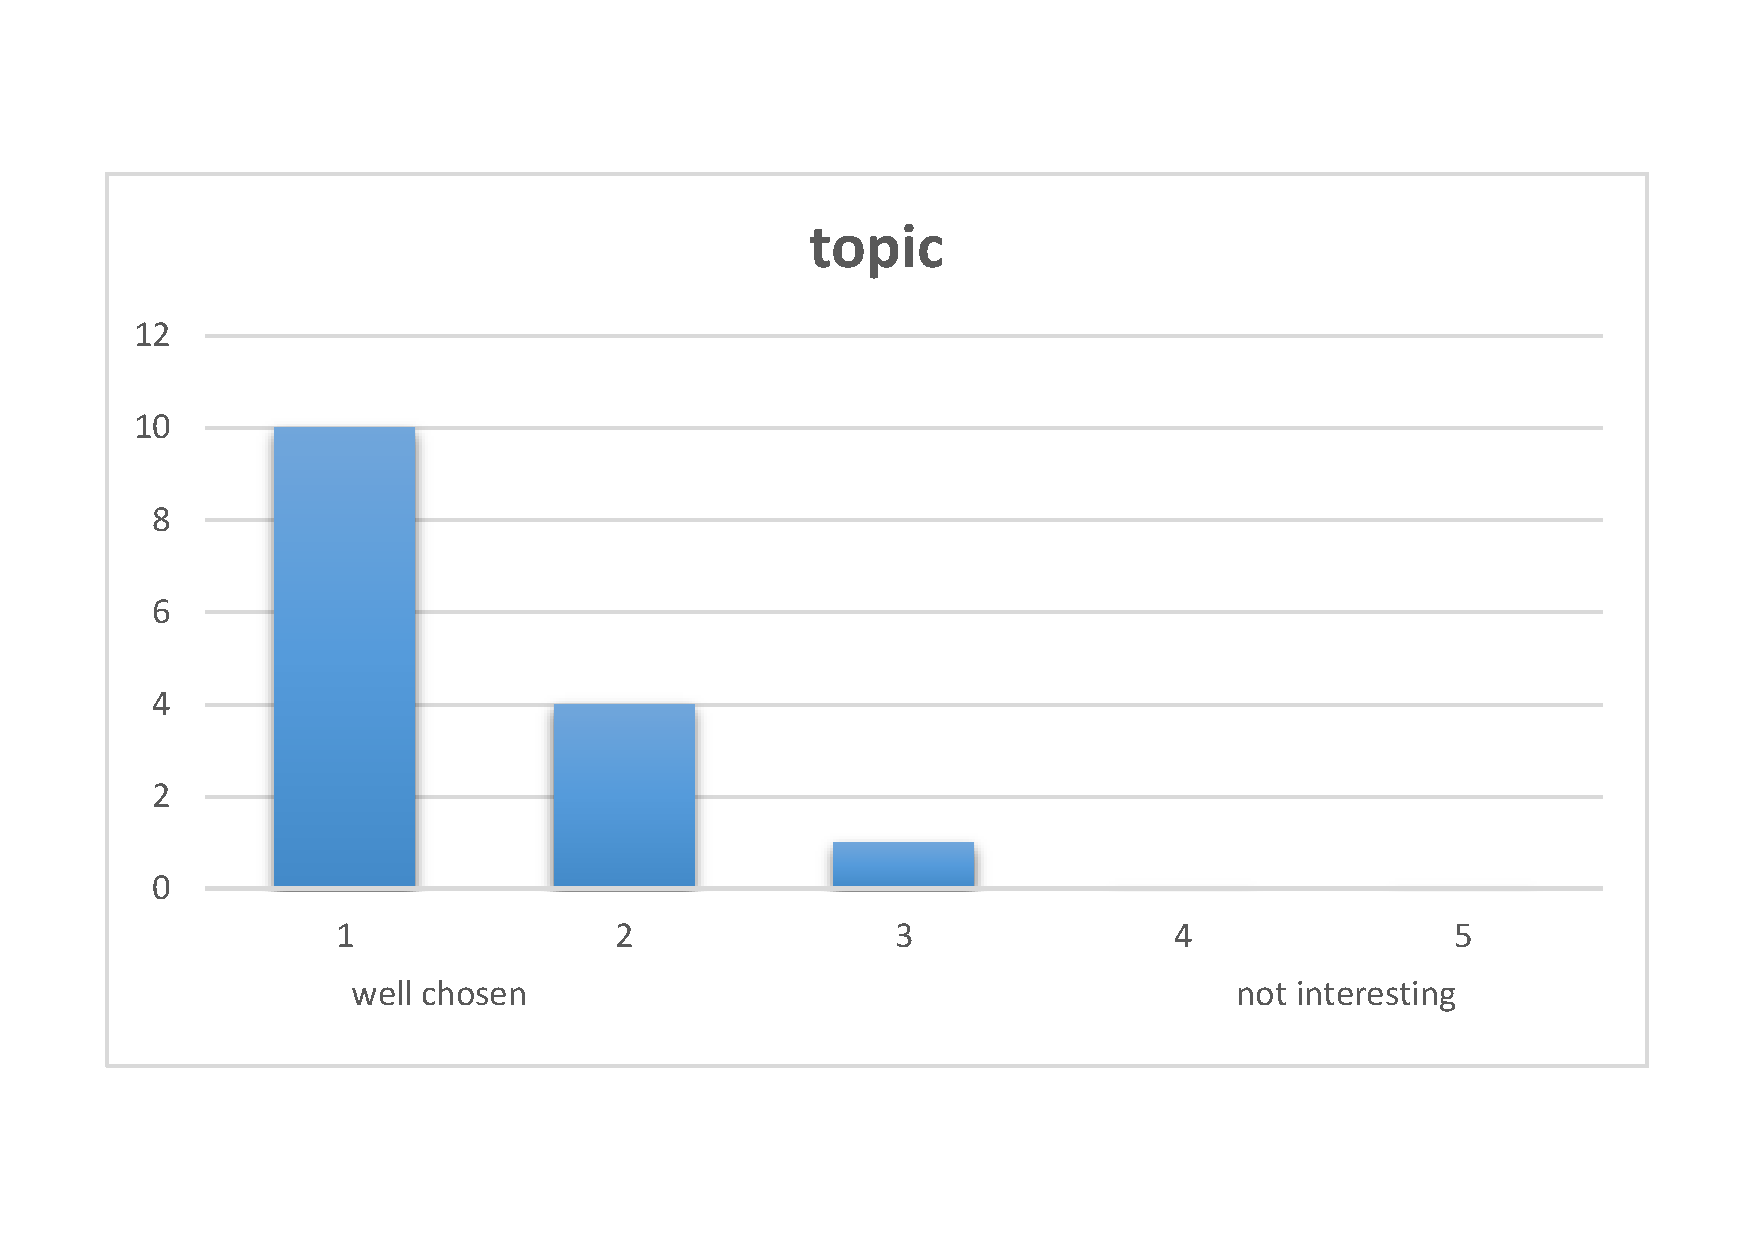
\includegraphics[width=0.5\textwidth]{eval/grussmayer/topic.pdf}}
\hfill %
\subfloat[\label{b}]{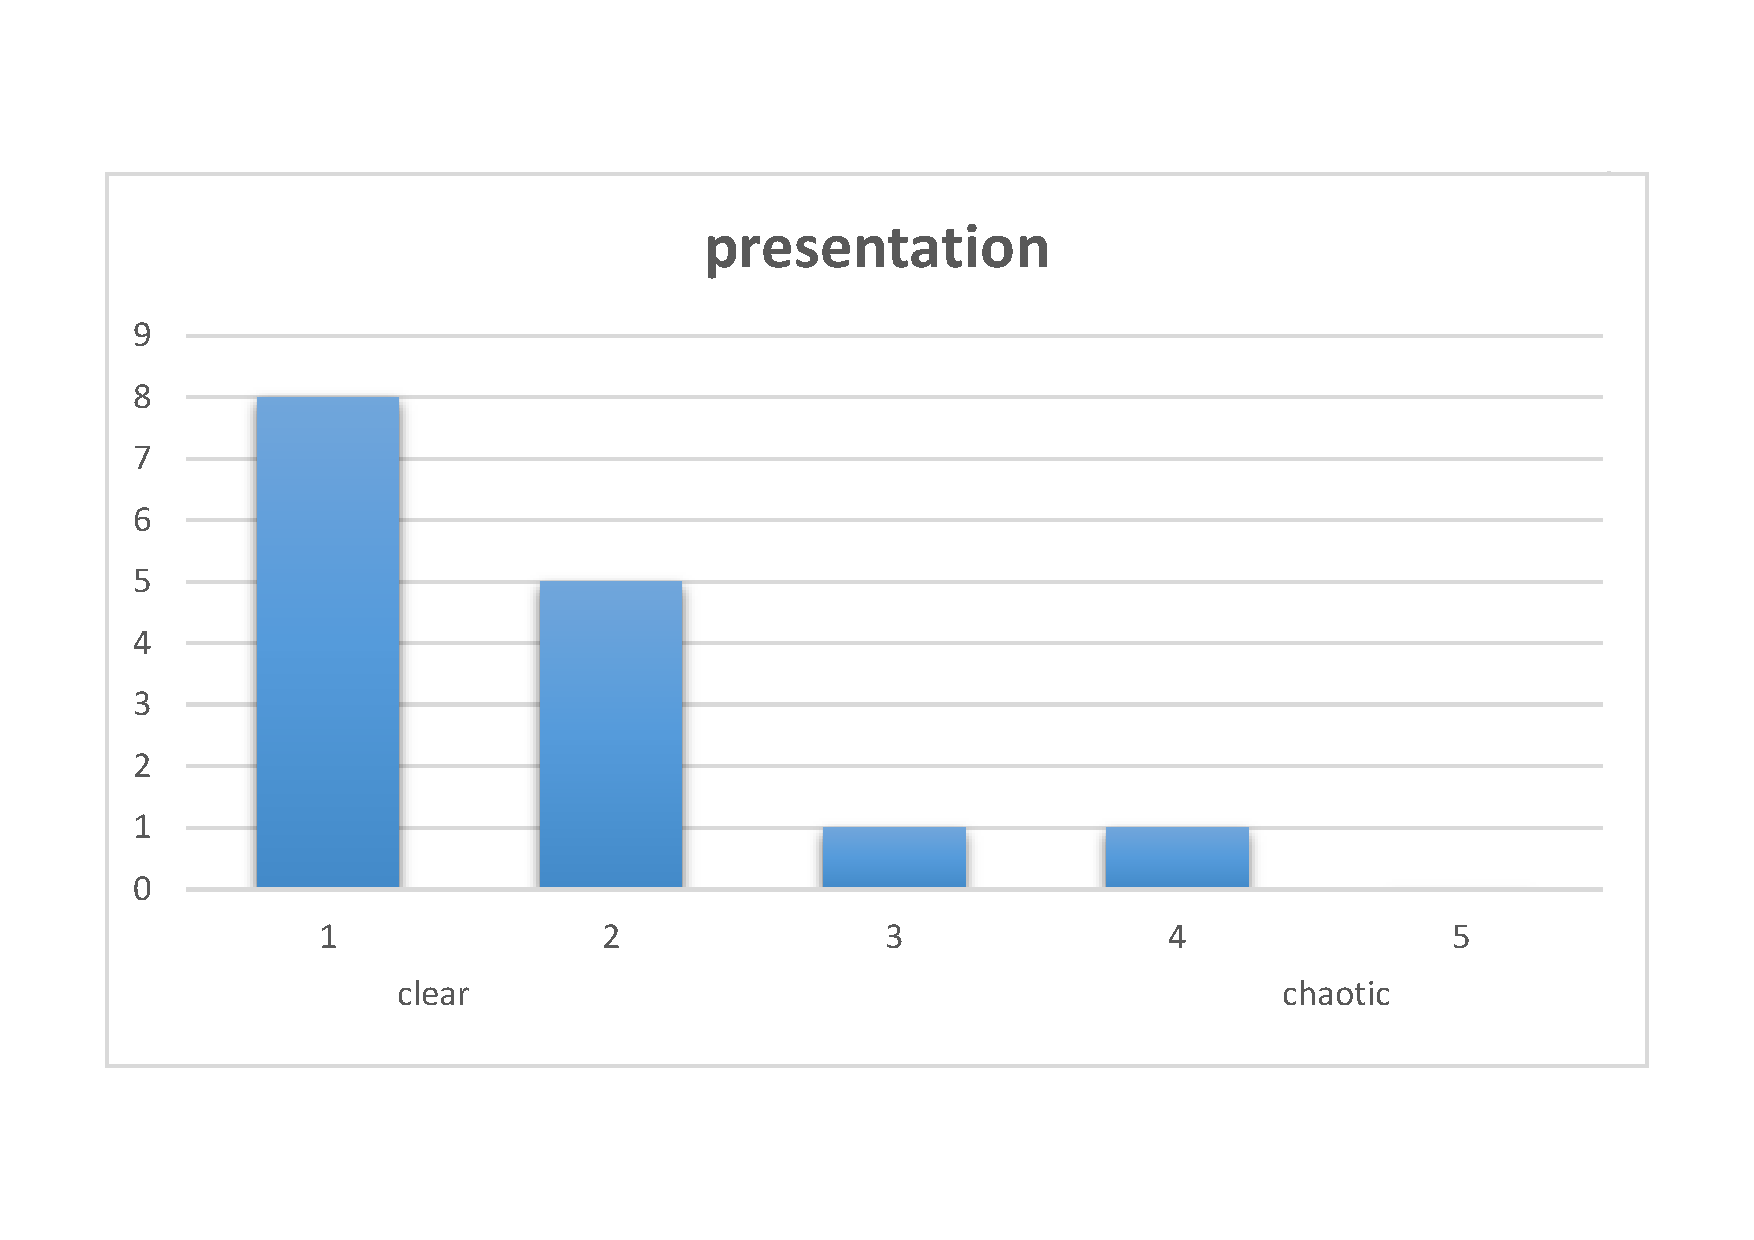
\includegraphics[width=0.5\textwidth]{eval/grussmayer/presentation.pdf}}
\hfill %
\subfloat[\label{b}]{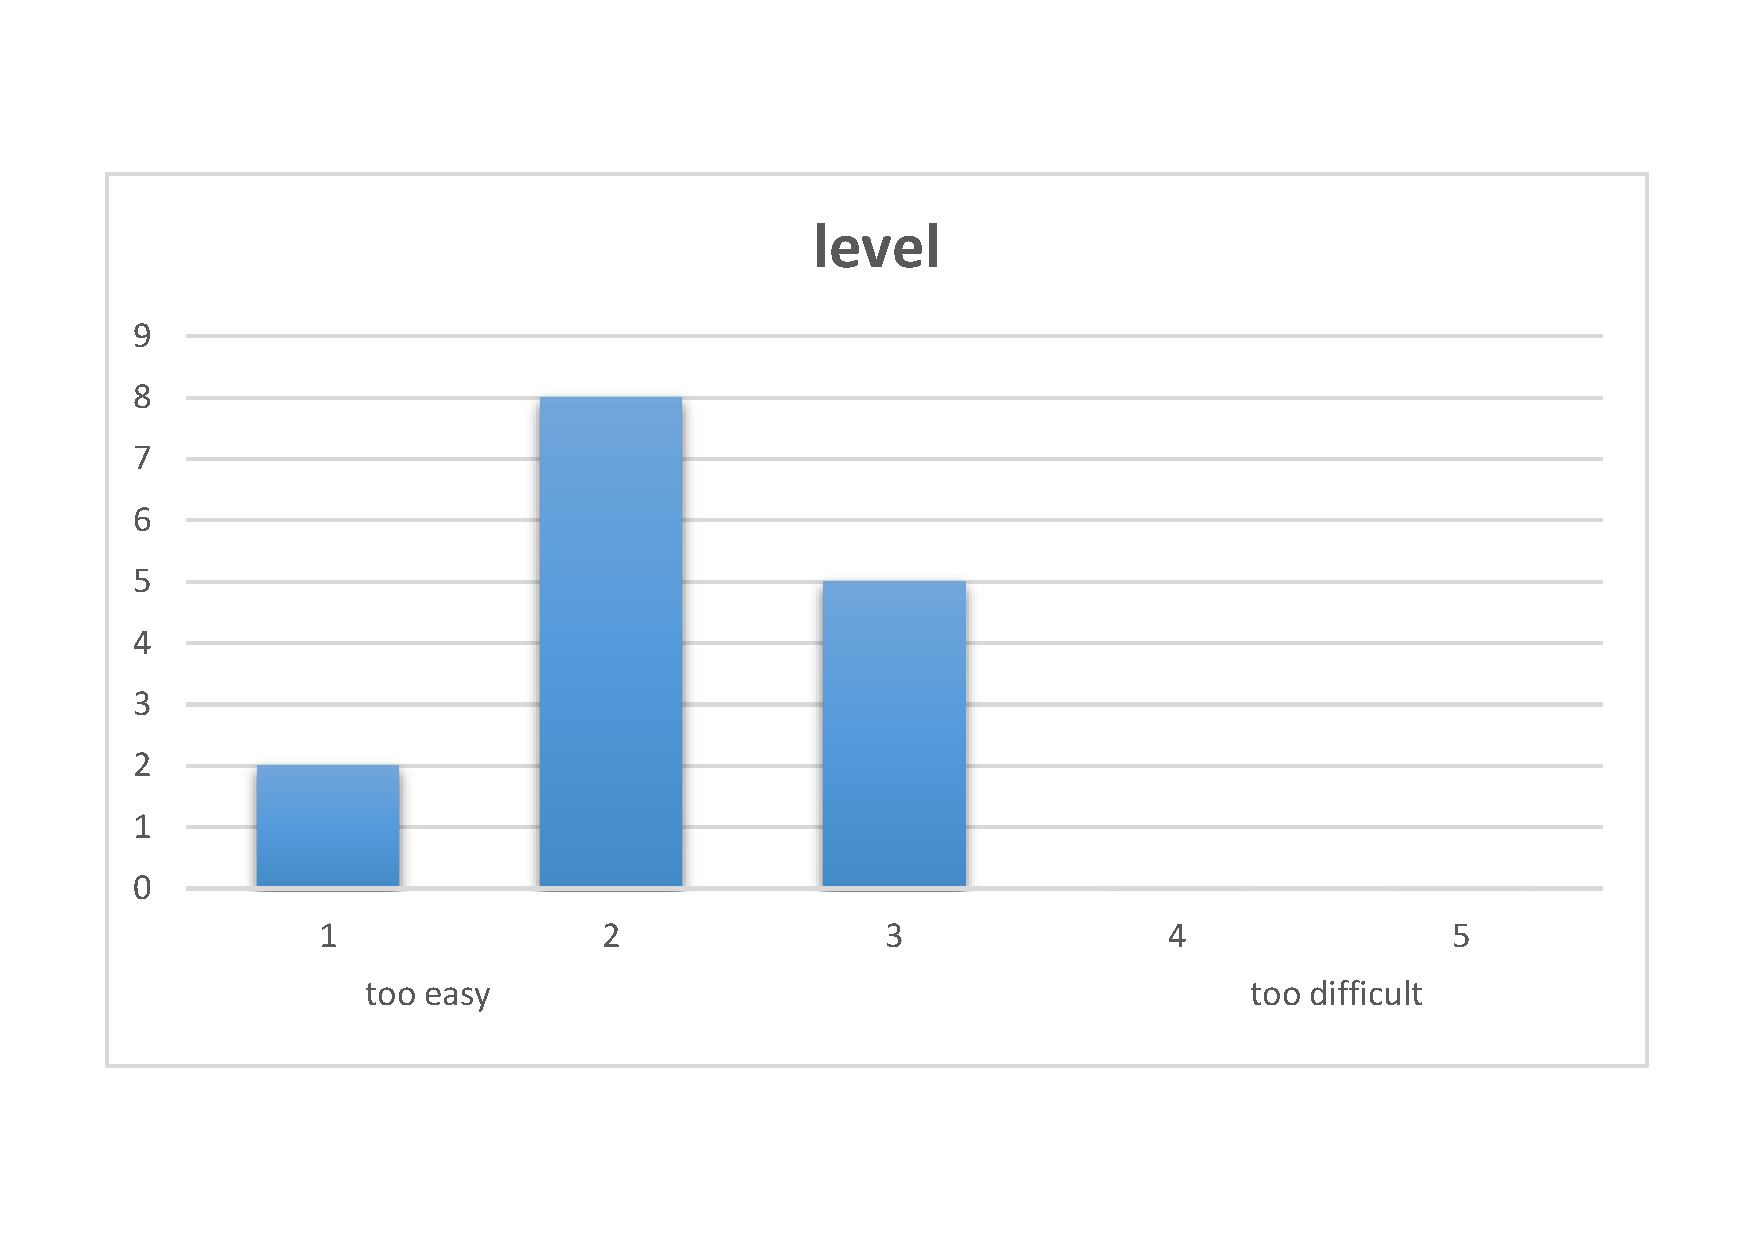
\includegraphics[width=0.5\textwidth]{eval/grussmayer/level.pdf}}
\hfill %
\subfloat[\label{b}]{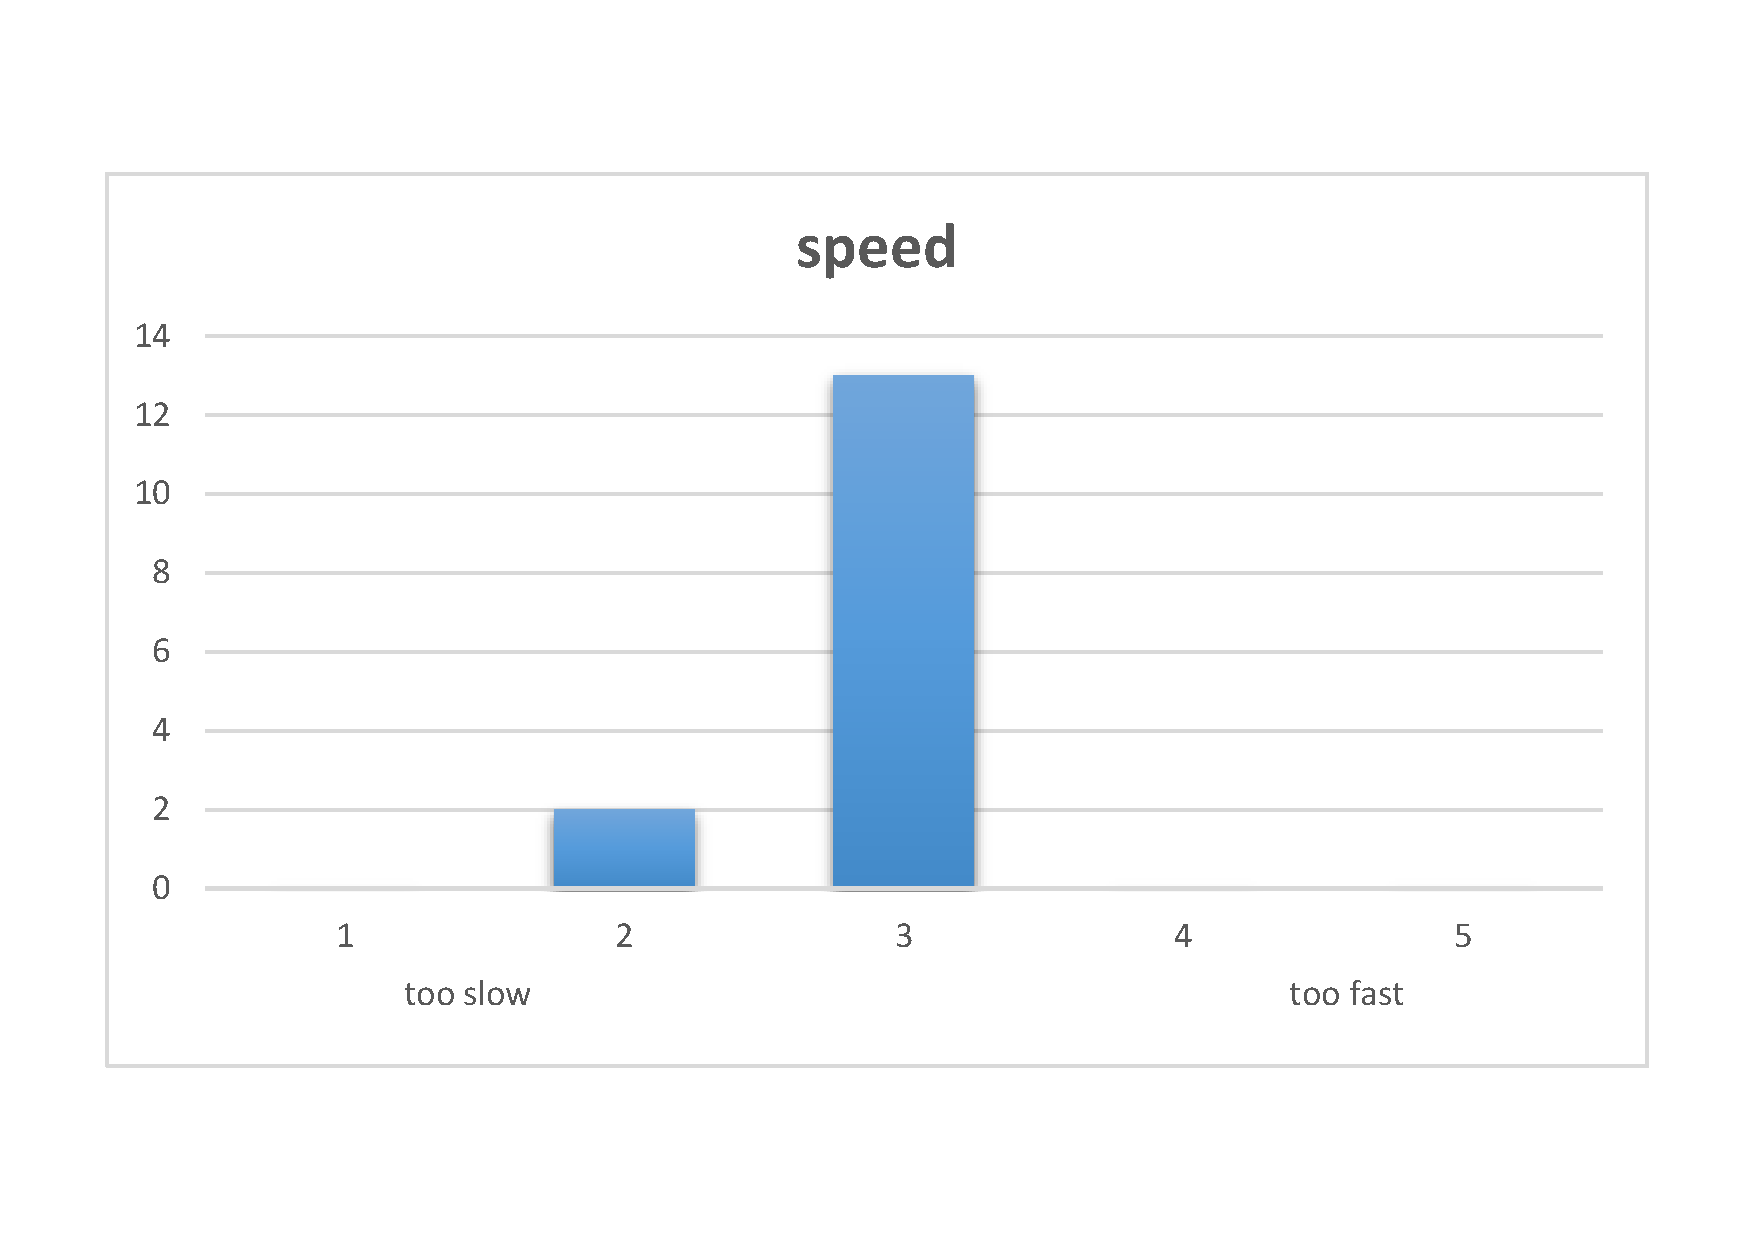
\includegraphics[width=0.5\textwidth]{eval/grussmayer/speed.pdf}}
\hfill\null % 
\caption{Lecture: K. Gru{\ss}mayer - "Single-Molecule Fluorescence and Super-Resolution Imaging"}
\end{figure}

\subsubsection{Lecture: S. Hoekstra - "Fundamental physics with cold molecules"}

\begin{figure}[H]
\centering
\null\hfill %
\subfloat[\label{b}]{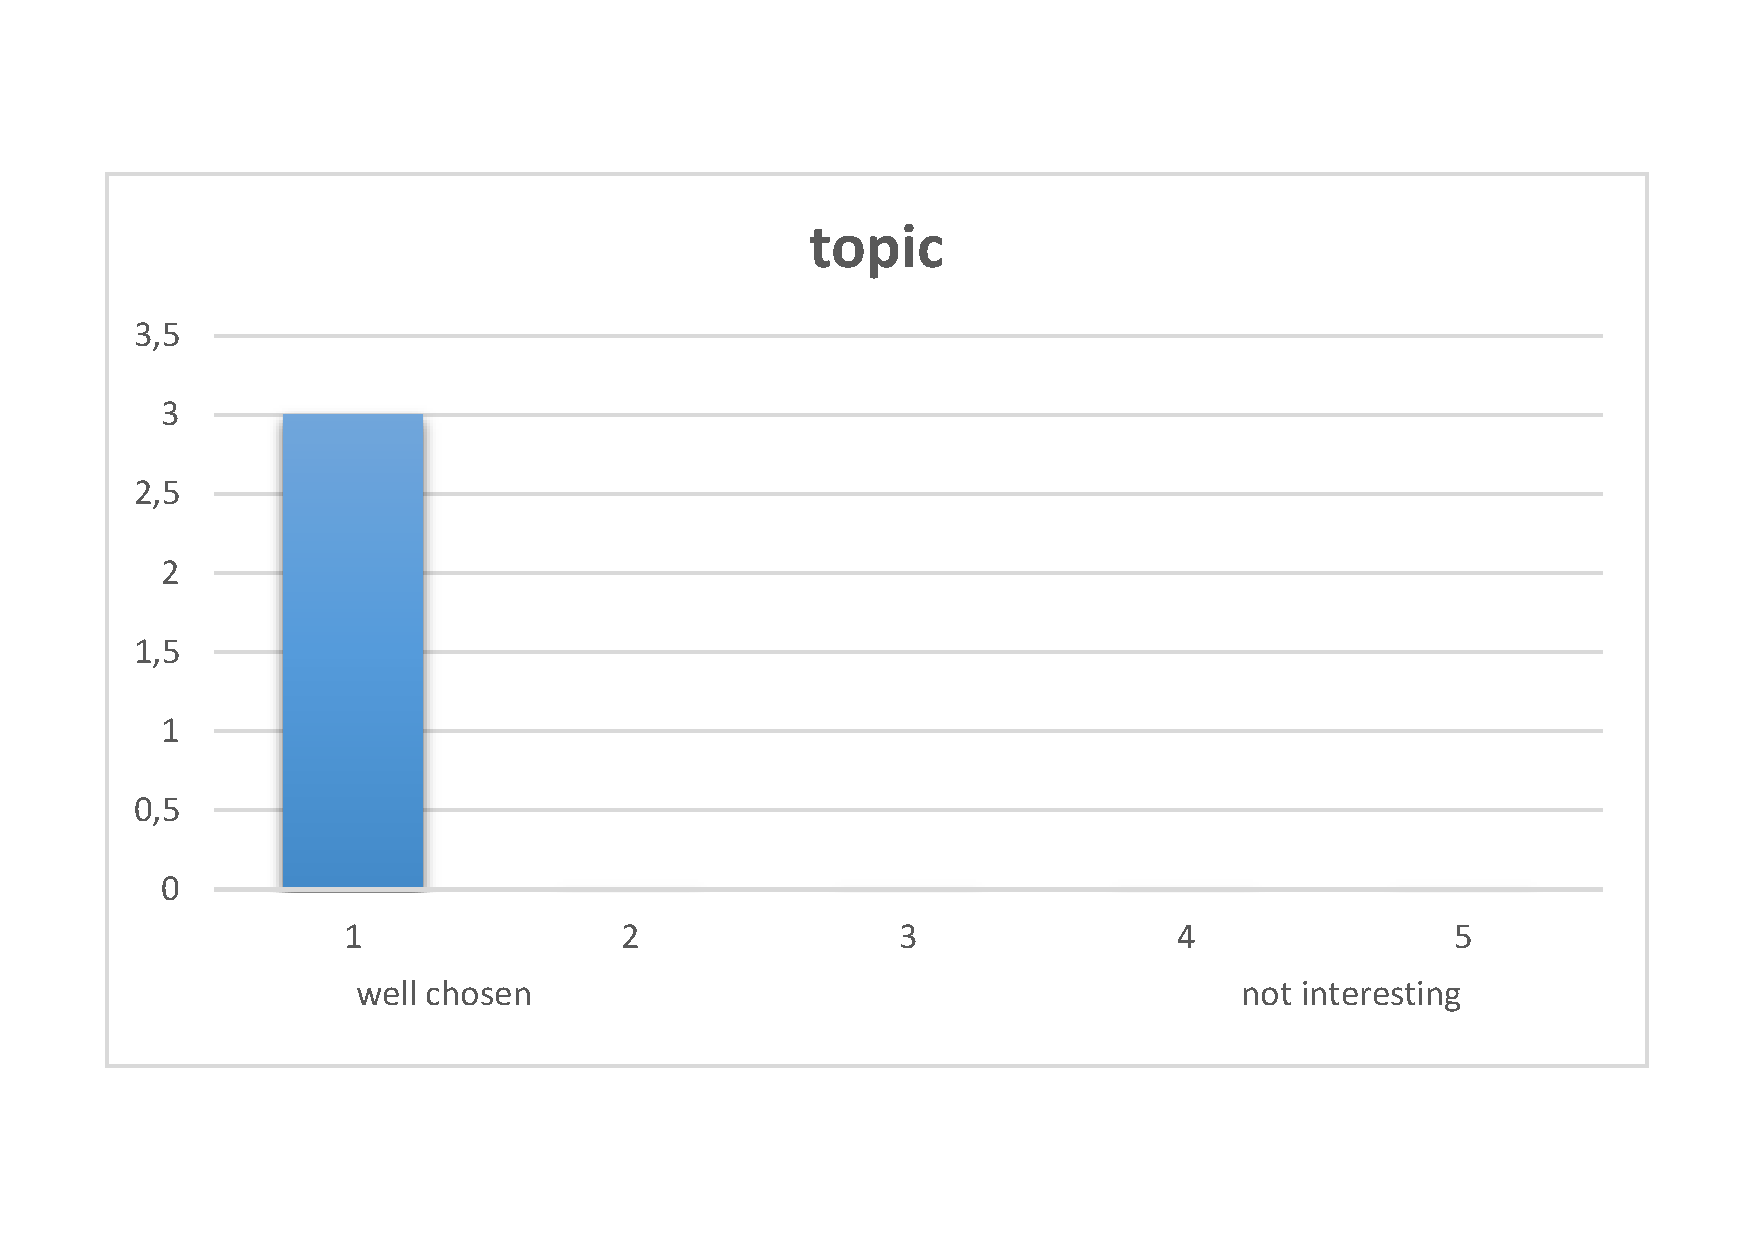
\includegraphics[width=0.5\textwidth]{eval/hoekstra/topic.pdf}}
\hfill %
\subfloat[\label{b}]{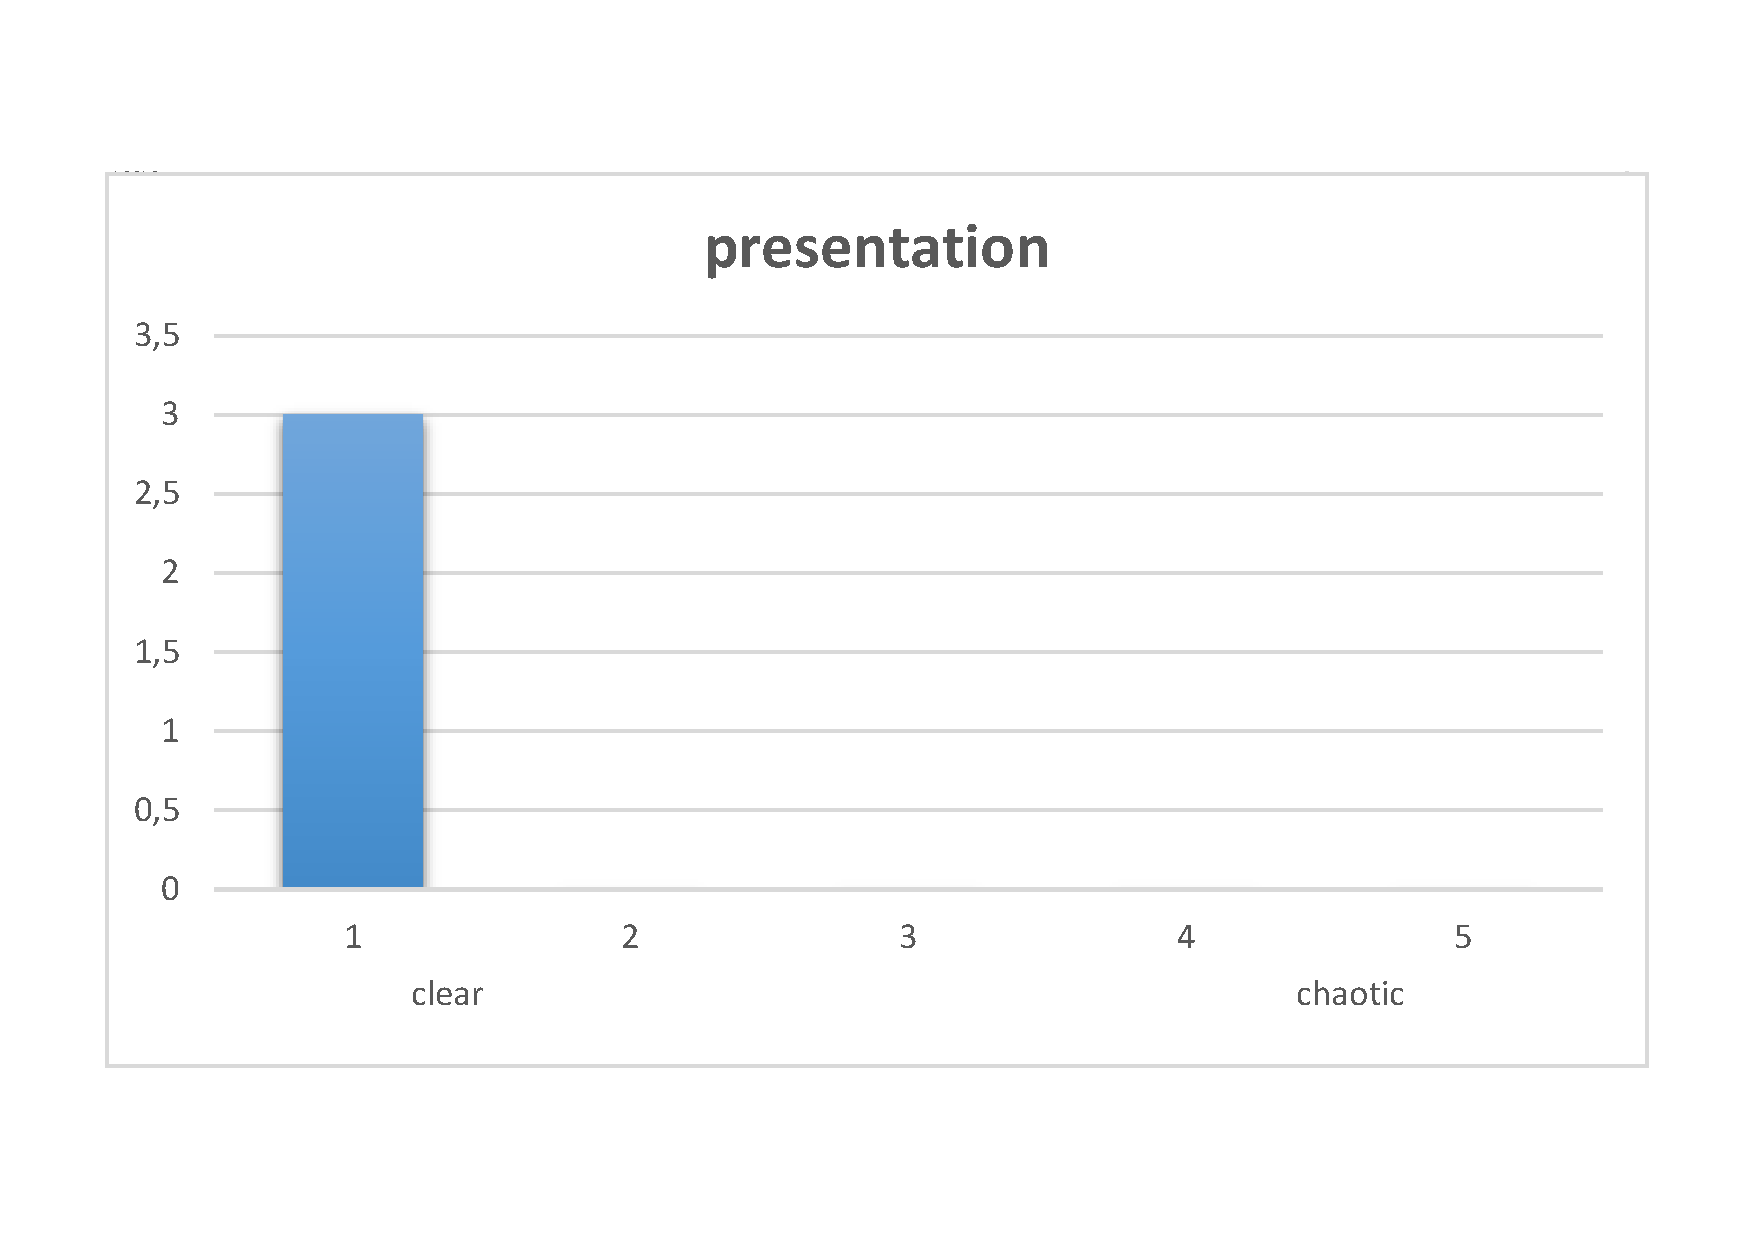
\includegraphics[width=0.5\textwidth]{eval/hoekstra/presentation.pdf}}
\hfill %
\subfloat[\label{b}]{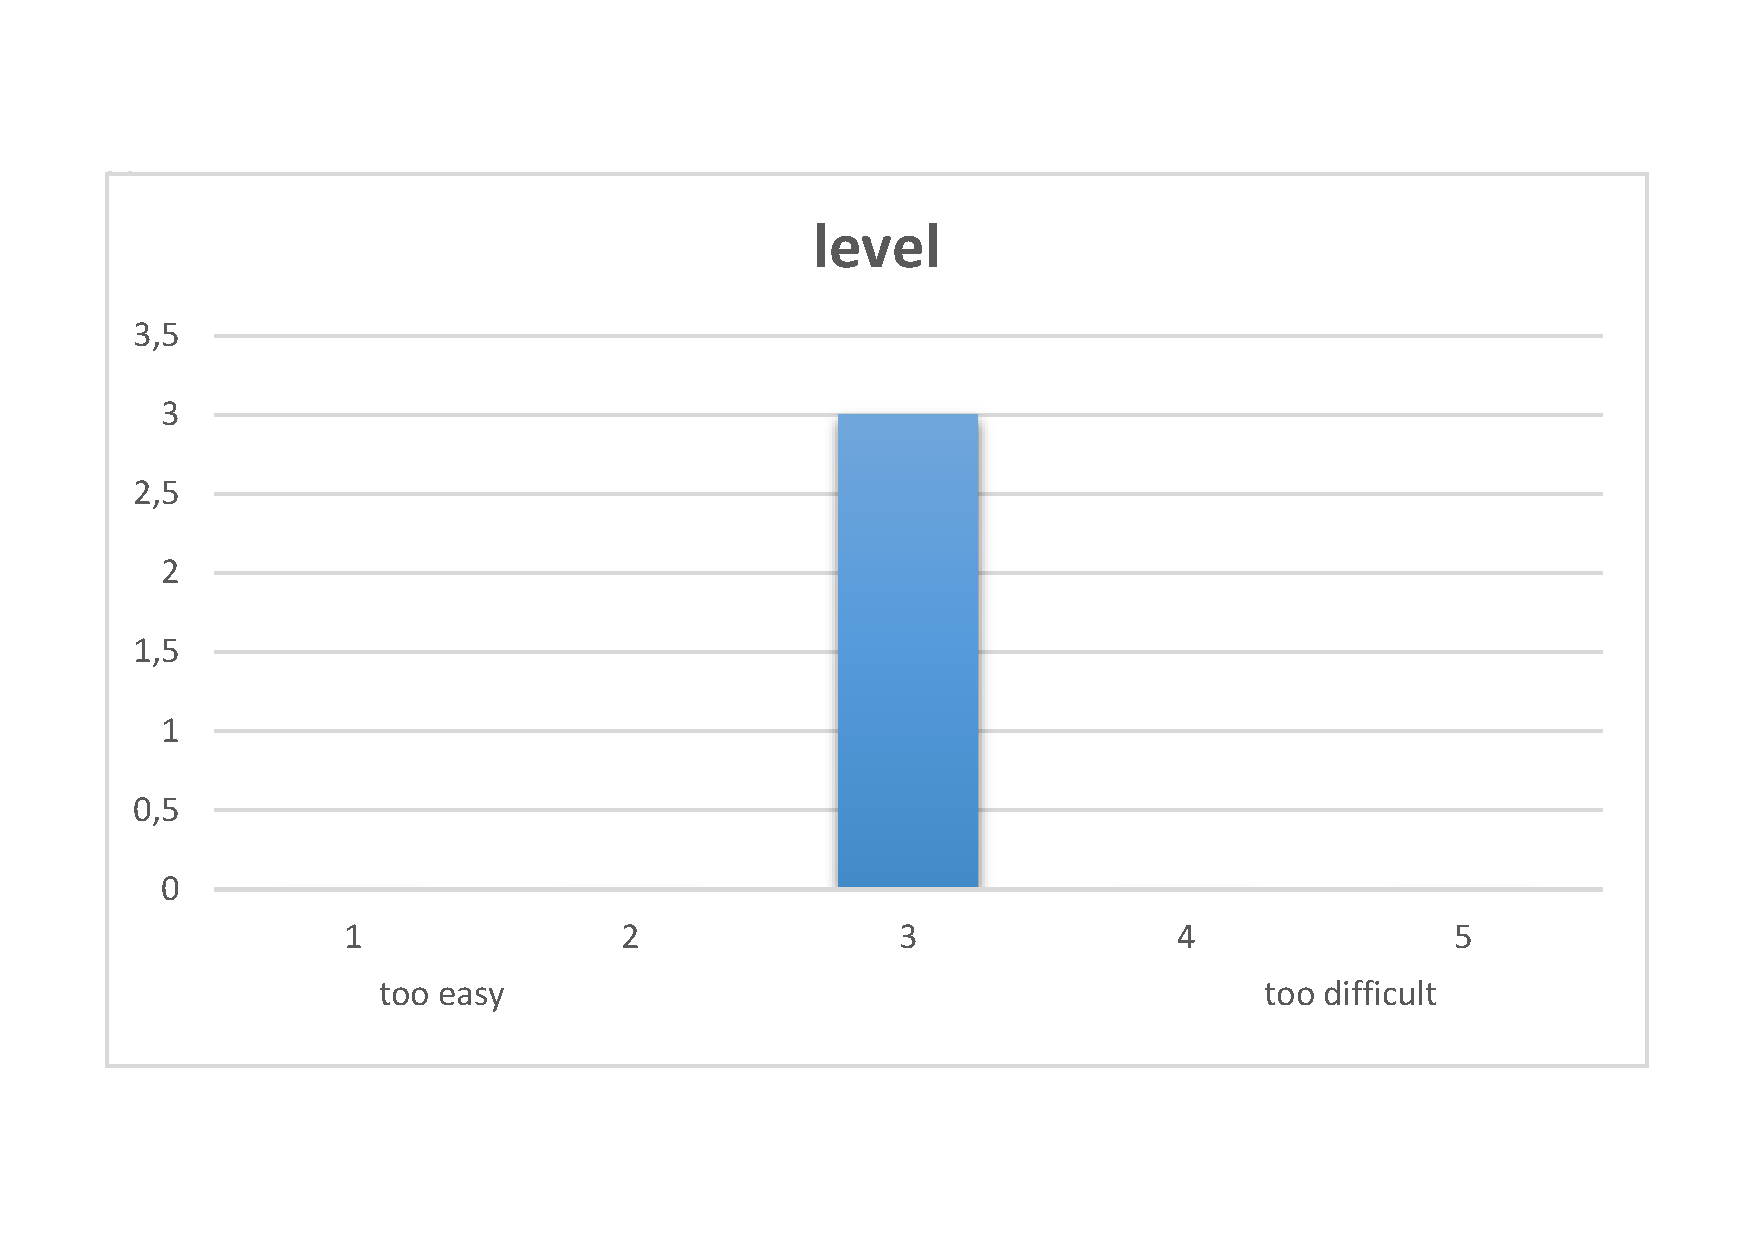
\includegraphics[width=0.5\textwidth]{eval/hoekstra/level.pdf}}
\hfill %
\subfloat[\label{b}]{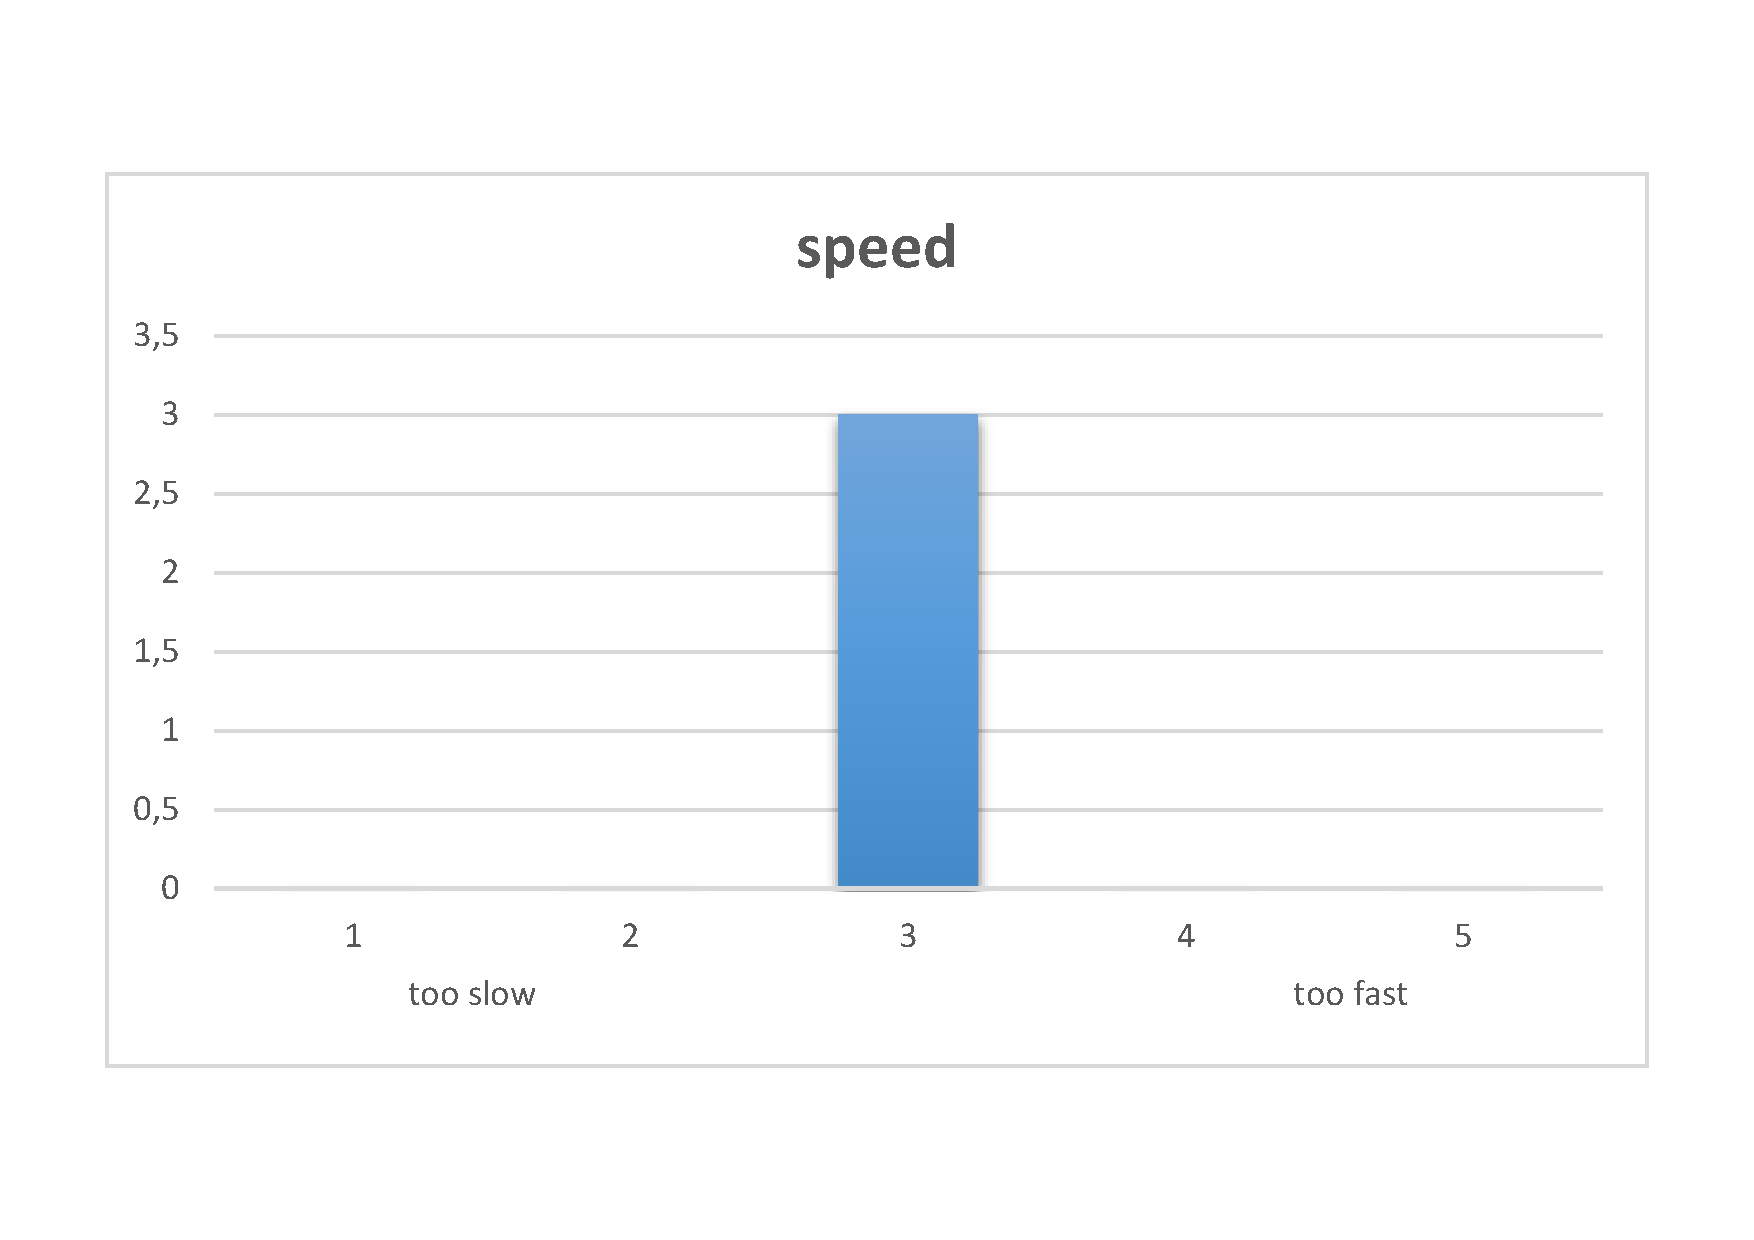
\includegraphics[width=0.5\textwidth]{eval/hoekstra/speed.pdf}}
\hfill\null % 
\caption{Lecture: S. Hoekstra - "Fundamental physics with cold molecules"}
\end{figure}


\subsubsection{Lecture: F. Jendrzejewski - "Engineering static and dynamical gauge fields with ultracold matter"}

\begin{figure}[H]
\centering
\null\hfill %
\subfloat[\label{b}]{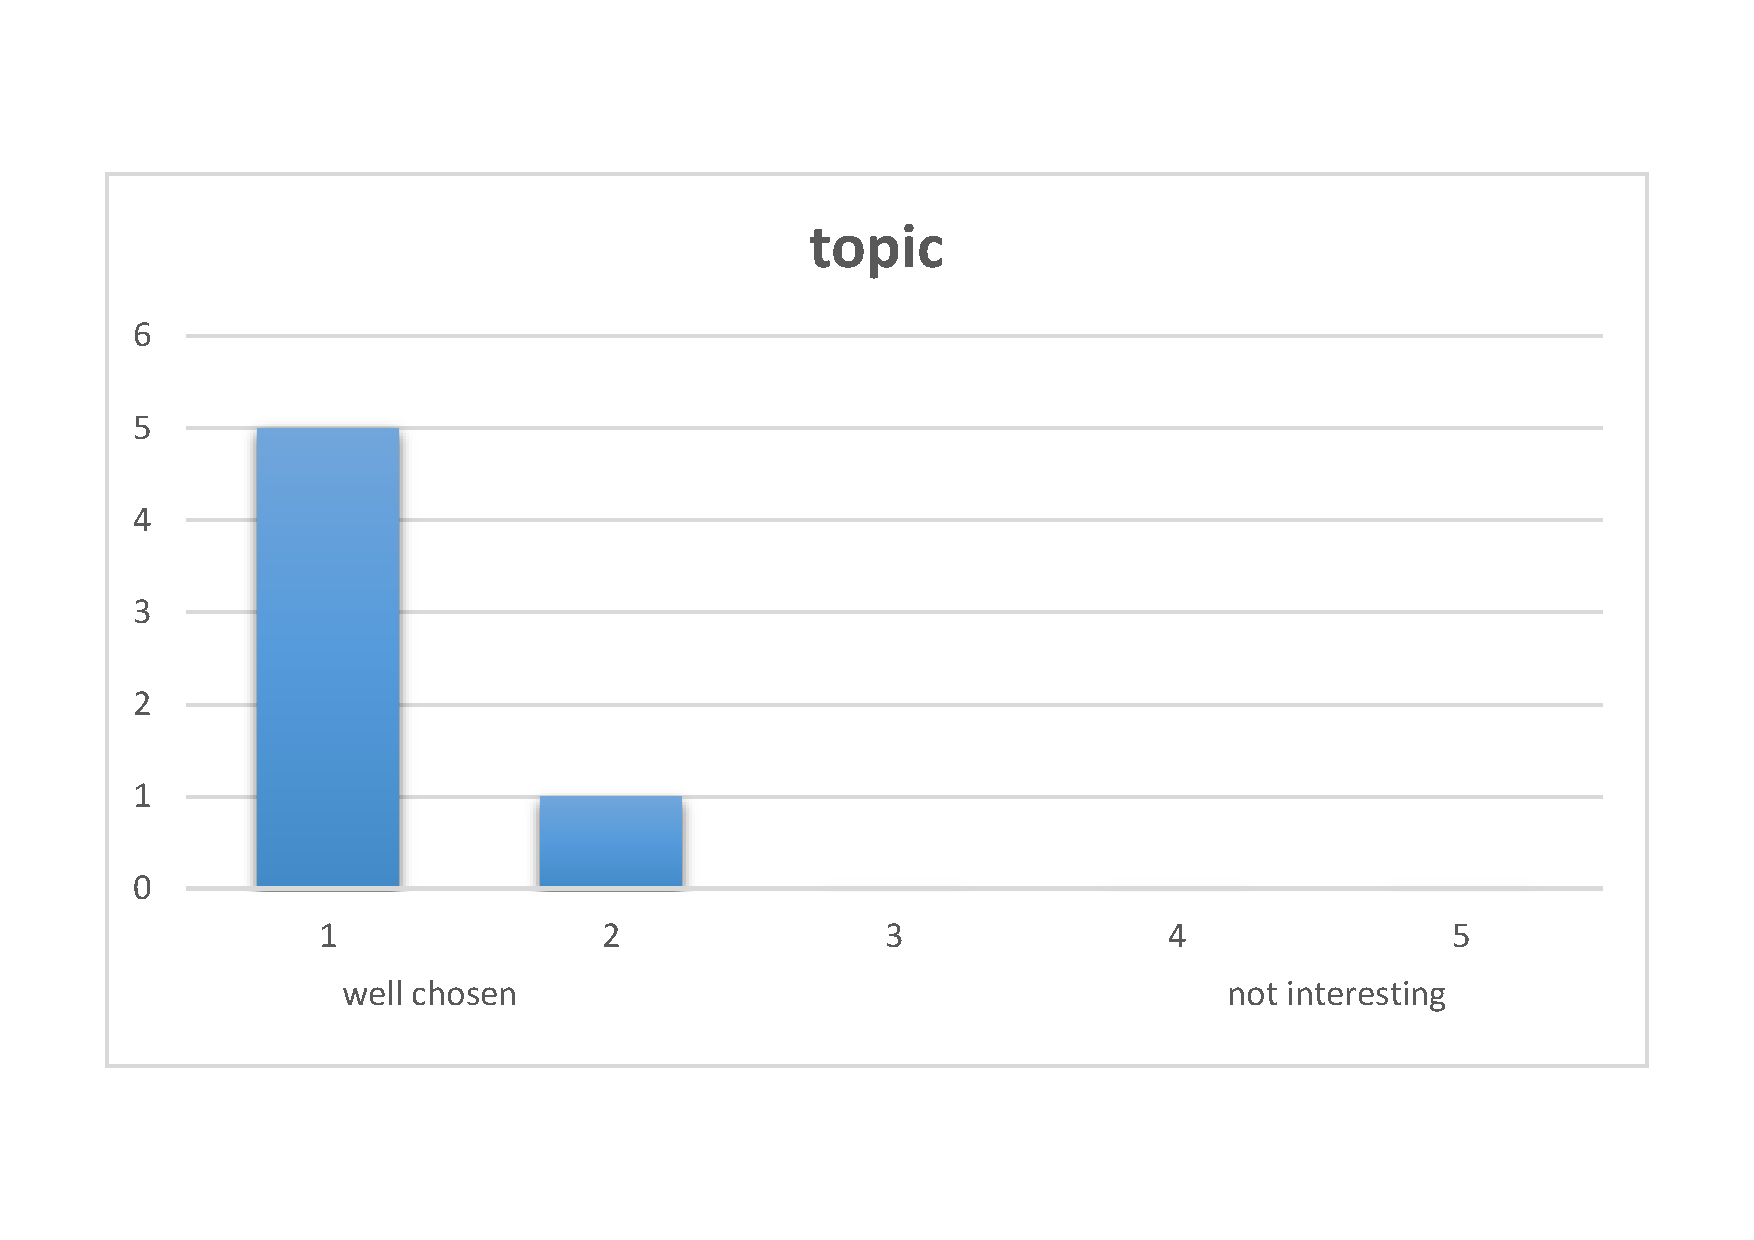
\includegraphics[width=0.5\textwidth]{eval/jendrzejewski/topic.pdf}}
\hfill %
\subfloat[\label{b}]{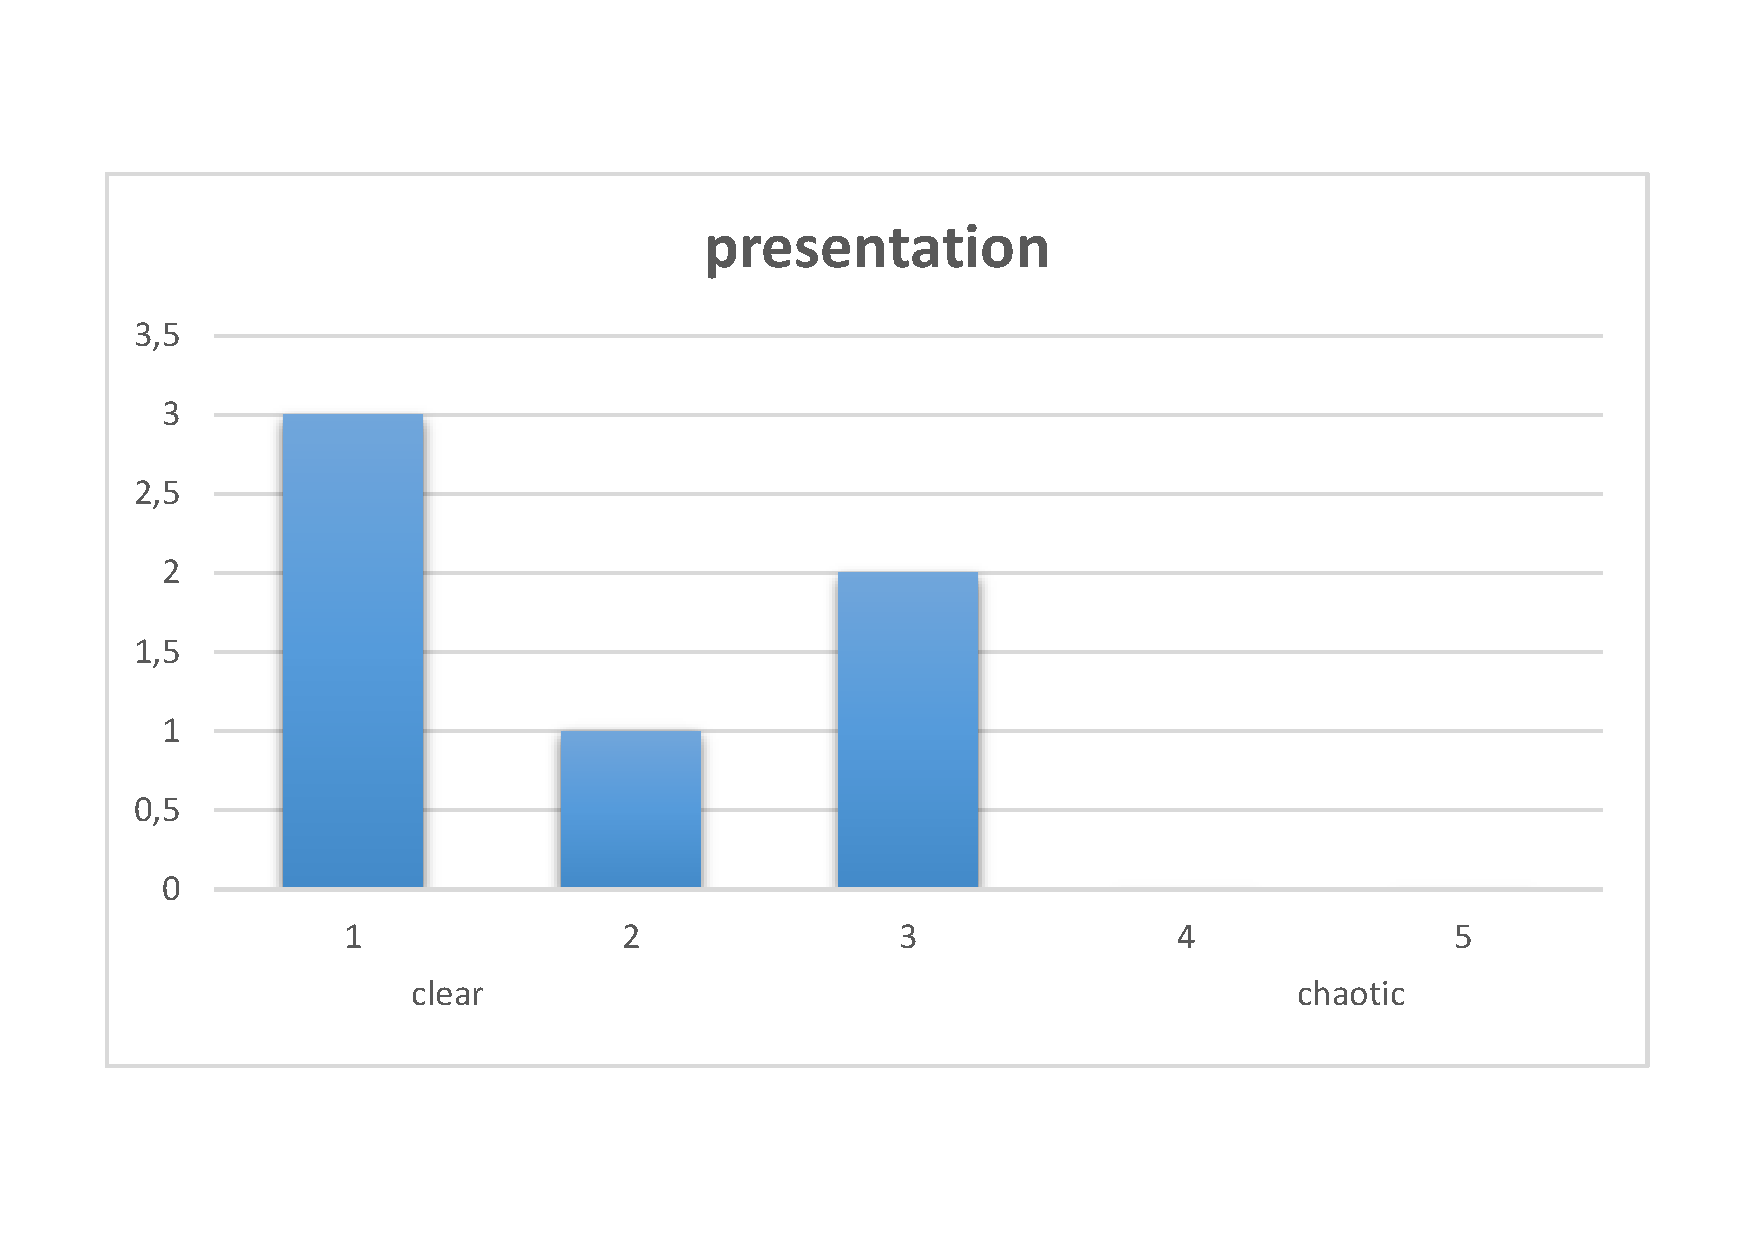
\includegraphics[width=0.5\textwidth]{eval/jendrzejewski/presentation.pdf}}
\hfill %
\subfloat[\label{b}]{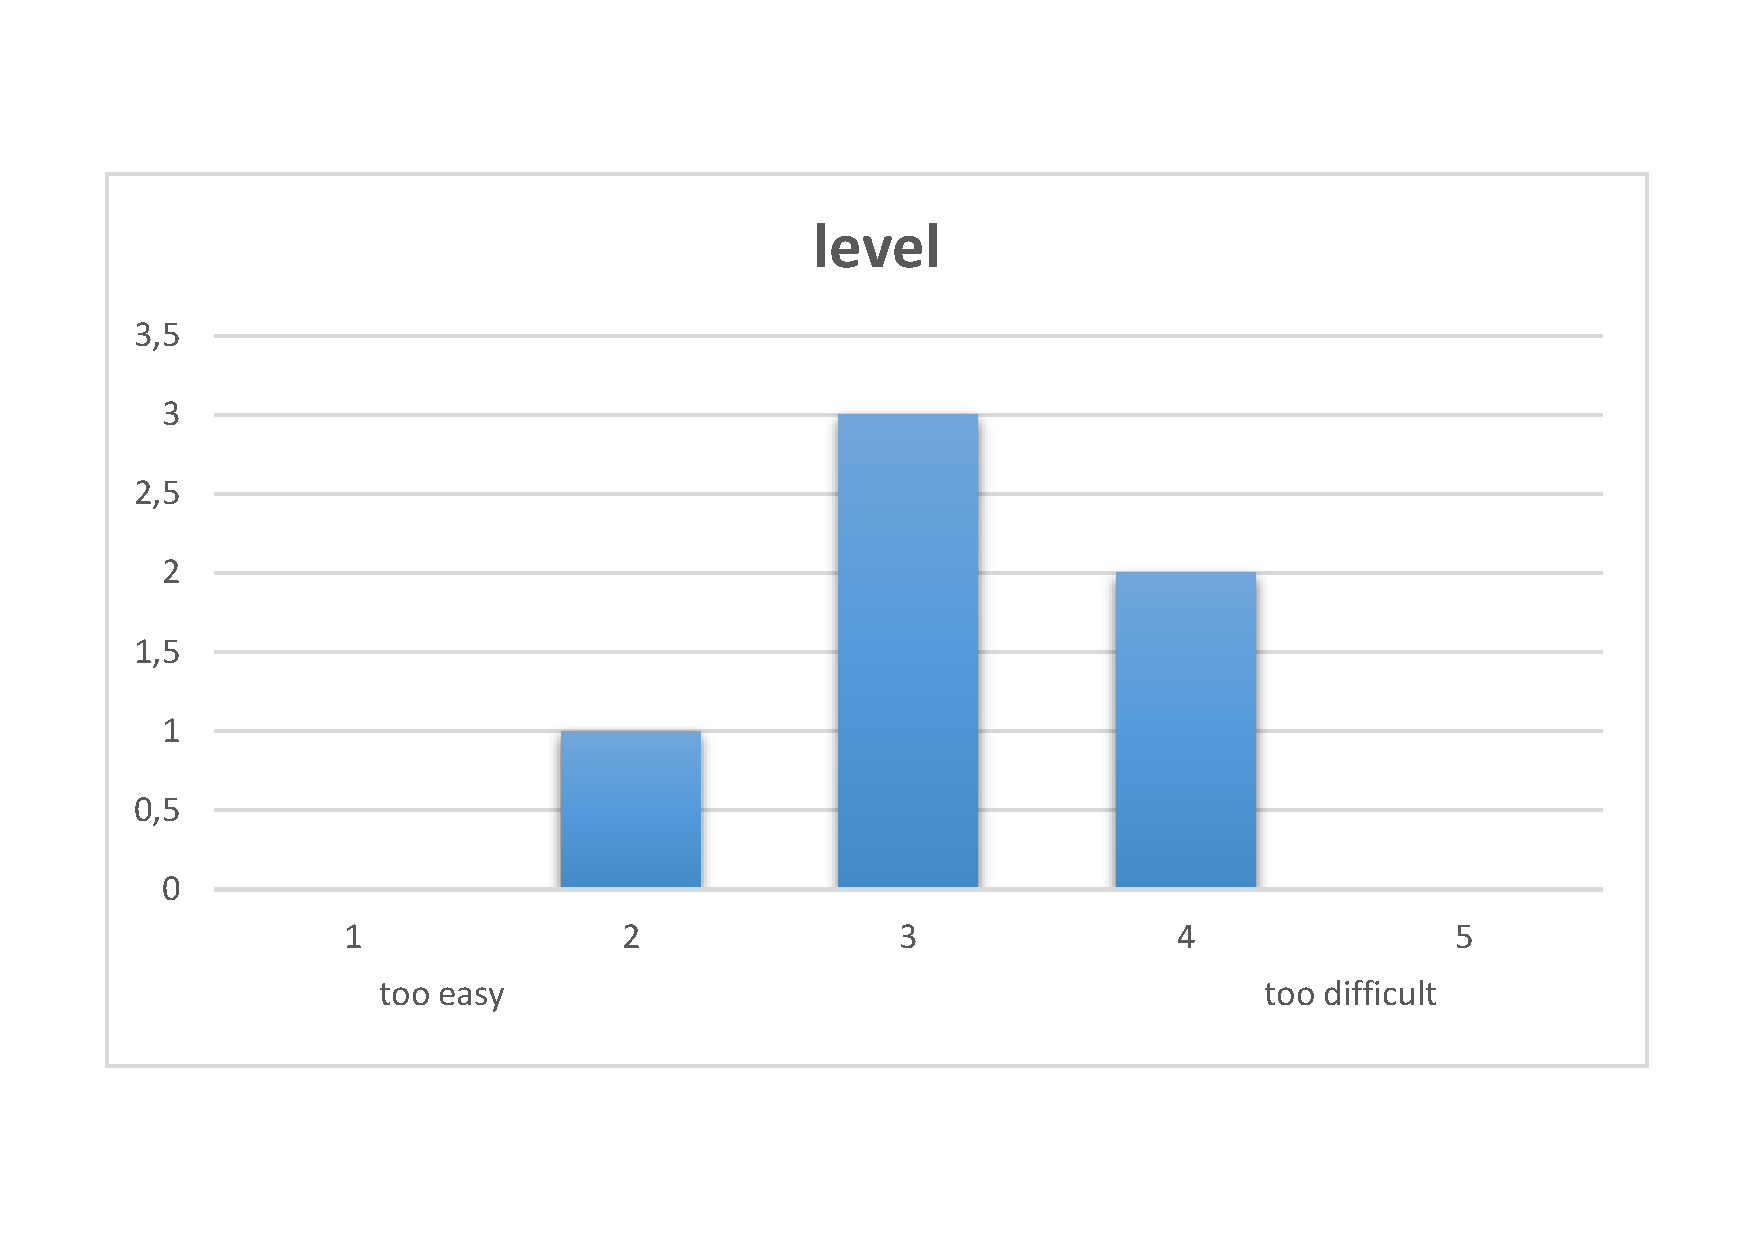
\includegraphics[width=0.5\textwidth]{eval/jendrzejewski/level.pdf}}
\hfill %
\subfloat[\label{b}]{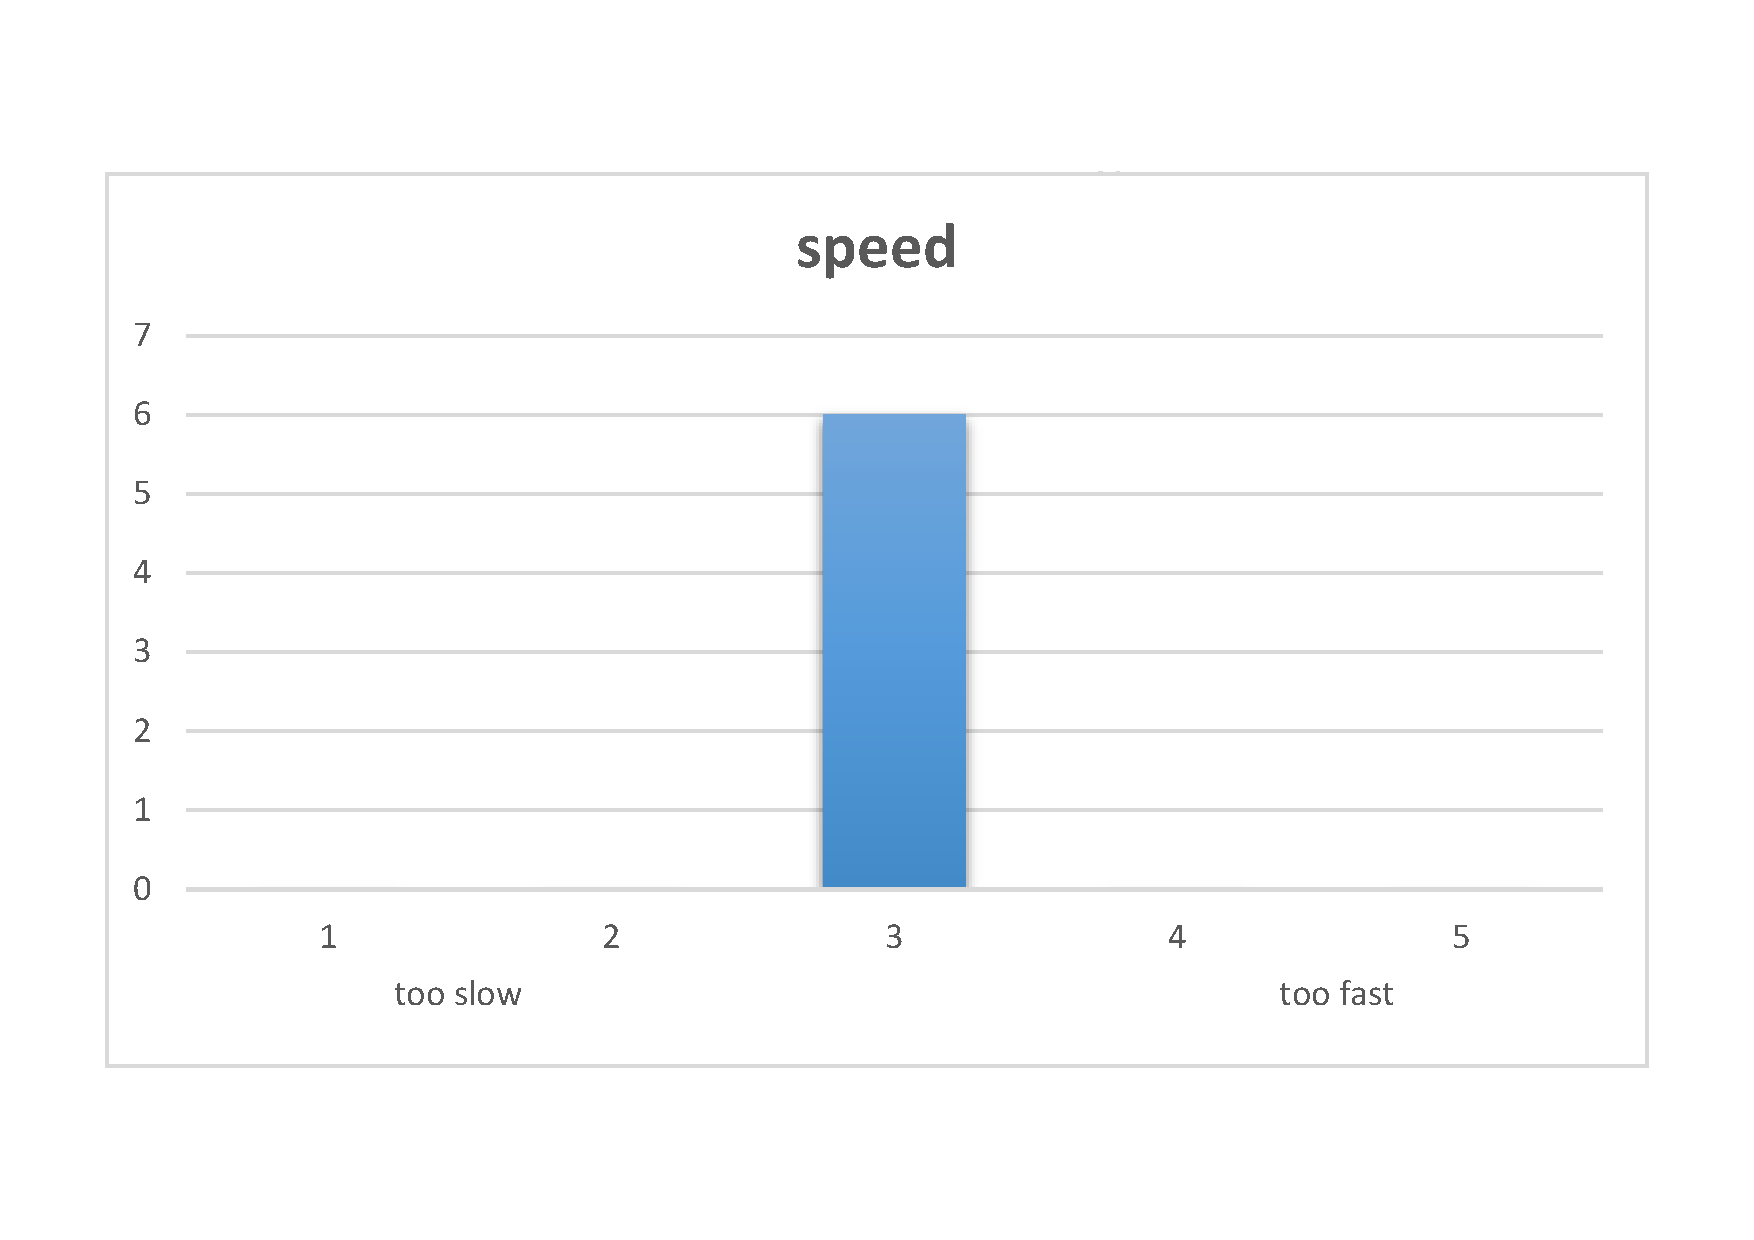
\includegraphics[width=0.5\textwidth]{eval/jendrzejewski/speed.pdf}}
\hfill\null % 
\caption{Lecture: F. Jendrzejewski - "Engineering static and dynamical gauge fields with ultracold matter"}
\end{figure}

\subsubsection{Lecture: G. Parmentier - "Star Clusters and Star Cluster Systems"}

\begin{figure}[H]
\centering
\null\hfill %
\subfloat[\label{b}]{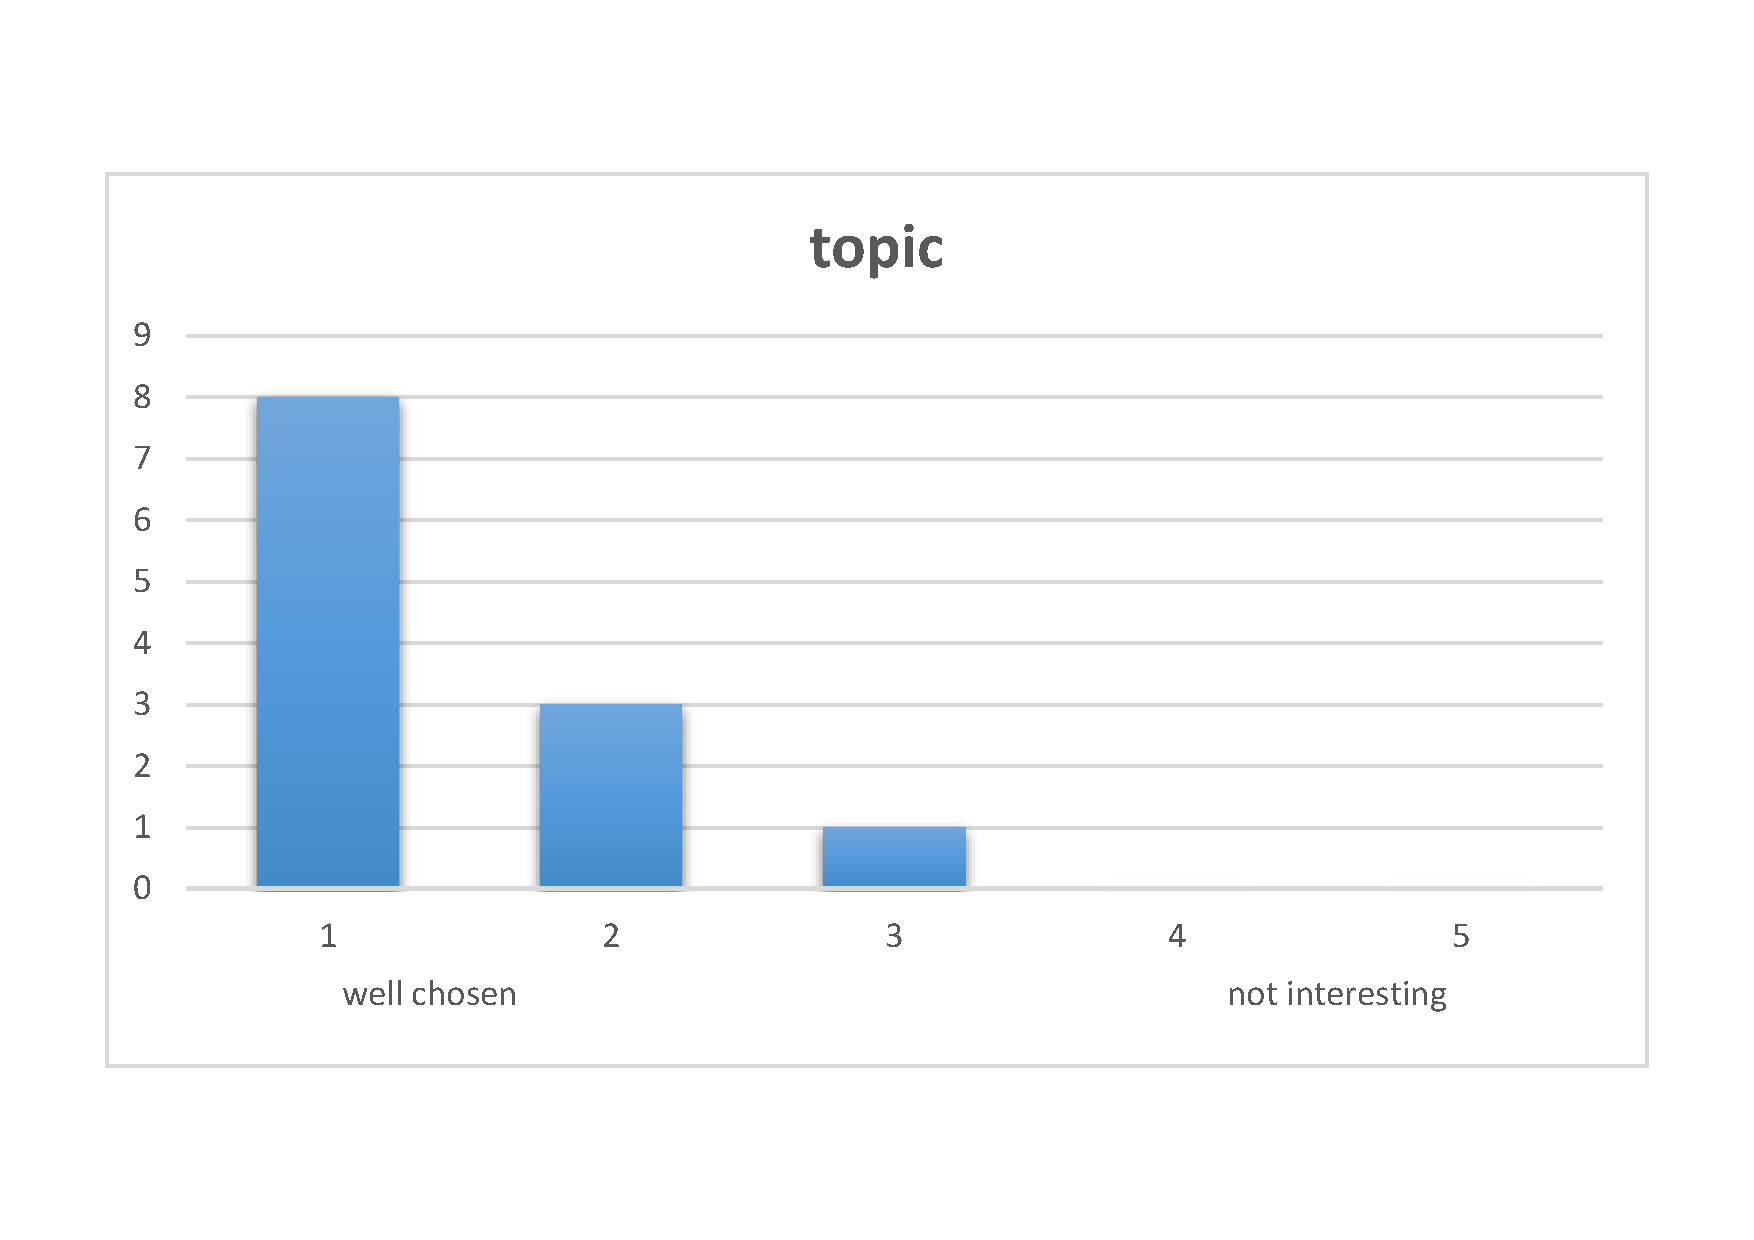
\includegraphics[width=0.5\textwidth]{eval/parmentier/topic.pdf}}
\hfill %
\subfloat[\label{b}]{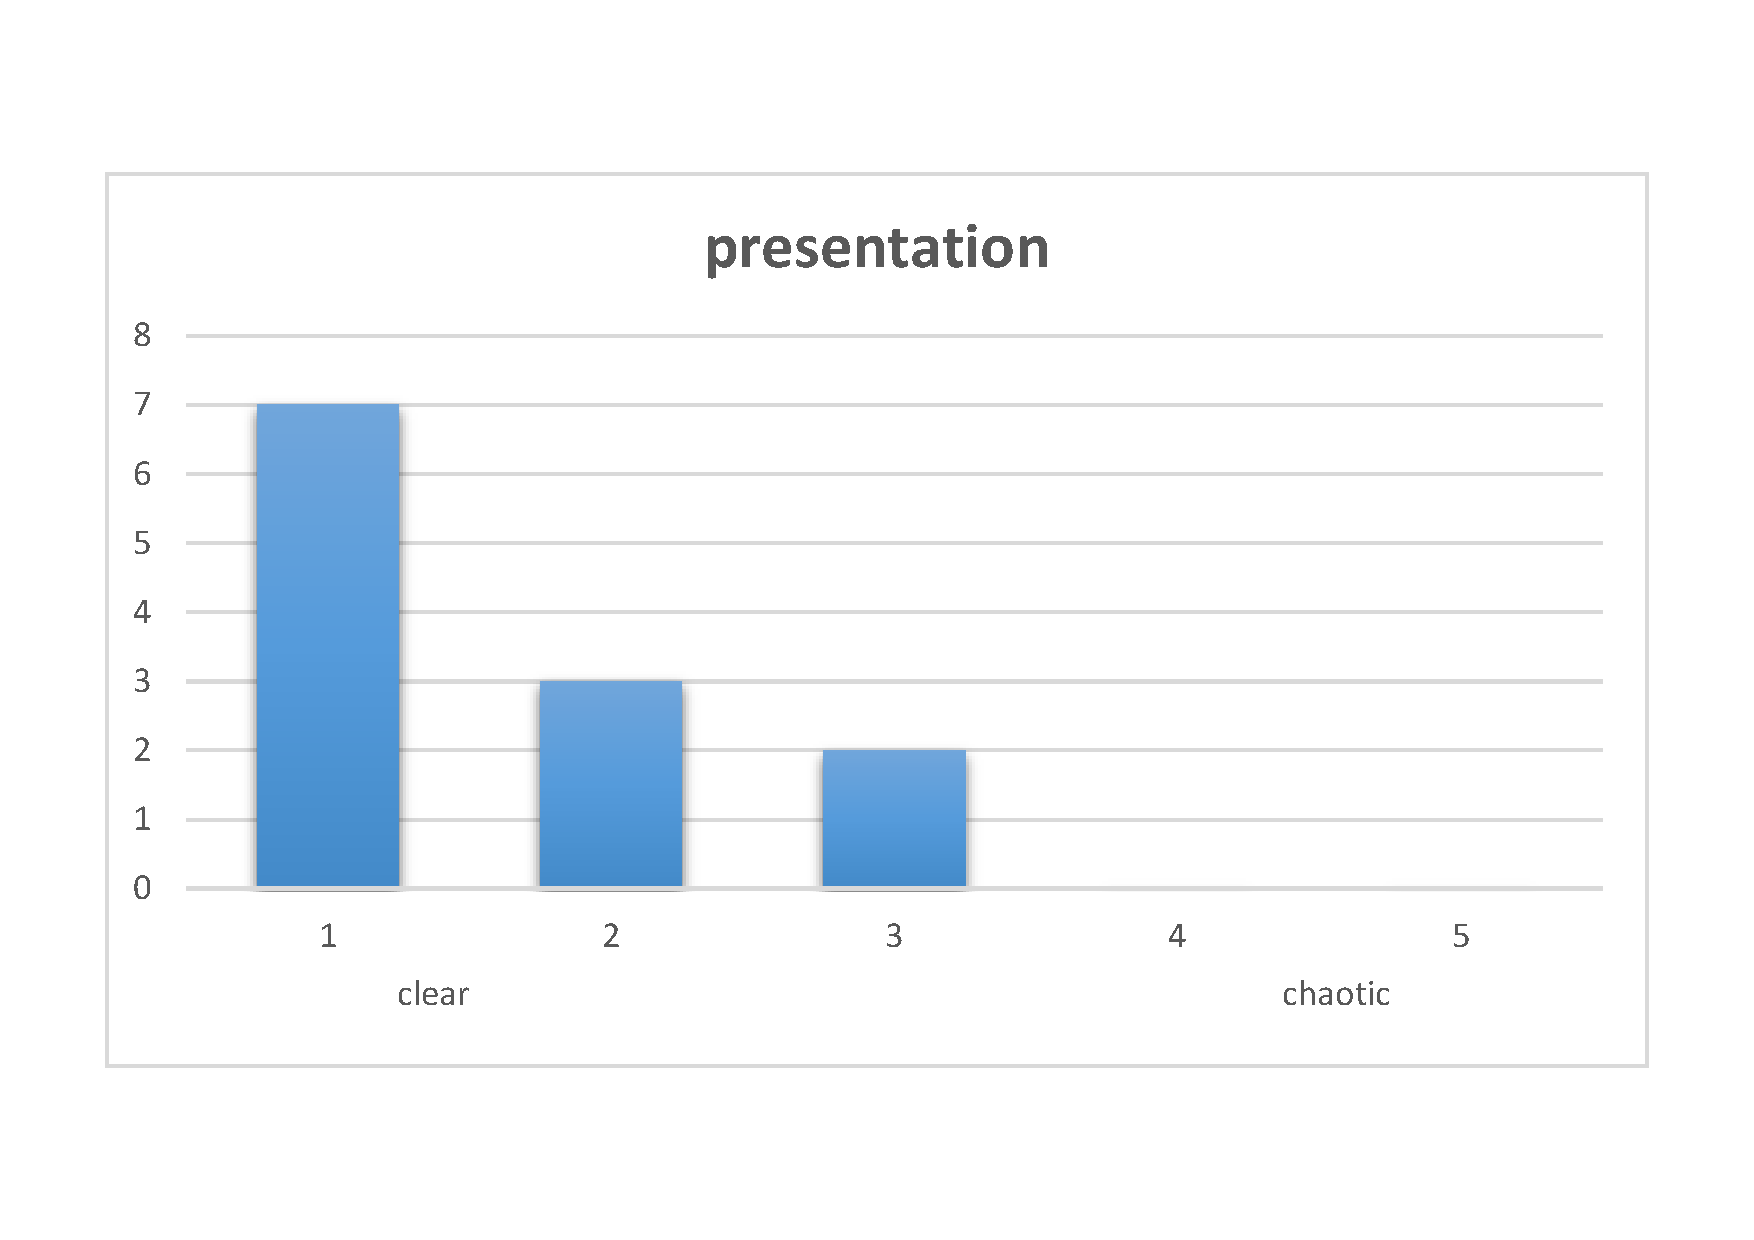
\includegraphics[width=0.5\textwidth]{eval/parmentier/presentation.pdf}}
\hfill %
\subfloat[\label{b}]{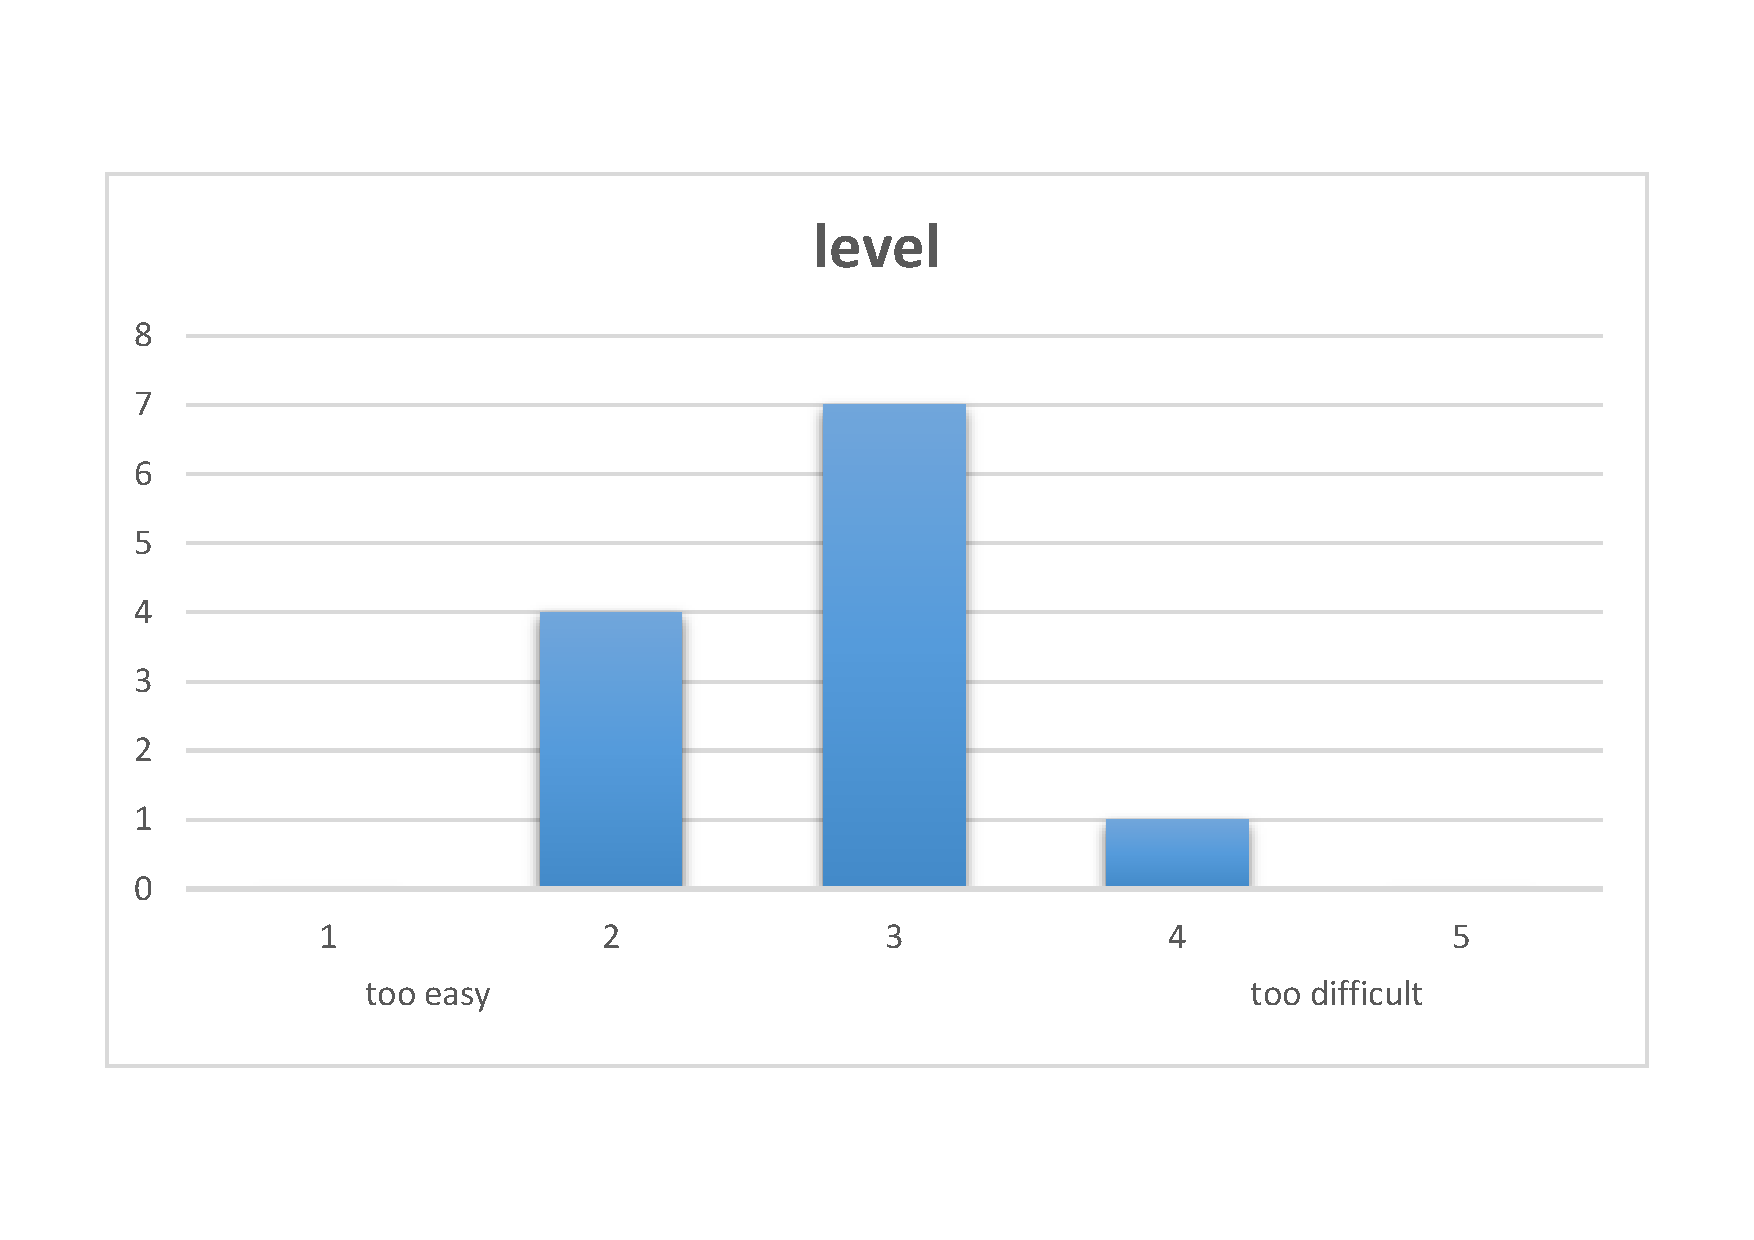
\includegraphics[width=0.5\textwidth]{eval/parmentier/level.pdf}}
\hfill %
\subfloat[\label{b}]{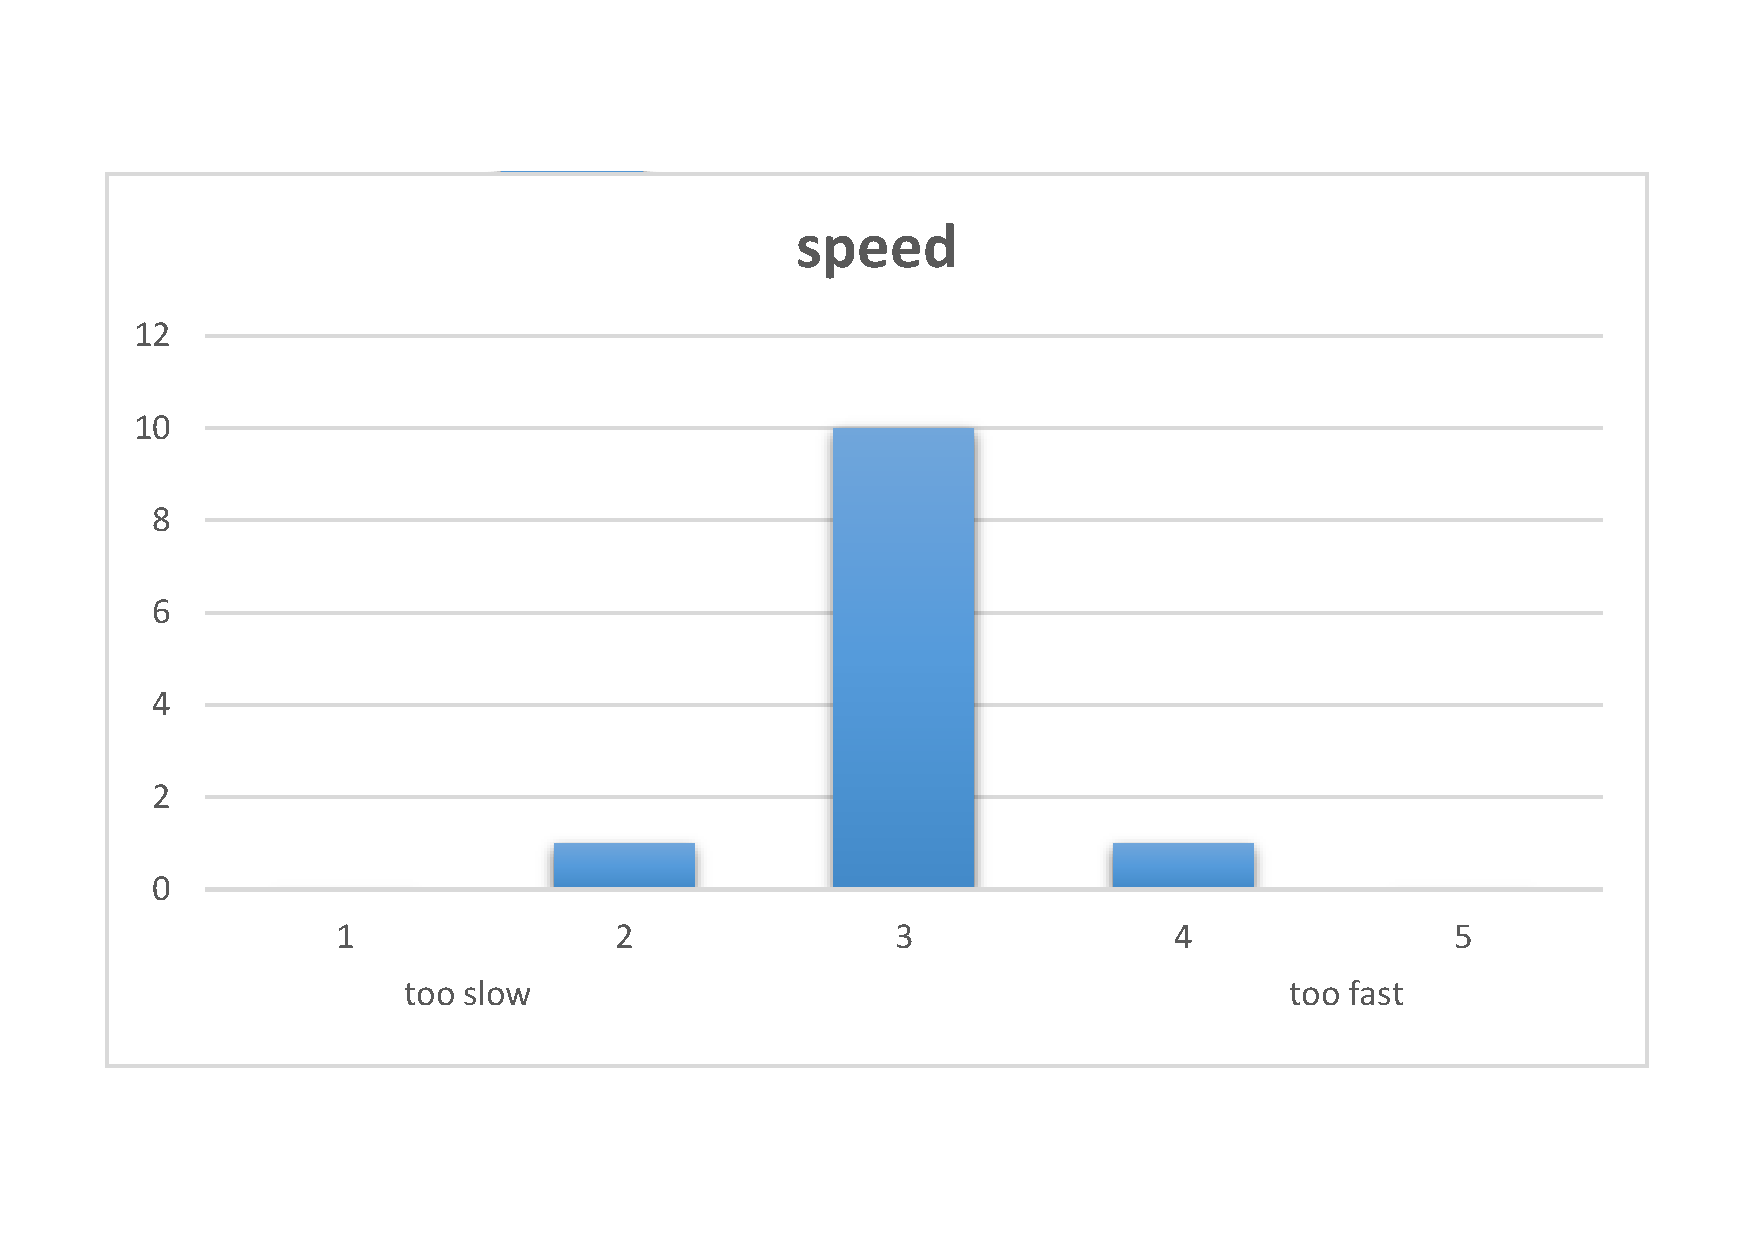
\includegraphics[width=0.5\textwidth]{eval/parmentier/speed.pdf}}
\hfill\null % 
\caption{Lecture: G. Parmentier - "Star Clusters and Star Cluster Systems"}
\end{figure}

\subsubsection{Lecture: B. M. Sch\"afer - "Fundamental principles and their realisation in physical laws"}

\begin{figure}[H]
\centering
\null\hfill %
\subfloat[\label{b}]{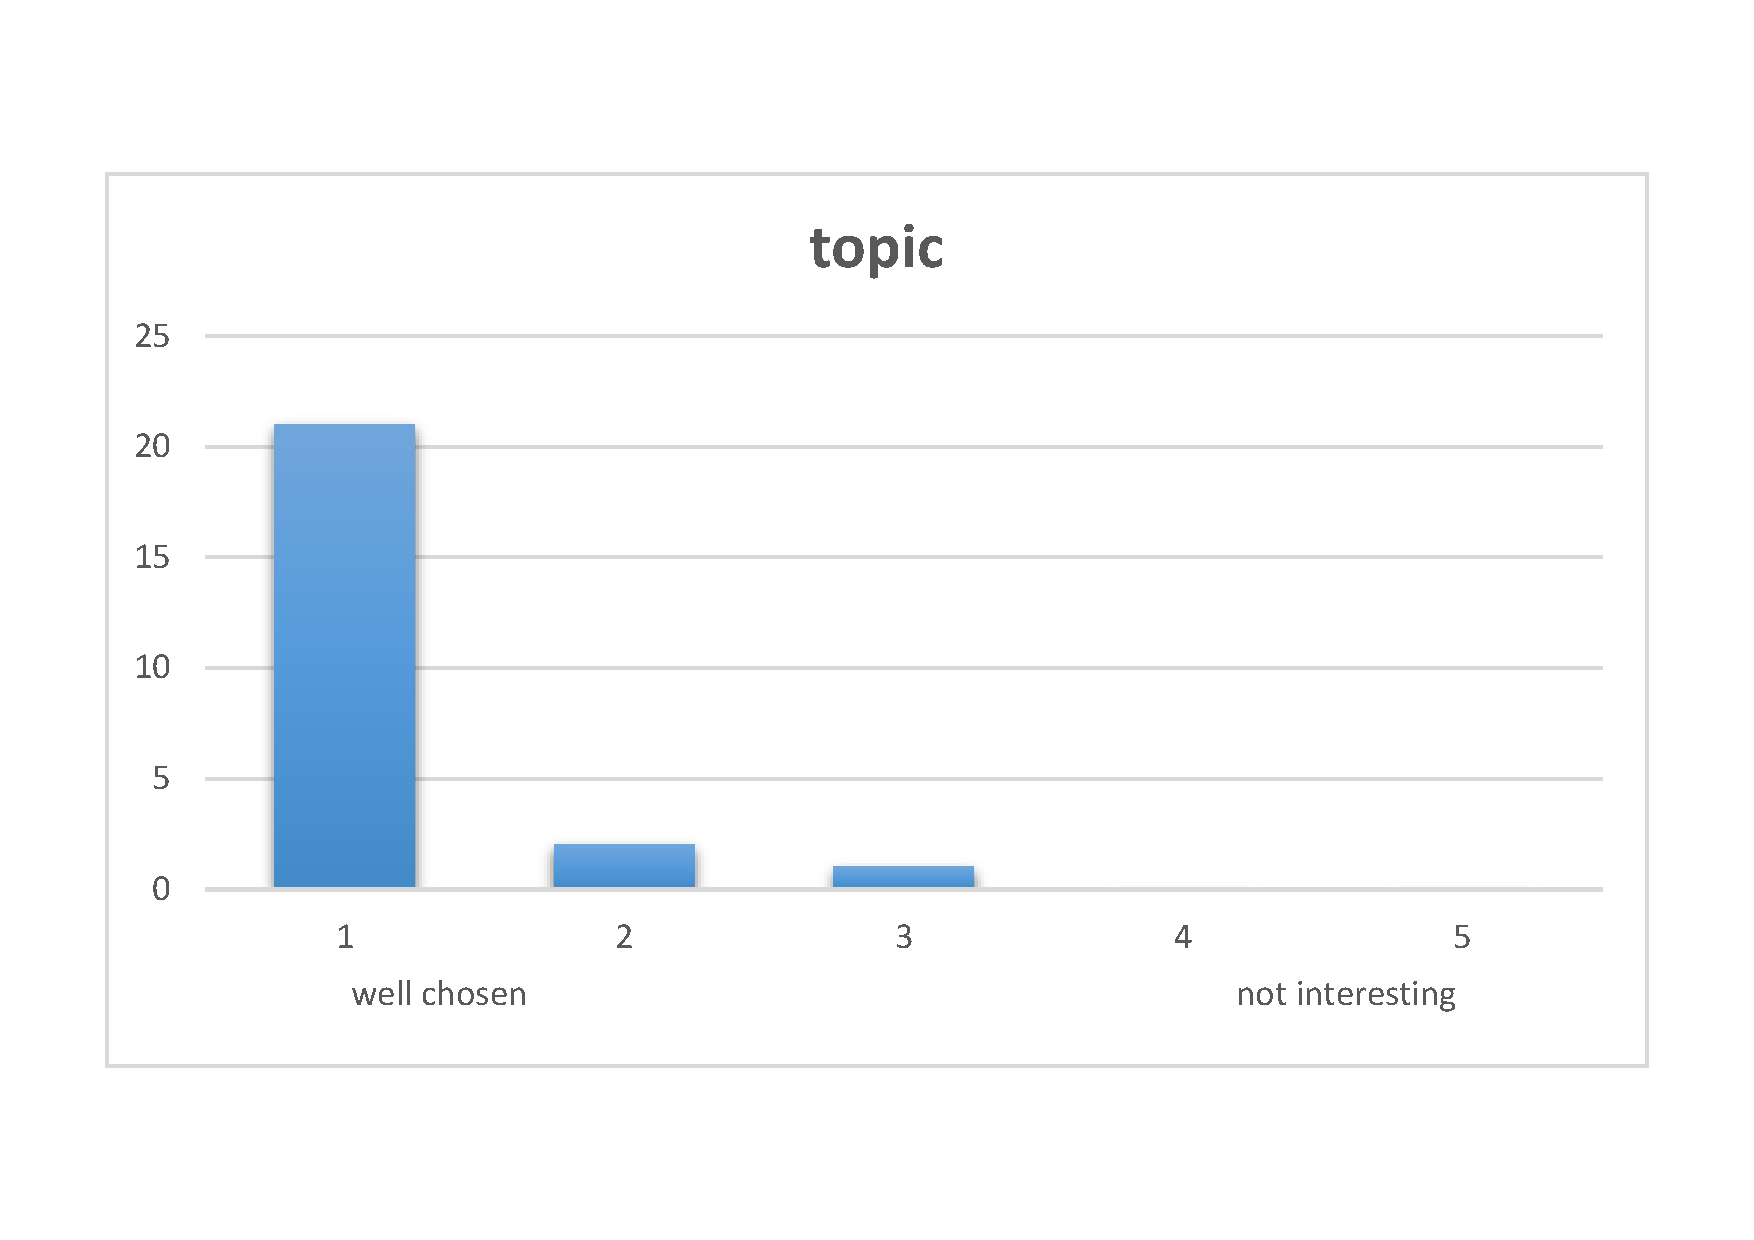
\includegraphics[width=0.5\textwidth]{eval/schaefer/topic.pdf}}
\hfill %
\subfloat[\label{b}]{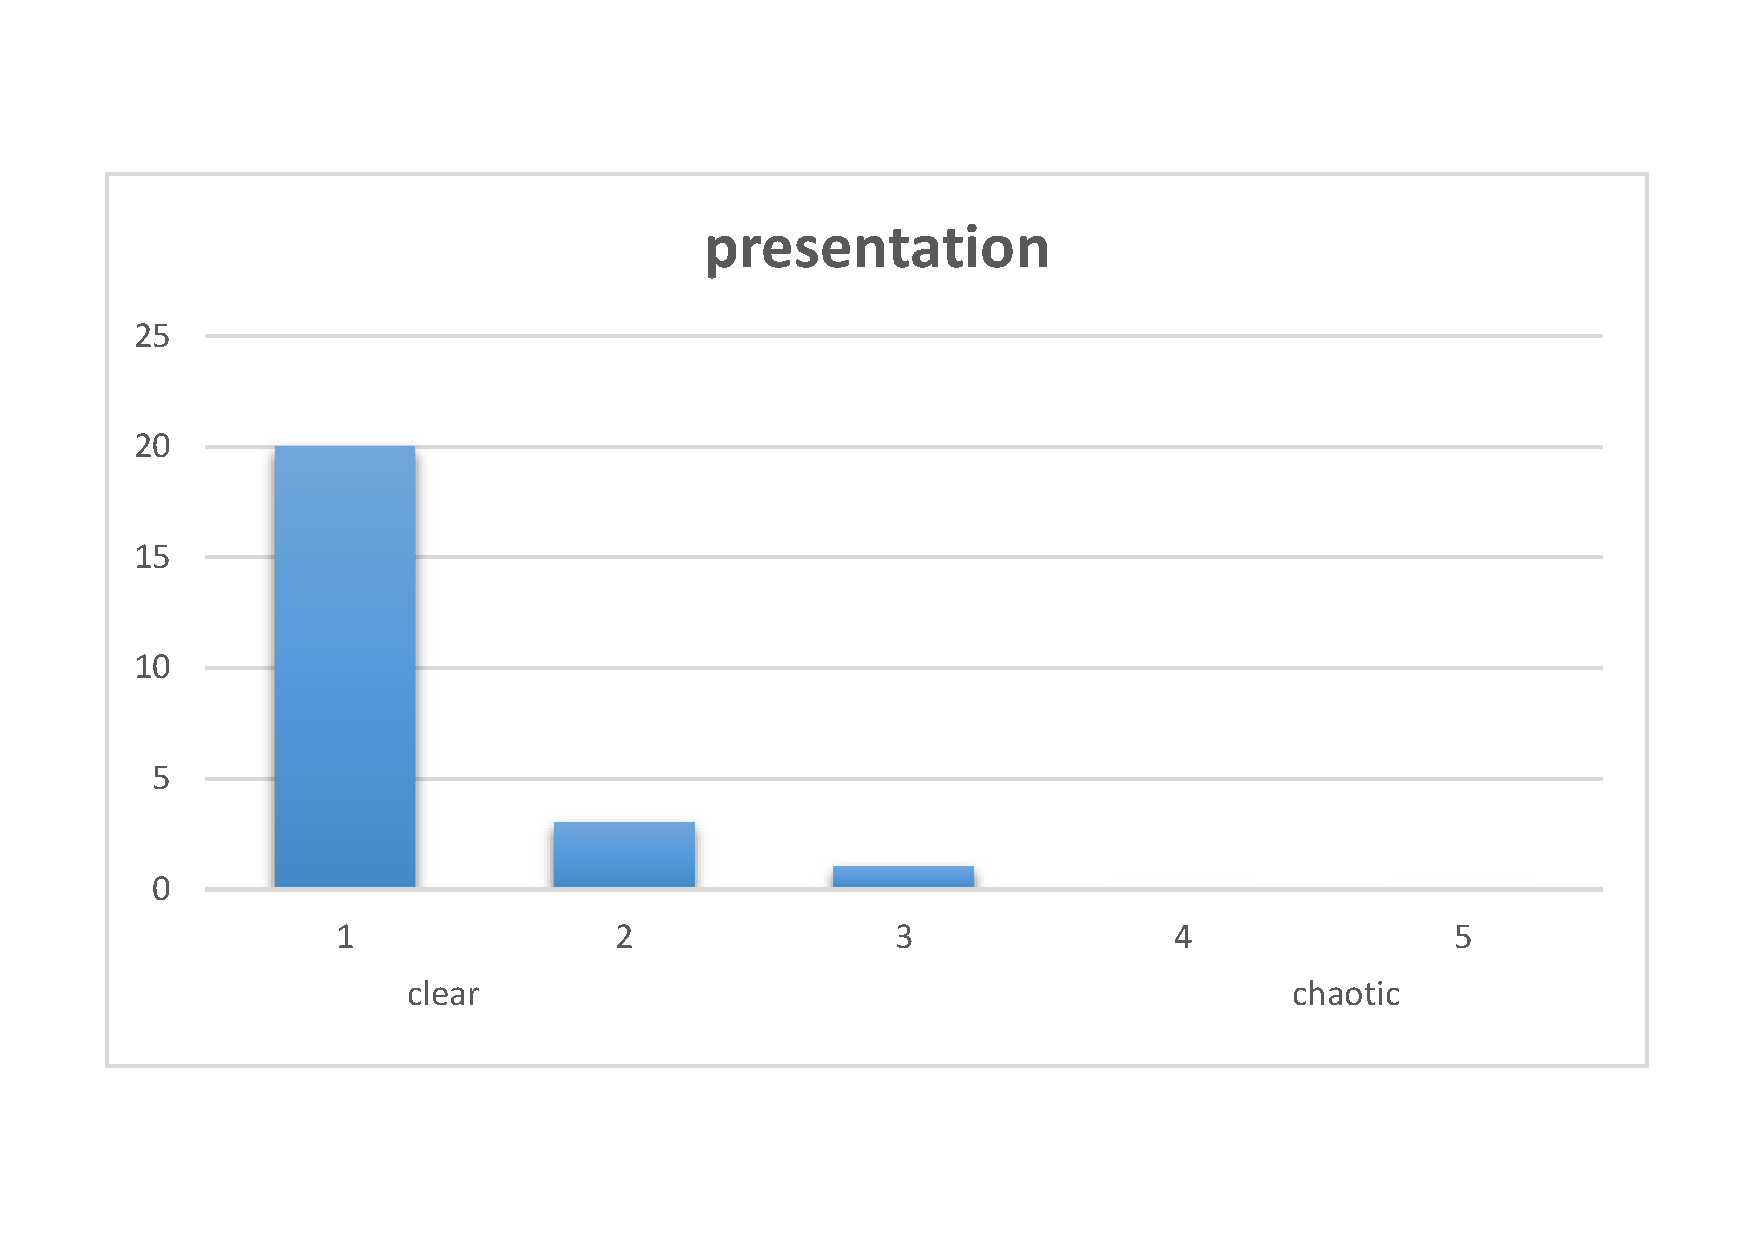
\includegraphics[width=0.5\textwidth]{eval/schaefer/presentation.pdf}}
\hfill %
\subfloat[\label{b}]{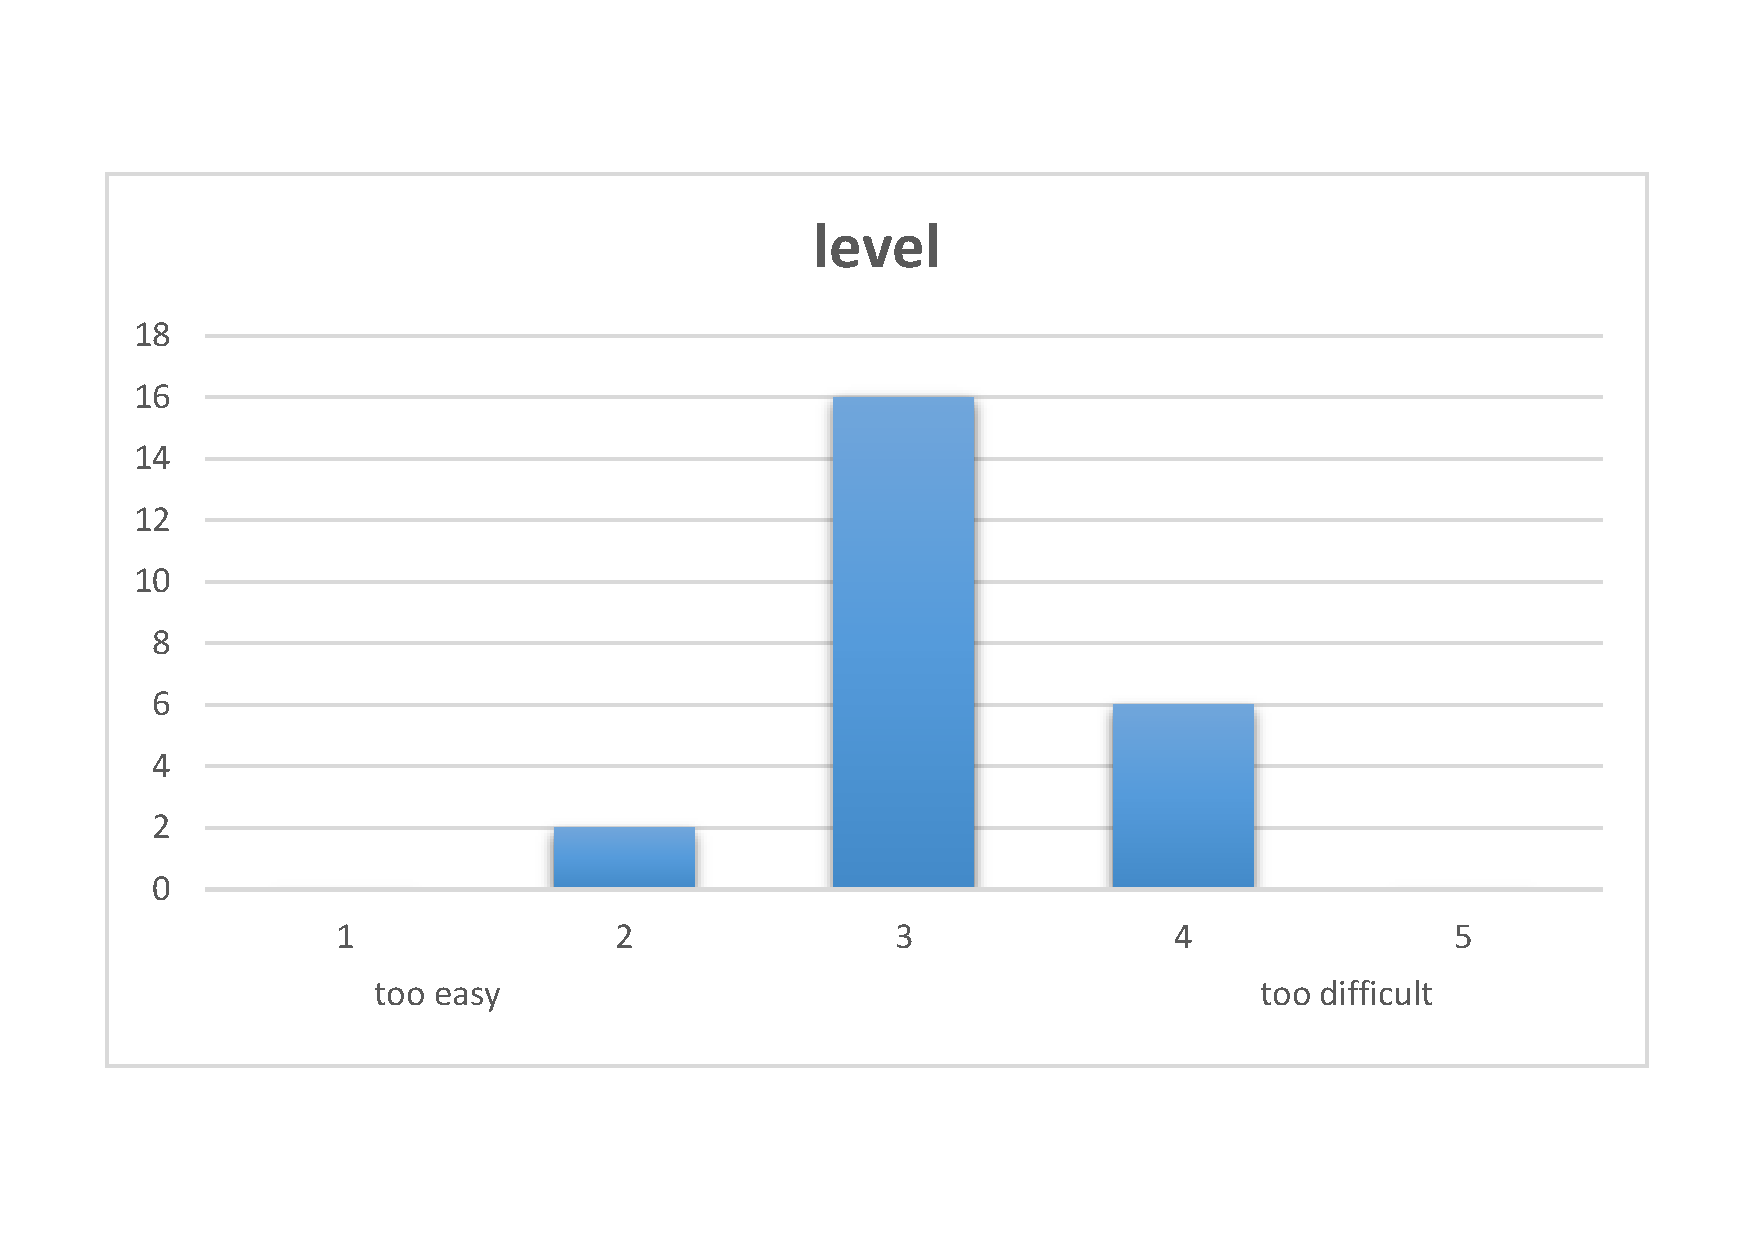
\includegraphics[width=0.5\textwidth]{eval/schaefer/level.pdf}}
\hfill %
\subfloat[\label{b}]{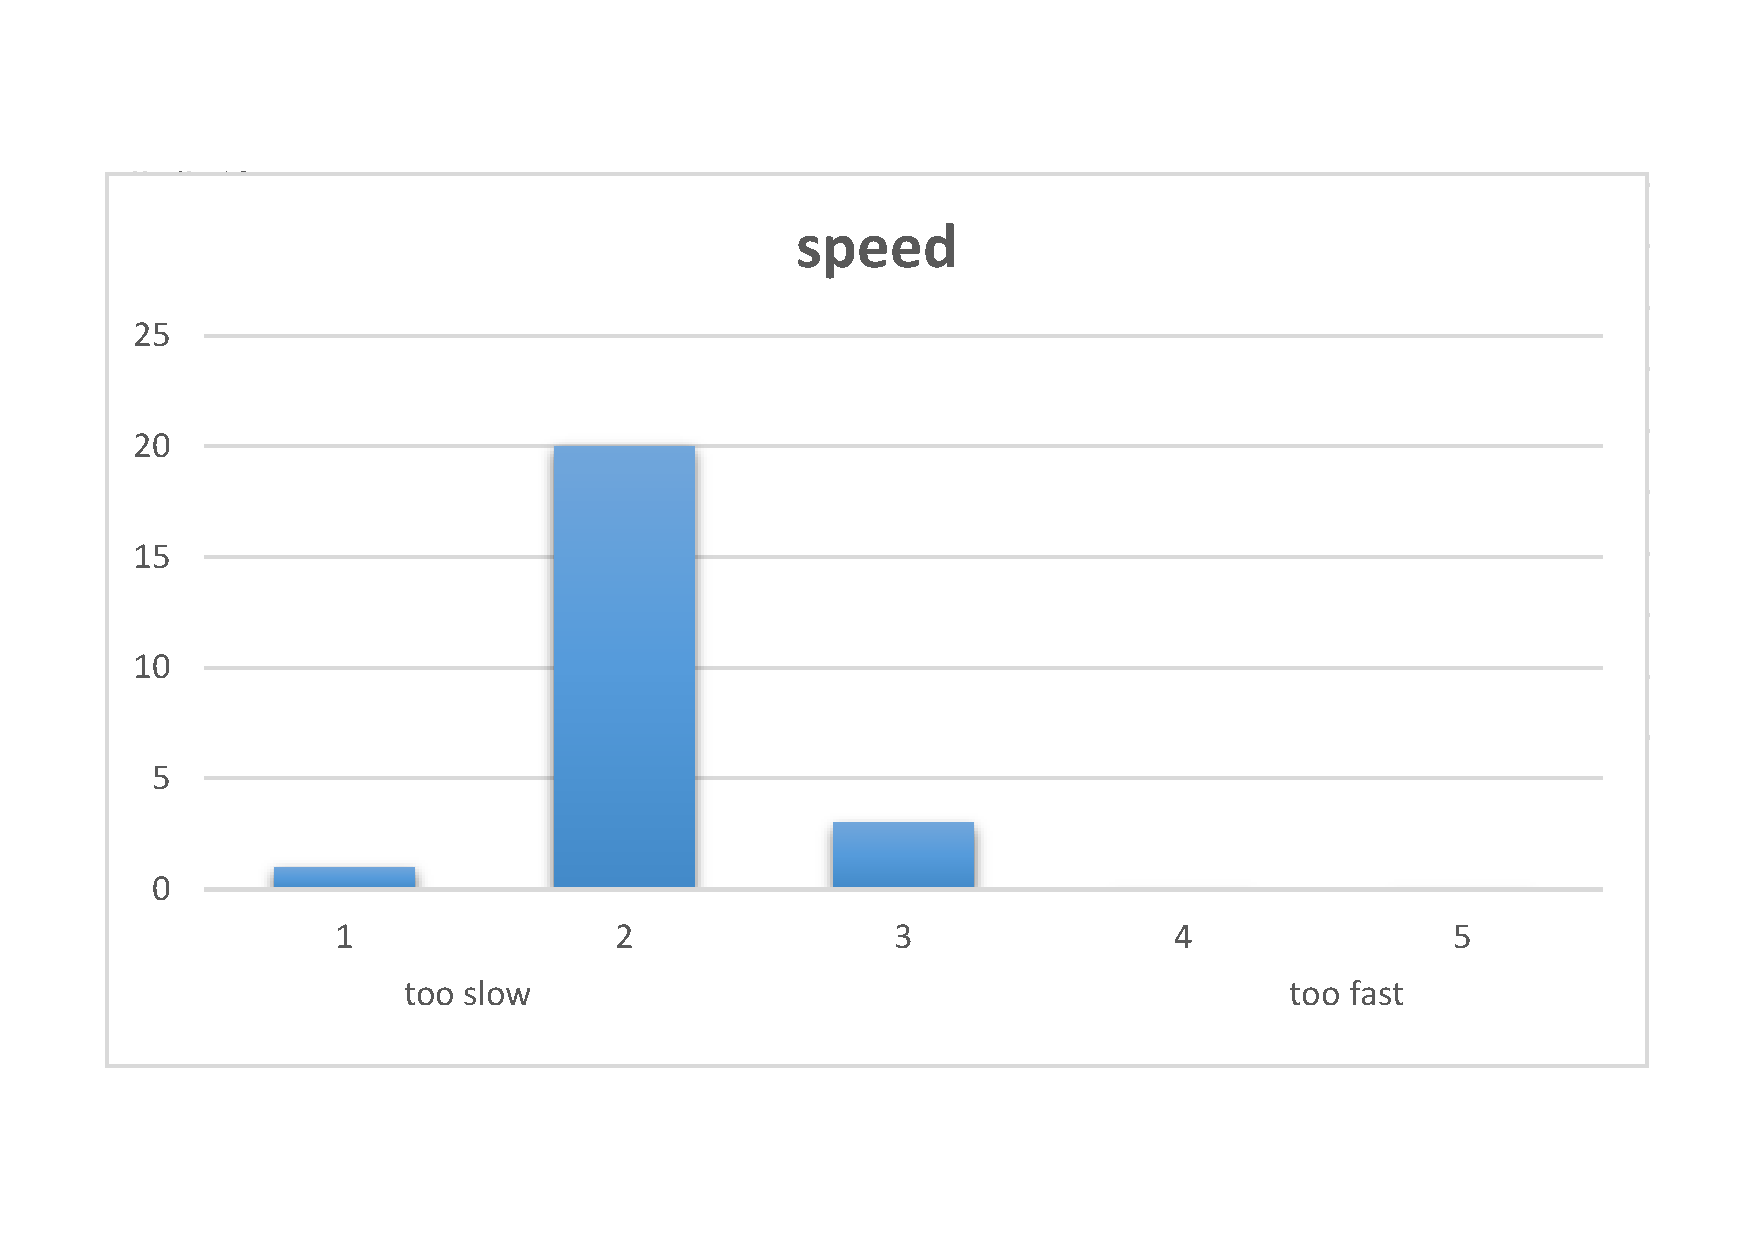
\includegraphics[width=0.5\textwidth]{eval/schaefer/speed.pdf}}
\hfill\null % 
\caption{Lecture: B. M. Sch\"afer - "Fundamental principles and their realisation in physical laws"}
\end{figure}

\subsubsection{Lecture: L. Witkowski - "Folk Theorems of Quantum Gravity"}

\begin{figure}[H]
\centering
\null\hfill %
\subfloat[\label{b}]{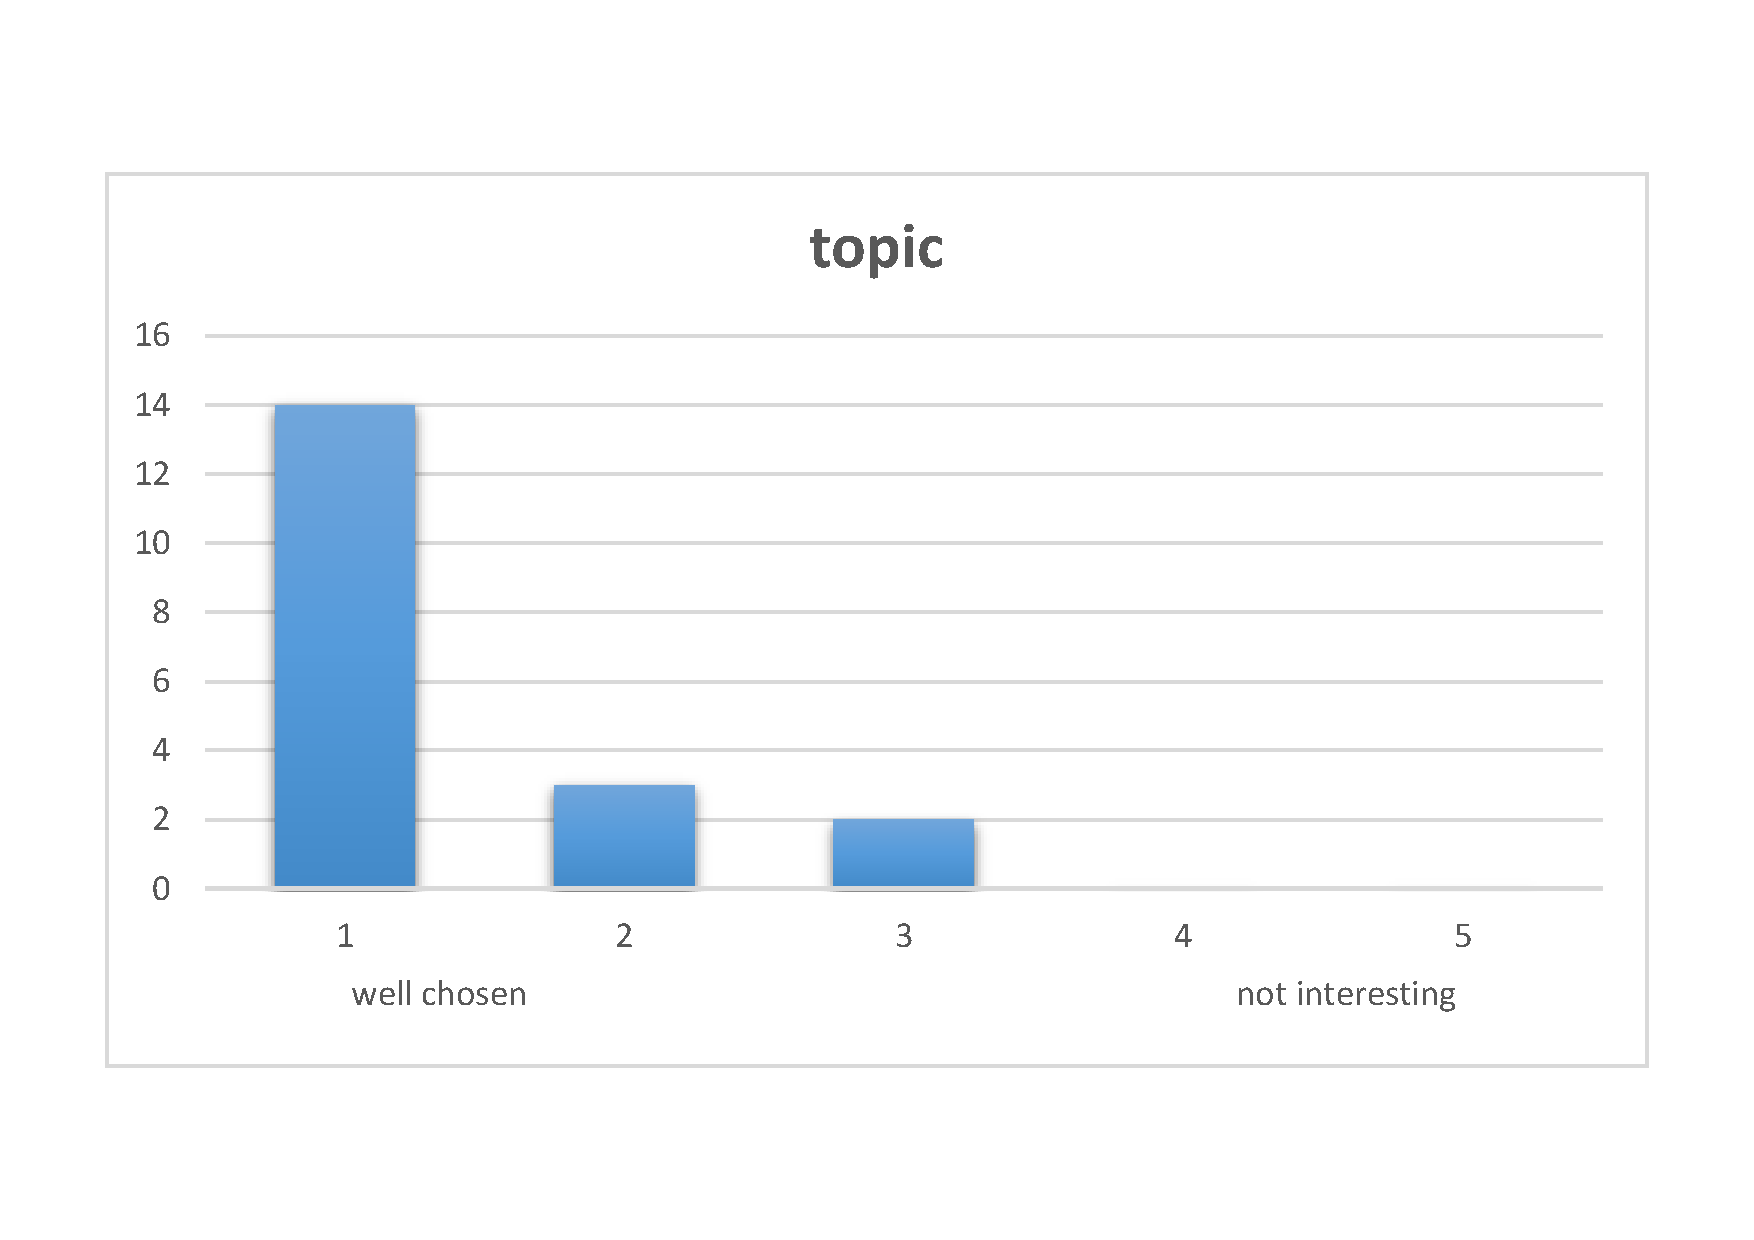
\includegraphics[width=0.5\textwidth]{eval/witkowski/topic.pdf}}
\hfill %
\subfloat[\label{b}]{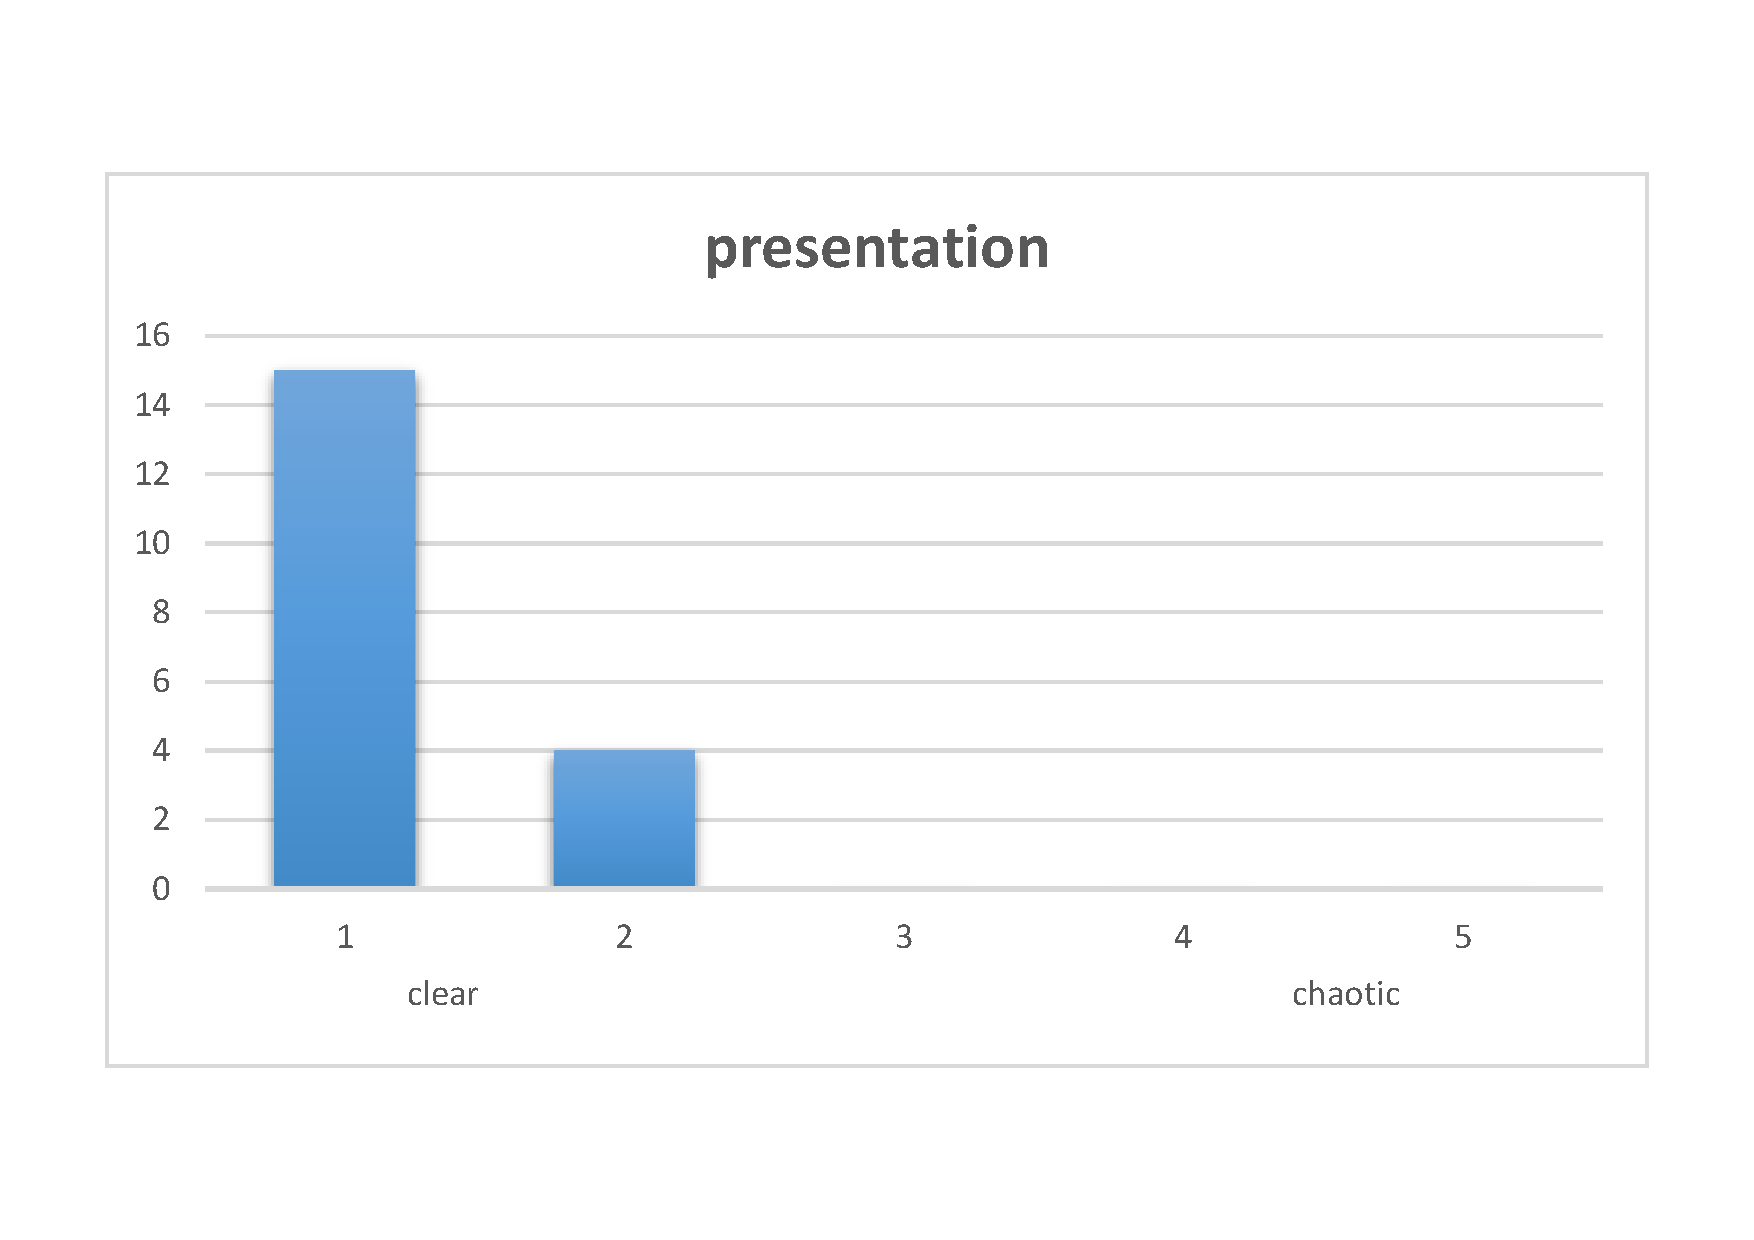
\includegraphics[width=0.5\textwidth]{eval/witkowski/presentation.pdf}}
\hfill %
\subfloat[\label{b}]{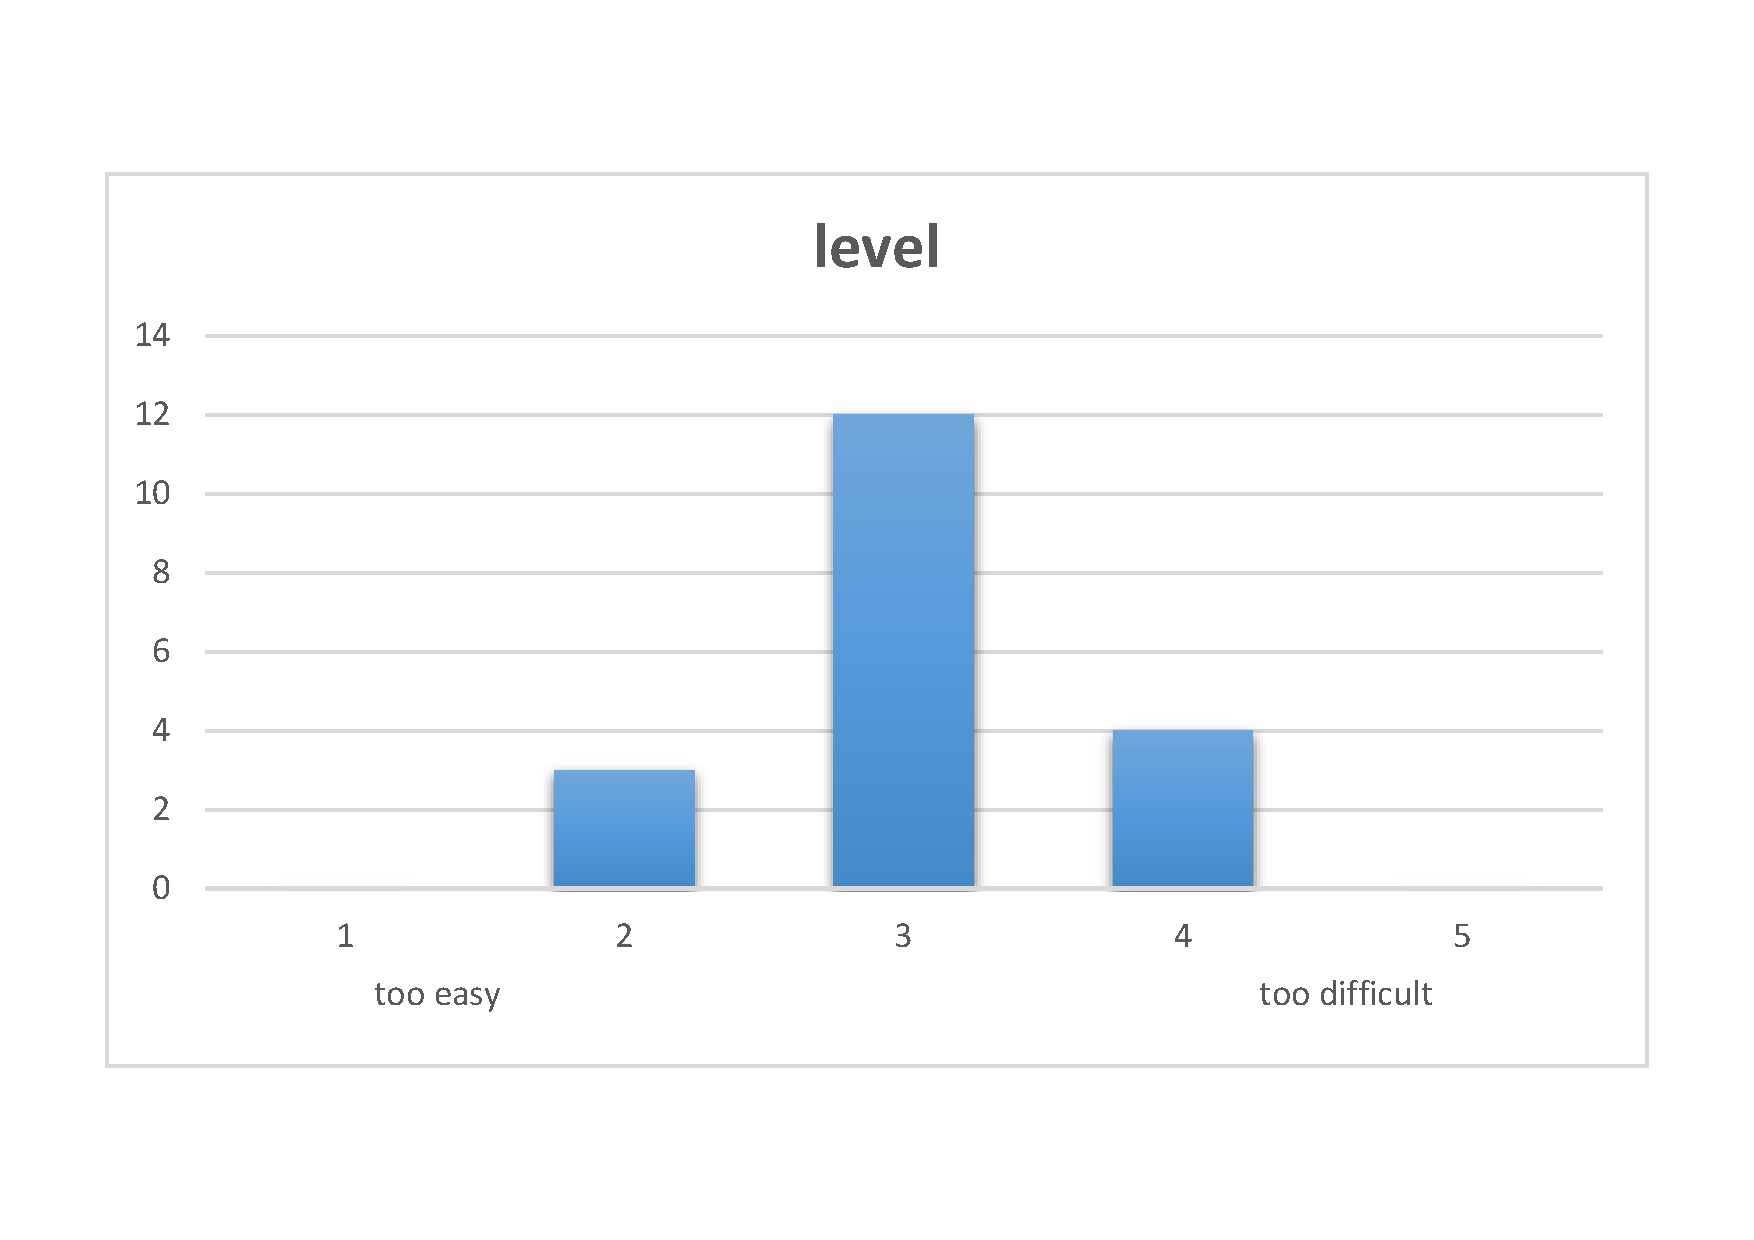
\includegraphics[width=0.5\textwidth]{eval/witkowski/level.pdf}}
\hfill %
\subfloat[\label{b}]{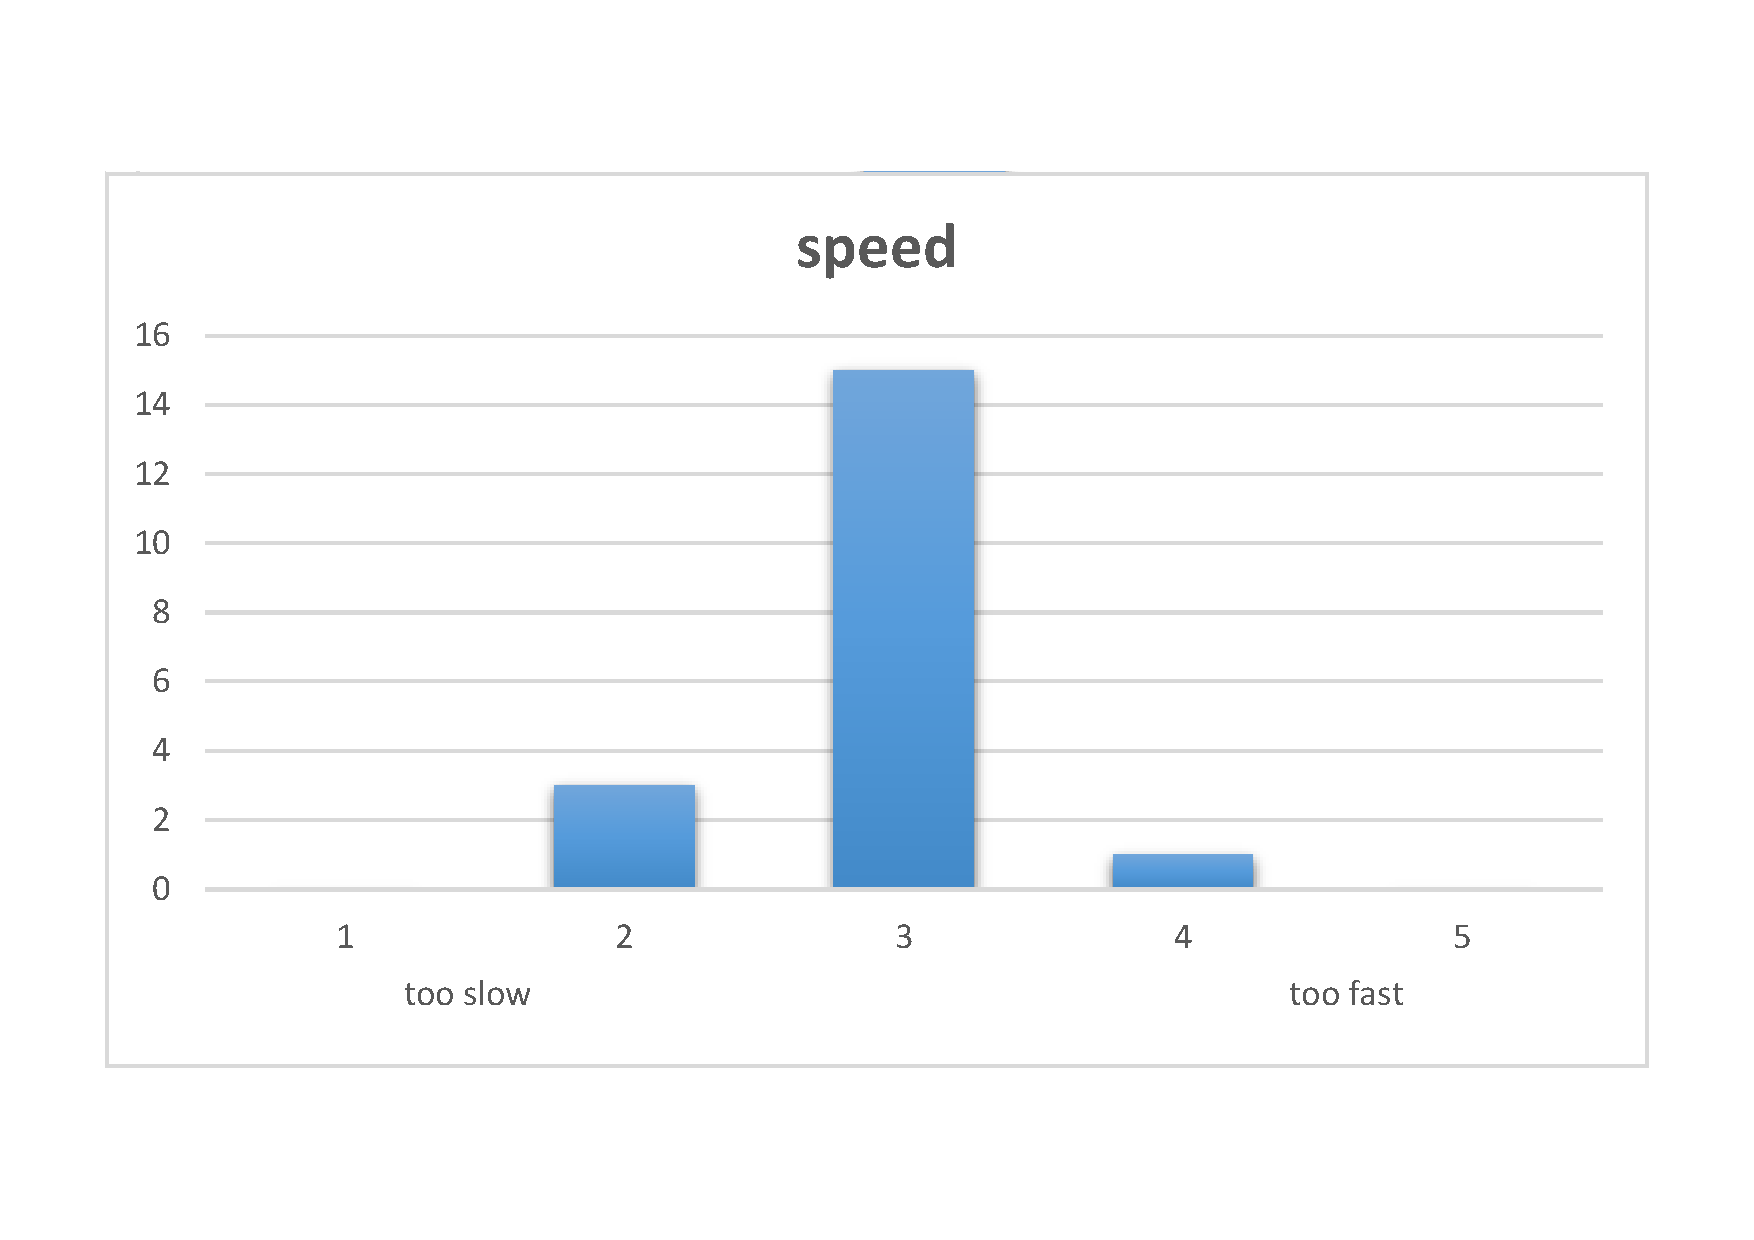
\includegraphics[width=0.5\textwidth]{eval/witkowski/speed.pdf}}
\hfill\null % 
\caption{Lecture: L. Witkowski - "Folk Theorems of Quantum
Gravity"}
\end{figure}

\subsubsection{Lecture: P. Yogeshwar - "Environmental Geophysics using Electromagnetic Methods"}

\begin{figure}[H]
\centering
\null\hfill %
\subfloat[\label{b}]{\includegraphics[width=0.5\textwidth]{eval/yogeshwar/topic.pdf}}
\hfill %
\subfloat[\label{b}]{\includegraphics[width=0.5\textwidth]{eval/yogeshwar/presentation.pdf}}
\hfill %
\subfloat[\label{b}]{\includegraphics[width=0.5\textwidth]{eval/yogeshwar/level.pdf}}
\hfill %
\subfloat[\label{b}]{\includegraphics[width=0.5\textwidth]{eval/yogeshwar/speed.pdf}}
\hfill\null % 
\caption{Lecture: P. Yogeshwar - "Environmental Geophysics using Electromagnetic Methods"}
\end{figure}

\newpage

\subsection{Comments from participants: What did you miss?}
\begin{itemize}
\item TODO:Heiko
\end{itemize}

\subsection{Comments from participants: Important remarks not covered in survey}
\begin{itemize}
\item TODO:Heiko
\end{itemize}

\subsection{Comments from participants: Lecturer recommendations}
\begin{itemize}
\item TODO:Heiko
\end{itemize}


\end{document}